\documentclass[a4paper, 12pt, notitlepage]{report}

%%==================================================================
%% PACKAGES
%%==================================================================
\usepackage[utf8]{inputenc} 
\usepackage{fancybox}                          % tools for boxes
\usepackage{verbatim}                          % Verbatim environments
\usepackage{multirow}                          % Fancy tables
\usepackage[table]{xcolor}                     % table option for fancy tables
% \usepackage{parskip}                           % No indent paragraph
\usepackage{amsmath}                           % Math environments
\usepackage{url}                               % For URLs
\usepackage{tikz}                              % Custom figures
\usepackage{pgfplots}                          % Plots
\usepackage{float}                             % Force figure/table position
\usepackage{amssymb}                           % Mathematical symbols in text
\usepackage{csquotes}                          % \enquote environment
\usepackage{listings}                          % Source code listings
\usepackage{parcolumns}                        % Text/figures/tables side-by-side
\usepackage{array}                             % Programmable table formatting
\usepackage{booktabs}                          % Fancy tables
\usepackage{rotating}                          % sidewaystable
\usepackage{soul}                              % Highlight
\usepackage[export]{adjustbox}                 % \resizebox
\usepackage[acronym]{glossaries}               % Glossary
\usepackage[linesnumbered, ruled]{algorithm2e} % Pseudo-code

\usepackage{subcaption}
\usepackage{textcomp} % Text Companion Fonts

% Formating
\usepackage[margin=2.5cm]{geometry} % sets margin around text to 2.5

\newif\ifrelease
\newif\ifdebug
% \releasetrue    % Show appendix and figures
\debugtrue      % Use sloppy

%%==================================================================
%% CUSTOM STYLES
%%==================================================================
\usepackage{styles/colors}
\usepackage{styles/c}
\usepackage{styles/assembler}
\usepackage{styles/tikz}
\usepackage{styles/pgfplots}

\lstset{%
    commentstyle=\color{green},
    keywordstyle=\color{blue},
    morecomment=[l]{;}
}

\ifdebug
\sloppy
\fi

\loadglsentries{glossaries}

\begin{document}

\pagenumbering{gobble} % Turn off page numbering

%%==================================================================
%% VARIABLES
%%==================================================================
\def\thesistitle{\LARGE Comparing Android Runtime with native:\\ Fast Fourier Transform on Android}
\def\theauthor{André Danielsson}
\def\theschool{KTH -- Royal Institute of Technology}
\def\thedegree{Master's Thesis in Computer Science}
\def\thesupervisors{%
    \begin{tabular}{ll}
        \textbf{KTH Supervisor:} & Erik Isaksson\\
        \textbf{Bontouch Supervisor:} & Erik Westenius\\
        \textbf{Examiner:} & Olle Bälter
    \end{tabular}
}
\def\theabstract{This thesis investigates the performance differences between Java code compiled by Android Runtime and C++ code by Clang. For testing the differences, the Fast Fourier Transform (FFT) algorithm was chosen to demonstrate examples of when it is relevant to have high performance computing on a mobile device. Different aspects that could affect the execution time of a program were examined. One test measured the overhead related to the Java Native Interface (JNI) was tested. The results showed that the overhead was insignificant for FFT sizes larger than 64. Another test compared equivalent implementations between Java and native code. The conclusion of this test was that, of the converted algorithms, the Columbia Iterative FFT performed the best in both Java and C++. Vectorization proved to be an efficient optimization alternative for native development. Finally, tests examining the effect of using single-point precision (\texttt{float}) versus double-point precision (\texttt{double}) data types were covered. Choosing \texttt{float} could improve performance as a result of efficient use of cache.

\textbf{Keywords:} \emph{Keyword 1, Keyword 2, Keyword 3, Keyword 4, Keyword 5, Keyword 6, Keyword 7, }
}
\def\thedate{\today}
\def\thepreface{Lorem ipsum dolor sit amet, consectetur adipisicing elit, sed do eiusmod tempor incididunt ut labore et dolore magna aliqua. Ut enim ad minim veniam, quis nostrud exercitation ullamco laboris nisi ut aliquip ex ea commodo consequat. Duis aute irure dolor in reprehenderit in voluptate velit esse cillum dolore eu fugiat nulla pariatur. Excepteur sint occaecat cupidatat non proident, sunt in culpa qui officia deserunt mollit anim id est laborum.

\vspace*{2cm}%
\hfill André Danielsson
}
\def\thesweabstract{I denna studie undersöks prestandaskillnader mellan Java-kod kompilerad av Android Runtime och C++-kod kompilerad av Clang. För experimenten som mätte skillnaderna användes en Fast Fourier Transform (FFT) för att understryka vilka användningsområden som kräver hög prestanda på en \hl{mobil enhet / mobilenhet / smart telefon / smartphone}. Olika påverkande aspekter vid användningen av en FFT undersöktes. Ett test undersökte hur mycket påverkan Java Native Interface (JNI) hade på ett program i helhet. Resultaten från dessa tester visade att påverkan var mycket liten för FFT-storlekar större än 64. Ett annat test undersökte prestandaskillnader mellan program översatta från Java till C++. Slutsatsen kring dessa tester var att av de översatta algoritmerna var Columbia Iterative FFT den som presterade bäst, både i Java och i C++. \hl{Vektorisering} visade sig vara en effektiv optimeringsteknik för maskinkodskompilerad kod skriven i C++. Slutligen utfördes tester som undersökte prestandaskillnader mellan flyttalsprecision för datatyperna \texttt{float} och \texttt{double}. \texttt{float} kunde förbättra prestandan genom att på ett effektivt sätt utnyttja processorns cache.
}

%%==================================================================
%% PREAMBLES
%%==================================================================
% \maketitle
\begin{titlepage}
    \centering
    {\scshape\large\theschool\par}
    \vspace{1cm}
    {\scshape\normalsize\thedegree\par}
    \vspace{1.5cm}
    {\Large\bfseries\thesistitle\par}
    \vspace{1.5cm}
    {\large\itshape\theauthor\par}
    \vspace{1cm}
    {\large \today\par}

    \vfill

    {\large\thesupervisors\par}
    \vspace{1cm}
\end{titlepage}

%%==================================================================
%% Abstracts
%%==================================================================
\begin{abstract}
    This thesis investigates the performance differences between Java code compiled by Android Runtime and C++ code by Clang. For testing the differences, the Fast Fourier Transform (FFT) algorithm was chosen to demonstrate examples of when it is relevant to have high performance computing on a mobile device. Different aspects that could affect the execution time of a program were examined. One test measured the overhead related to the Java Native Interface (JNI) was tested. The results showed that the overhead was insignificant for FFT sizes larger than 64. Another test compared equivalent implementations between Java and native code. The conclusion of this test was that, of the converted algorithms, the Columbia Iterative FFT performed the best in both Java and C++. Vectorization proved to be an efficient optimization alternative for native development. Finally, tests examining the effect of using single-point precision (\texttt{float}) versus double-point precision (\texttt{double}) data types were covered. Choosing \texttt{float} could improve performance as a result of efficient use of cache.

\textbf{Keywords:} \emph{Keyword 1, Keyword 2, Keyword 3, Keyword 4, Keyword 5, Keyword 6, Keyword 7, }

\end{abstract}

\vspace{1cm}

\renewcommand{\abstractname}{Sammanfattning}
\begin{abstract}
    I denna studie undersöks prestandaskillnader mellan Java-kod kompilerad av Android Runtime och C++-kod kompilerad av Clang. För experimenten som mätte skillnaderna användes en Fast Fourier Transform (FFT) för att understryka vilka användningsområden som kräver hög prestanda på en \hl{mobil enhet / mobilenhet / smart telefon / smartphone}. Olika påverkande aspekter vid användningen av en FFT undersöktes. Ett test undersökte hur mycket påverkan Java Native Interface (JNI) hade på ett program i helhet. Resultaten från dessa tester visade att påverkan var mycket liten för FFT-storlekar större än 64. Ett annat test undersökte prestandaskillnader mellan program översatta från Java till C++. Slutsatsen kring dessa tester var att av de översatta algoritmerna var Columbia Iterative FFT den som presterade bäst, både i Java och i C++. \hl{Vektorisering} visade sig vara en effektiv optimeringsteknik för maskinkodskompilerad kod skriven i C++. Slutligen utfördes tester som undersökte prestandaskillnader mellan flyttalsprecision för datatyperna \texttt{float} och \texttt{double}. \texttt{float} kunde förbättra prestandan genom att på ett effektivt sätt utnyttja processorns cache.

\end{abstract}

%%==================================================================
%% TABLE OF CONTENTS/FIGURES/TABLES
%%==================================================================
\tableofcontents

\listoffigures

\listoftables

%%==================================================================
%% REPORT
%%==================================================================
\chapter{Introduction}\label{ch:introduction}
\pagenumbering{arabic} % Turn on page numbering
% TODO:
% Thus

\textit{This thesis explores differences in performance between bytecode and native libraries. The Fast Fourier Transform algorithm will be }

% Introduce the area (background)?
% What needs to be done (problem)?
% What is supposed to be done (purpose)?
% What is the result of the work (goal)?
% How will the thesis and work be carried out (methods)?
% How will the work be presented (outline)?

%%==================================================================
%% BACKGROUND
%%==================================================================
% Introduce company and what they do/why mobile phone technology is relevant today. Lead to the problem.
\section{Background}
% Android History
% Market share
Android is an operating system for smartphones and as of November 2016 it is the most used \cite{android:os:popularity}. One reason for this is because it was designed to be run on multiple different architectures \cite{android:os:devices}. Google states that they want to ensure that manufacturers and developers have an open platform to use and therefore releases Android as Open Source software \cite{android:os:opensource}. The Android kernel is based on the Linux kernel although with some additions to support the hardware on mobile devices.

% Specific with time 

\gls{android} applications are mainly written in Java to ensure portability in form of architecture independence. By using a virtual machine to run a Java app, you can use the same bytecode on multiple platforms. To ensure efficiency on low resources devices, a virtual machine called Dalvik was developed. Applications on Android have been using the Dalvik Virtual Machine (DVM) until Android version 5 \cite{android:dalvik} in November of 2014 \cite{android:dalvik:release}. Since then, Dalvik has been replaced by Android Runtime. Android Runtime, ART for short, differs from Dalvik in that it uses Ahead-Of-Time (AOT) compilation. This means that it compiles during the installation of the app. Dalvik, however, exclusively uses a concept called Just-In-Time (JIT) compilation, meaning that code is compiled during runtime when needed. ART uses Dalvik bytecode to compile an application, allowing most apps that are aimed at Dalvik Virtual Machine to work on devices running ART.

% Common architectures

% Native code
To allow developers to reuse libraries written in C or C++ or just to write low level code, a tool called Native Development Kit (NDK) was released. It was first released in June 2009 \cite{Lin2011} and has since then gotten improvements such as new build tools, compiler versions and support for additional Application Binary Interfaces (ABI). With the NDK, the developers can choose to write parts of an app in so called \emph{native code}. This is used when wanting to do compression, graphics and other performance heavy tasks.


% Some of the findings in this report might help decide using a specific programming language for programming an application. For some problems, it is necessary to choose the appropriate programming language to ensure that an application is smooth and responsive. It is therefore important to know when and where it is necessary to optimize the code. There are multiple types of problems that occur when developing complex apps and it is relevant to know which problems that are worth solving in a given language.\\

%%==================================================================
%% PROBLEM
%%==================================================================
% Describe problem and form the hypothesis
\section{Problem}
% Research questions
Nowadays, mobile phones are fast enough to handle heavy calculations on the device itself. To ensure that resources are spent in an efficient manner, this study has investigated whether the performance boost from having the Fast Fourier Transform (\gls{fft}) compiled by the NDK instead of by ART is significant. Multiple different implementations of FFTs will be evaluated as well as the effects of the Java Native Interface (JNI), a framework for communicating between Java code and native shared libraries. The following research questions were formed on the basis of the requirements:


%\hilight{calculation heavy tasks} in C or C++ instead of Java is significant.

\begin{center}
    \textit{Is there a significant performance difference between implementations of a Fast Fourier Transform (FFT) in native code, compiled by Clang, and Dalvik bytecode, compiled by Android Runtime, on Android?}
\end{center}


%%==================================================================
%% PURPOSE
%%==================================================================
% Purpose with the thesis
% Purpose with the work
% What the report shows
\section{Purpose}
This thesis is a study that evaluates when and where there is a gain in writing a part of an Android application in C++. One purpose of this study is to educate the reader about the process of porting parts of an app to native code using the Native Development Kit (NDK). Another is to explore the topic of performance differences between Android Runtime (ART) and native code compiled with Clang/LLVM. Because ART is relatively new (Nov 2014) \cite{android:dalvik:release}, this study would contribute with more information related to the performance of ART and how it performs compared to native code compiled by the NDK. The results of the study can also be used to value the decision of implementing a given algorithm or other solutions in native code instead of Java. It is valuable to know how efficient an implementation in native code is, depending on the size of the data.

% if there is a gain in spending resources to implement some part of an Android app in C++.

The reason you would want to write part of an application in native code is to potentially get better execution times of computational heavy tasks such as the Fast Fourier Transform (FFT). The FFT is an algorithm that computes the Discrete Fourier Transform (DFT) of a signal. It is primarily used to analyze the components of a signal. This algorithm is used in signal processing and has multiple purposes such as image compression (taking photos), voice recognition (Siri, Google Assistant), fingerprint scanning (unlocking device) to name a few. Another reason you would want to write native libraries is to reuse already written code in C or C++ and incorporate it into your project. This allows the app to become more platform independent. Shared code can be used in a computer app, Apple iOS app and more. This thesis will only cover the performance aspects of calling native code through the JNI instead of running it in Java.

Some of the findings in this thesis might help decide which method of programming for Android that should be used for a given problem. For some problems, it is necessary to choose the appropriate programming method to ensure that an application is smooth and responsive. It is therefore important to know when and where it is necessary to optimize code. Further, when developing for Android there are multiple types of problems that occur and it is relevant to know which problems are worth solving in NDK rather than the Software Development Kit (SDK).

The objective of this project is to investigate when and where it would be beneficial to use the NDK instead of Java when developing for Android. This project will cover how an implementation of the FFT benefits from being compiled by the NDK with Clang compared to Java code compiled by Android Runtime. In Android development, you want to use Java when you control how the application should behave and call native functions when a lot of processing is needed. The overhead caused by calling a native function via the Java Native Interface (JNI) is something that must be taken into account when measuring the execution time of the programs.

%%==================================================================
%% GOAL
%%==================================================================
% More general than purpose
% Titta på JNIkostnad
\section{Goal}
The goal of this project is to examine the efficiency of ART and how it compares to natively written code using the NDK in combination with the Java Native Interface (\gls{jni}). This report presents a study that investigates the relevance of using the NDK to produce efficient code. Further, the cost to pass through the JNI will also be a factor when analysing the code. A discussion about to what extent the simplicity of the code outweighs the performance of the code is also present. For people who are interested to know about the impacts of implementing algorithms in C++ for Android, this study might be of some use.

%%==================================================================
%% METHOD
%%==================================================================
% Research - Scientific
% Material (literature), about literature study
% Thesis (to find material/data and reach results), concerns thesis
% The work
% Summarize the methods used and describe them in detail in method chapter.
% Motivate using Quantitative or Qualitative research methodology
% Philosophical assumption
% How did I search databases for information?
\section{Method}
%% KEYWORDS
%% NDK, Android, Benchmark*, Java, C, C++, Dalvik, Runtime, ART, efficien*, JNI,
%% FFT, Fast Fourier Transform, Fourier Transform, 

% How I gathered data.
The method used to find the relevant literature and previous studies was to search through databases using boolean expressions. By specifying synonyms and required keywords, more literature could be found. Figure~\ref{fig:db:search} contains the expression that was used to filter out relevant articles. For each article found, the liability was assessed by looking at the amount of times it has been referenced (for articles) and if it has been through a peer-review.

\begin{figure}[H]
    \centering
    \begin{align*}
        (\text{NDK OR JNI})               & \text{ AND } \\
        \text{Android}                    & \text{ AND } \\
        (\text{benchmark* OR efficien*})  & \text{ AND } \\
        (\text{Java OR C OR C++})         & \text{ AND } \\
        (\text{Dalvik OR Runtime OR ART}) &
    \end{align*}
    \caption{Expression used to filter out relevant articles}
    \label{fig:db:search}
\end{figure}

The execution time of the programs will vary because of factors such as scheduling, CPU clock frequency scaling and other uncontrollable behaviour caused by the operating system. To get accurate measurements, a mean of a large numbers of runs are calculated for each program. Additionally, it is also necessary to calculate the standard error of each set of execution times. With the standard error we can determine if the difference in execution time between two programs are statistically significant or not.

Three different tests will be carried out to gather enough data to be able to make reasonable statements about the results. The first one is to find how significant the overhead of JNI is. This is important to know to be able to know exactly how large the cost of going between Java and native in relation to the actual work. The second test will be a comparison between multiple well known libraries to find how much they differ in performance. The third and final test is to choose two comparable implementations of FFT, one in Java and one in C++. These two implementations will then be optimized using different optimization techniques and see how they compare.

%%==================================================================
%% DELIMITATIONS
%%==================================================================
\section{Delimitations}
% Skip multiple cores?
This thesis does only cover a performance evaluation of the FFT algorithm and does not go into detail on other related algorithms. The decision of choosing the FFT was due to it being a common algorithm to use for signal analysis. This thesis will not investigate the performance differences for FFT in parallel due to the complexity of the Linux kernel used on Android. This would require more knowledge outside the scope of this project and would result in a more broad subject.

The tests will be carried out on the same phone under the same circumstances to reduce the number of affecting factors. By developing a benchmark program that run the tests under the same conditions in sequence, this requirement will is fulfilled. Because you cannot control the Garbage Collector in Java, it is important to have this in mind when constructing tests. The number of optimization methods covered in this thesis are also delimited to the scope of the degree project.

%%==================================================================
%% ETHICS AND SUSTAINABILITY
%%==================================================================
% Environment, economics, society
\section{Ethics and Sustainability}
An ethical aspect of this thesis is that because there might be people making decisions based on this report, it is important that the conclusions are presented together with its conditions so that there are no misunderstandings. Another important thing is that every detail of each test is explicitly stated so that each test can be recreated by someone else. Finally, it is necessary to be critical of the results and find how reasonable the results are.

Environmental sustainability is fulfilled in this investigation because there is an aspect of battery usage in different implementations of algorithms. The less number of instructions an algorithm require, the faster will the CPU lower its frequency, saving power. This will also have an influence on the user experience and can therefore have an impact on the society aspect of sustainability. If this study is used as a basis on a decision that have an economical impact, this thesis would fulfil the economical sustainability goal.

%%==================================================================
%% OUTLINE
%%==================================================================
\section{Outline}
\begin{itemize}
    \item \textit{\textbf{Chapter \ref{ch:introduction} - Introduction --}} Introduces the reader to the project. This chapter describes why this investigation is beneficial in its field and for whom it is useful.
    \item \textit{\textbf{Chapter \ref{ch:background} - Background --}} Provides the reader with the necessary information to understand the content of the investigation.
    \item \textit{\textbf{Chapter \ref{ch:methodology} - Methodology --}} Discusses the hardware, software and methods that are the basis of the experiment. Here, the different methods of measurement are compared and the most appropriate are chosen.
    \item \textit{\textbf{Chapter \ref{ch:experiments} - Experiments --}} The result of the experiments are presented here.
    \item \textit{\textbf{Chapter \ref{ch:discussion} - Discussion --}} Discussion regarding the results as well as the chosen methodology.
    \item \textit{\textbf{Chapter \ref{ch:conclusion} - Conclusion --}} Presents what the experiments showed and future work.
\end{itemize}

\cleardoublepage

\chapter{Background}\label{ch:background}
\textit{The process of developing for Android, how an app is installed and how it is being run is explained in this chapter. Additionally, common optimization techniques are described so that we can reason about the results. Lastly, some basic knowledge of the Discrete Fourier Transform is required when discussing differences in FFT implementations. }

\section{Android SDK}
To allow developers to build Android apps, Google developed a Software Development Kit (SDK) to facilitate the process of writing Android applications. The Android SDK software stack is described in Figure~\ref{fig:sdk}. The Linux kernel is at the base of the stack, handling the core functionality of the device. Detecting hardware interaction, process scheduling and memory allocation are examples of services provided by the kernel. The Hardware Abstraction Layer (HAL) is an abstraction layer above the device drivers. This allows the developer to interact with hardware independent on the type of device \cite{android:hal}.

The native libraries are low level libraries, written in C or C++, that handle functionality such as the Secure Sockets Layer (SSL) and Open GL \cite{komatineni2012pro}. Android Runtime (ART) features Ahead-Of-Time (AOT) compilation and Just-In-Time (JIT) compilation, garbage collection and debugging support \cite{android:sdk:stack}. This is where the Java code is being run and because of the debugging and garbage collection support, it is also beneficial for the developer to write applications against this layer.

The Java API Framework is the Java library you use when controlling the Android UI. It is the reusable code for managing activities, implementing data structures and designing the application. The System Application layer represents the functionality that allows a third-party app to communicate with other apps. Example of usable applications are email, calendar and contacts \cite{android:sdk:stack}.

All applications for Android are packaged in so called Android Packages (APK). These APKs are zipped archives that contain all the necessary resources required to run the app. Such resources are the AndroidManifest.xml file, Dalvik executables (.dex files), native libraries and other files the application depends on.

\begin{figure}
    \centering

    \begin{tikzpicture}[node distance=3pt,outer sep=0pt,
            blueb/.style={
                draw=white,
                fill=mybluei,
                rounded corners,
                text width=2.5cm,
                font={\sffamily\bfseries\color{white}},
                align=center,
                text height=12pt,
            text depth=9pt},
            greenb/.style={blueb,fill=mygreen},
            darkgreenb/.style={blueb,fill=mydarkgreen},
            redb/.style={blueb,fill=myred},
            greyb/.style={blueb,fill=mygrey},
            yellowb/.style={blueb,fill=myyellow},
        ]

        \node[label=center:{\sffamily\bfseries\color{white}System Applications},darkgreenb,minimum width=15.9cm] (SysApps) {};

        \node[label=center:{\sffamily\bfseries\color{white}Java API Framework},greenb,minimum width=15.9cm,below=of SysApps] (JAPI) {};

        \node[label=center:{\sffamily\bfseries\color{white}Native Libraries},greyb,below=of JAPI,minimum width=13cm,xshift=-1.45cm] (Nat) {};
        \node[label=center:{\sffamily\bfseries\color{white}ART},yellowb,right=of Nat] (Art) {};

        \widernode{Nat}{Art}{Hardware Abstraction Layer (HAL)}{Hal}

        \widernode[redb]{Hal}{Hal}{Linux Kernel}{RCP}
        \begin{pgfonlayer}{background}
            \draw[blueb,draw=black,fill=mybluei!40] 
                ([xshift=-\myframesep,yshift=3\myframesep]current bounding box.north west) 
                rectangle 
                ([xshift=\myframesep,yshift=-\myframesep]current bounding box.south east);
        \end{pgfonlayer}
        \node[font=\sffamily\itshape\color{black},above=of SysApps] {Android SDK Software Stack};
    \end{tikzpicture}
    \caption[Android SDK Software Stack]{Android SDK Software Stack \cite{android:sdk:stack}}
    \label{fig:sdk}
\end{figure}


\section{Dalvik Virtual Machine}
% Why is Dalvik Virtual Machine used?
Compiled Java code is executed on a virtual machine called the Java Virtual Machine (JVM). The reason for this is to allow compiled code to become portable. This way, every device, independent on architecture, with a JVM installed will be able to run the same code. The Android operating system is designed to be installed on many different devices \cite{android:os:devices}. Because of the many different devices, user applications would have to be compiled for all possible platforms it should work on. For this reason, Java bytecode is a sensible choice when wanting to distribute compiled applications.

% The DVM uses \cite{dalvik:vm:tech}

The Dalvik Virtual Machine (DVM) is the VM initially used on Android. One difference between DVM and JVM is that the DVM uses a register-based architecture while the JVM uses a stack-based architecture. The most common virtual machine architecture is the stack-based \cite[p.~158]{craig2010virtual}. A stack-based architecture evaluates each expression directly on the stack and always has the last evaluated value on top of the stack. Thus, only a stack pointer is needed to find the next instruction on the stack.

Contrary to this behaviour, a register-based virtual machine works more like a CPU. It uses a set of registers where it will place operands by fetching them from memory. One advantage of using a register-based architecture is that fetching data between registers is faster than fetching or storing data onto the hardware stack. The biggest disadvantage of using register-based architecture is that the compilers must be more complex than for stack-based architecture. This is because the code generators must take register management into consideration \cite[p.~159-160]{craig2010virtual}.

The DVM is a virtual machine optimized for devices where resources are limited \cite{android:dalvik:internals}. The main focus of the DVM is to lower memory consumption and lower the number of instructions needed to fulfil a task. Using register-based architecture, it is possible to execute more virtual machine instructions compared to a stack-based architecture \cite{shi2008virtual}. 

% http://davidehringer.com/software/android/The_Dalvik_Virtual_Machine.pdf

% Why was it used?

% READ:
% http://www.android-app-developer.co.uk/android-app-development-docs/android-jit-compiler-androids-dalvik-vm.pdf
% https://developer.android.com/about/versions/nougat/android-7.0.html

Dalvik executables, or dex files, are the files where Dalvik bytecode is stored. They are created by converting a Java class file to the dex format. They are of a different structure than Java class files. Some differences are the header types that describes the data. One example of the differences is the string constant fields that are present in the dex-file. % FIND REFERENCE FROM GOOGLE IO ABOUT DALVIK??

\section{Android Runtime}
% What is Android Runtime?
Android Runtime is the new default runtime for Android as of version 5.0 \cite{android:dalvik}. The big improvement over Dalvik is the fact that applications are compiled to binary when they are installed on the device, rather than during runtime of the app. This results in faster start-up \cite{li2016advanced} and lets the compiler use more heavy optimization that is not otherwise possible during runtime. However, if the whole application is compiled ahead of time it is no longer possible to do any runtime optimizations. An example of a runtime optimization is to inline methods or functions that are called frequently.

% .oat file
When an app is installed on the device, a program called \textbf{dex2oat} converts a dex-file to an executable file called an oat-file \cite{android:art:dalvik}. This oat-file is in the Executable and Linkable Format (ELF) and can be seen as a wrapper of multiple dex-files \cite{Dresel2016}.
% ndk-build
% Process vid anrop, allokering?, allokera i java och skicka pekare till native?

% (.dex) file in text

\section{Native Development Kit}
Native Development Kit (\gls{ndk}) is a set of tools to help writing native apps for Android. It contains the necessary libraries, compilers, build tools and debugger for developing low level libraries. Google recommends using the NDK for two reasons: run computationally intensive tasks and usage of already written libraries \cite{android:ndk:guides}. Because Java is the supported language on Android, due to security and stability, native development is not recommended to use to build full apps, with an exception when developing games.

Historically, native libraries have been built using Make. Make is a tool used to coordinate compilation of source files. Android makefiles, \texttt{Android.mk} and \texttt{Application.mk}, are used to set compiler flags, choose which architectures that a project should be compiled for, location of source files and more. With Android Studio 2.2 \gls{cmake} was introduced as the default build tool \cite{android:studio:cmake}. CMake is a more advanced tool for generating and running build scripts.

At each compilation, the architectures the source files will be built against must be specified. The source file(s) generated will be placed in a folder structure where the source file is located in a folder that determines the architecture. Each architecture-folder is located in a folder called \texttt{lib}. This folder will be placed at the root of the APK.

\begin{verbatim}
lib/
|--armeabi-v7a/
|  |--lib[libname].so
|--x86/
   |--lib[libname].so
\end{verbatim}

% ndk-build

\subsection{Java Native Interface}
To be able to call native libraries from Java code, a framework named Java Native Interface (JNI) is used. Using this interface, C/C++ functions are mapped as methods and primitive data types are converted between Java and C/C++. For this to work, special syntax is needed for JNI to recognize which method in which class a native function should correspond to.

To mark a function as native in Java, a special keyword called \texttt{native} is used to define a method. The library which implements this method must also be included in the same class. By using the \texttt{System.loadLibrary("mylib")} call, we can specify the name of the shared object that should be loaded. Inside the native library we must follow a function naming convention to map a method to a function. The rules are that you must start the function name with \texttt{Java} followed by the package, class and method name. Figure~\ref{fig:native} demonstrates how to map a method to a native function.

\begin{figure}[H]
\begin{center}
    \texttt{private native int myFun();}\\
    $\Updownarrow$
    \begin{verbatim}
      JNIEXPORT jint JNICALL
      Java_com_example_MainActivity_myFun (JNIEnv *env, jobject thisObj)
    \end{verbatim}
\end{center}
\caption{Native method declaration to implementation.}
\label{fig:native}
\end{figure}

The JNI also provides a library for C and C++ for handling the special JNI data types. They can be used to determine the size of a Java array, get position of elements of an array and handling Java objects. In C and C++ you are given a pointer to a list of JNI functions (\texttt{JNIEnv*}). With this pointer, you can communicate with the JVM \cite[p.~22]{liang1999java}. You typically use the JNI functions to fetch data from handled by the JVM, call methods and create objects.

The second parameter to a JNI function is of the \texttt{jobject} type. This is the current Java object that has called this specific JNI function. It can be seen as an equivalent to the \texttt{this} keyword in Java and C++ \cite[p.~23]{liang1999java}. There is a function-pair available in the \texttt{JNIEnv} pointer called \texttt{GetDoubleArrayElements()} and \texttt{ReleaseDoubleArrayElements()}. There are also functions for other primitive types such as \texttt{GetIntArrayElements()}, \texttt{GetShortArrayElements()} and others. \texttt{GetDoubleArrayElements()} is used to convert a Java array to a native memory buffer \cite[p.~159]{liang1999java}. This call also tries to \enquote{pin} the elements of the array.

\emph{Pinning} allows JNI to provide the reference to an array directly instead of allocating new memory and copying the whole array. This is used to make the call more efficient although it is not always possible. Some implementations of the virtual machine does not allow this because it requires that the behaviour of the garbage collector must be changed to support this \cite[p.~158]{liang1999java}. There are two other functions, \texttt{GetPrimitiveArrayCritical()} and \texttt{ReleasePrimitiveArrayCritical()}, that can be used to avoid garbage collection in native code. Between these function calls, the native code should not run forever, no calls to any of the JNI functions are allowed and it is prohibited to block a thread that depends on a VM thread to continue.

% Mer om JNI X
% GOOD => https://www.fer.unizg.hr/_download/repository/jni.pdf <=

\subsection{LLVM and Clang}
LLVM (Low Level Virtual Machine) is a suite that contains a set of compiler optimizers and backends. It is used as a foundation for compiler frontends and supports many architectures. An example of a frontend tool that uses LLVM is \gls{clang}. Clang is used compile C, C++ and Objective-C source code \cite{clang:comp}.

Clang is as of March 2016 (NDK version 11) \cite{android:ndk:revision}, the only supported compiler in the NDK. Google has chosen to focus on supporting the Clang compiler instead of the GNU GCC compiler. This means that there is a bigger chance that a specific architecture used on an Android device is supported in the NDK. This also allows Google to focus on developing optimizations for these architectures with only one supported compiler.


\section{Code Optimization}

There are many ways your compiler can optimize your code during compilation. This chapter will first present some general optimization measures taken by the optimizer and will then describe some language specific methods for optimization.

% Inlining
% Loop unrolling
\subsubsection{Loop unrolling}
Loop unrolling is a technique used to optimize loops. By explicitly coding multiple iterations in the body of the loop, it is possible to lower the amount of jump instructions in the produced code. Figure~\ref{fig:c:unroll} demonstrates how unrolling works by decreasing the number of iterations but adding lines in the loop body. The loop unroll executes two iterations of the first code per iteration. It is therefore necessary to update the \texttt{i} variable accordingly. Figure~\ref{fig:assembly:unroll} describes how the change could be represented in assembly language.

\begin{figure}
    \centering
    \begin{subfigure}{.5\textwidth}
        \centering
        \begin{verbatim}
    for (int i = 0; i < 6; ++i) {
        a[i] = a[i] + b[i];
    }

        \end{verbatim}
        \caption{Normal}
        \label{fig:c:unroll:normal}
    \end{subfigure}%
    \begin{subfigure}{.5\textwidth}
        \centering
        \begin{verbatim}
    for (int i = 0; i < 6; i+=2) {
        a[i] = a[i] + b[i];
        a[i+1] = a[i+1] + b[i+1];
    }
        \end{verbatim}
        \caption{One unroll}
        \label{fig:c:unroll:unroll}
    \end{subfigure}
    \caption{Loop unrolling in C}
    \label{fig:c:unroll}
\end{figure}

The gain in using loop unrolling is that you \enquote{save} the same amount of jump instructions as the amount of \enquote{hard coded} iterations you add. In theory, it is also possible to optimize even more by changing the offset of \texttt{LOAD WORD} instructions as shown in Figure~\ref{fig:assembly:optimized}. Then you would not need to update the iterator as often.

\begin{figure}
    \centering
    \begin{adjustbox}{minipage=\linewidth,scale=0.8}
        \begin{verbatim}
                $s1 - a[] address | $s4 - value of a[x]
                $s2 - b[] address | $s5 - value of b[x]
                $s3 - i           | $s6 - value 6
        \end{verbatim}
        \begin{subfigure}{.55\textwidth}
            \centering
            \begin{lstlisting}[
                    language={[mips]Assembler},
                    basicstyle=\footnotesize,
                    numbers=left,
                    firstnumber=1,
                    numberfirstline=true
                ]
loop: lw $s4, 0($s1) # Load a[i]
      lw $s5, 0($s2) # Load b[i]
      add $s4, $s4, $s5 # a[i] + b[i]
      sw $s4, 0($s1)
      addi $s1, $s1, 4 # next element
      addi $s2, $s2, 4 # next element
      addi $s3, $s3, 1 # i++
      bge $s3, $s6, loop
                \end{lstlisting}
            \caption{Normal}
            \label{fig:unroll:sub1}
        \end{subfigure}%
        \begin{subfigure}{.3\textwidth}
            \centering
            \begin{lstlisting}[
                    language={[mips]Assembler},
                    basicstyle=\footnotesize,
                    numbers=left,
                    firstnumber=1,
                    numberfirstline=true
                ]
loop: lw $s4, 0($s1)
      lw $s5, 0($s2)
      add $s4, $s4, $s5
      sw $s4, 0($s1)
      addi $s1, $s1, 4
      addi $s2, $s2, 4
      addi $s3, $s3, 1
      lw $s4, 0($s1)
      lw $s5, 0($s2)
      add $s4, $s4, $s5
      sw $s4, 0($s1)
      addi $s1, $s1, 4
      addi $s2, $s2, 4
      addi $s3, $s3, 1
      bge $s3, $s6, loop
                \end{lstlisting}
            \caption{One unroll}
            \label{fig:unroll:sub2}
        \end{subfigure}
    \end{adjustbox}
    \caption{Loop unrolling in assembly}
    % https://www.cs.umd.edu/class/fall2001/cmsc411/proj01/proja/why.html
    \label{fig:assembly:unroll}
\end{figure}


\subsubsection{Inlining}
Inlining allows the compiler to swap all the calls to an inline function with the content of the function. This removes the need to do all the preparations for a function call such as saving values in registers and preparing parameters and return values. This comes at a cost of a larger program if there are many calls to this function in the code and if the function is large. It is very useful to use inline functions in loops that are run many times. This is an optimization that can be used manually in C and C++ using the \texttt{inline} keyword and can also be optimized by the compiler.

% TODO: Set side by side
\begin{figure}[h]
    \centering
    \begin{adjustbox}{minipage=\linewidth,scale=0.8}
        \centering
        \begin{verbatim}
                  $s1 - a[] address | $s4 - value of a[x]
                  $s2 - b[] address | $s5 - value of b[x]
                  $s3 - i           | $s6 - value 6
        \end{verbatim}
        \begin{subfigure}{.55\textwidth}
            \centering
            \begin{lstlisting}[
                    language={[mips]Assembler},
                    basicstyle=\footnotesize,
                    numbers=left,
                    firstnumber=1,
                    numberfirstline=true
                ]
loop: lw $s4, 0($s1)
      lw $s5, 0($s2)
      add $s4, $s4, $s5
      sw $s4, 0($s1)
      addi $s1, $s1, 4
      addi $s2, $s2, 4
      addi $s3, $s3, 1
      lw $s4, 0($s1)
      lw $s5, 0($s2)
      add $s4, $s4, $s5
      sw $s4, 0($s1)
      addi $s1, $s1, 4
      addi $s2, $s2, 4
      addi $s3, $s3, 1
      bge $s3, $s6, loop
                \end{lstlisting}
            \caption{One unroll}
            \label{fig:optimized:sub1}
        \end{subfigure}%
        \begin{subfigure}{.3\textwidth}
            \centering
            \begin{lstlisting}[
                    language={[mips]Assembler},
                    basicstyle=\footnotesize,
                    numbers=left,
                    firstnumber=1,
                    numberfirstline=true
                ]
loop: lw $s4, 0($s1)
      lw $s5, 0($s2)
      add $s4, $s4, $s5
      sw $s4, 0($s1)
      lw $s4, 4($s1)
      lw $s5, 4($s2)
      add $s4, $s4, $s5
      sw $s4, 4($s1)
      addi $s1, $s1, 8
      addi $s2, $s2, 8
      addi $s3, $s3, 2
      bge $s3, $s6, loop
                \end{lstlisting}
            \caption{Optimized unroll}
            \label{fig:optimized:sub2}
        \end{subfigure}
    \end{adjustbox}
    \caption{Optimized loop unrolling in assembly}
    % https://www.cs.umd.edu/class/fall2001/cmsc411/proj01/proja/why.html
    \label{fig:assembly:optimized}
\end{figure}


\subsubsection{Constant folding}
\emph{Constant folding} is a technique used to reduce the time it takes to evaluate an expression in runtime \cite[p.~329]{muchnick1997advanced}. By finding which variables that already have a value, the compiler can calculate and assign constants in compile time instead of during runtime. This method of analyzing the code to find expressions consisting of variables that are possible to calculate is called \emph{Constant Propagation} as seen in Figure~\ref{fig:constant:propagation}.

\begin{figure}[h]
    \centering
    \begin{adjustbox}{minipage=\linewidth,scale=1.0}
        \begin{subfigure}{.40\textwidth}
            \centering
            \begin{lstlisting}[
                    language={C},
                    basicstyle=\footnotesize,
                ]
      int x = 10;
      int y = x * 5 + 3;
                \end{lstlisting}
            \caption{Before optimization}
            \label{fig:propagation:sub1}
        \end{subfigure}%
        \begin{subfigure}{.50\textwidth}
            \centering
            \begin{lstlisting}[
                    language={C},
                    basicstyle=\footnotesize,
                ]
              int x = 10;
              int y = 53;
                \end{lstlisting}
            \caption{Constant propagation optimization}
            \label{fig:propagation:sub2}
        \end{subfigure}
    \end{adjustbox}
    \caption{Constant Propagation}
    \label{fig:constant:propagation}
\end{figure}

\subsubsection{Loop Tiling}
When processing elements in a large array multiple times it is beneficial to utilize as many reads from cache as possible. If the array is larger than the cache, it will kick out earlier elements for the next pass through the array. By processing partitions of the array multiple times before going on to next partition, temporal cache locality can help the program run faster. Temporal locality means that you can find a previously referenced value in the cache if you are trying to access it again. As Figure~\ref{fig:loop:tiling} shows, by introducing a new loop that operate over a small enough partition of the array such that every element is in cache, we will reduce the number of cache misses.

\begin{figure}[h]
    \begin{adjustbox}{minipage=\linewidth,scale=0.8}
        \begin{subfigure}{.50\textwidth}
            \centering
            \begin{lstlisting}[
                    language={C},
                    basicstyle=\footnotesize,
                ]
    for (i = 0; i < NUM_REPS; ++i) {
        for (j = 0; j < ARR_SIZE; ++j) {
            a[j] = a[j] * 17;
        }
    }
                \end{lstlisting}
            \caption{Before loop tiling}
            \label{fig:tiling:sub1}
        \end{subfigure}%
        \begin{subfigure}{.50\textwidth}
            \centering
            \begin{lstlisting}[
                    language={C},
                    basicstyle=\footnotesize,
                ]
        for (j = 0; j < ARR_SIZE; j += 1024) {
            for (i = 0; i < NUM_REPS; ++i) {
                for (k = j; k < (j + 1024); ++k) {
                    a[k] = a[k] * 17;
                }
            }
        }
                \end{lstlisting}
            \caption{After loop tiling}
            \label{fig:tiling:sub2}
        \end{subfigure}
    \end{adjustbox}
    \caption{Loop Tiling}
    \label{fig:loop:tiling}
\end{figure}


% http://www.azillionmonkeys.com/qed/optimize.html
% => Optimizing compilers for modern architectures <=

% \subsubsection{Loop fission and loop fusion}
% \emph{Loop Fusion} and \emph{Loop Fission} are two ways of changing how loops are executed. They are the opposites of themselves and are used based on the instructions in the loop. The purpose of \emph{Loop Fission} is to separate a statement or statements from each other and have multiple loops. This increases the loop overhead but can become more efficient if the separated loop has good cache locality. As we see in Figure~\ref{fig:fission:sub1}, we read from two arrays, \texttt{b} and \texttt{c}. We cannot know if they are close to each other in memory which can lead to many cache misses every iteration of the loop. If we split the loop as in Figure~\ref{fig:fission:sub2}, we can utilize memory locality to get more efficient code.
%
% \begin{figure}[h]
%     \centering
%     \begin{subfigure}{.45\textwidth}
%         \centering
%         \begin{lstlisting}[
%                 language={C},
%                 basicstyle=\footnotesize,
%                 numbers=left,
%                 firstnumber=1,
%                 numberfirstline=true
%             ]
% for (i = 0; i < 10; ++i) {
%     a[i] = b[i];
%     b[i] = c[i];
% }
%             \end{lstlisting}
%         \caption{Before split}
%         \label{fig:fission:sub1}
%     \end{subfigure}%
%     \begin{subfigure}{.35\textwidth}
%         \centering
%         \begin{lstlisting}[
%                 language={C},
%                 basicstyle=\footnotesize,
%                 numbers=left,
%                 firstnumber=1,
%                 numberfirstline=true
%             ]
% for (i = 0; i < 10; ++i)
%     a[i] = b[i];
% for (i = 0; i < 10; ++i)
%     b[i] = c[i];
%         \end{lstlisting}
%         \caption{After split}
%         \label{fig:fission:sub2}
%     \end{subfigure}
%     \caption{Loop fission}
%     \label{fig:c:loopfission}
% \end{figure}
%
% On the other hand, \emph{Loop Fusion} merges two loops into one because memory locality is possible in one loop. This removes the overhead of having two loops. Because both assignments require reads from the \texttt{a} array that are close to each other, cache locality is possible. Both of these techniques are commonly used by the optimizer in the compiler.
%
% \begin{figure}[h]
%     \centering
%     \begin{subfigure}{.45\textwidth}
%         \centering
%         \begin{lstlisting}[
%                 language={C},
%                 basicstyle=\footnotesize,
%                 numbers=left,
%                 firstnumber=1,
%                 numberfirstline=true
%             ]
% for (i = 1; i < 10; ++i)
%     a[i] = a[i-1];
% for (i = 1; i < 10; ++i)
%     b[i] = a[i];
%             \end{lstlisting}
%         \caption{Before fusion}
%         \label{fig:fusion:sub1}
%     \end{subfigure}%
%     \begin{subfigure}{.35\textwidth}
%         \centering
%         \begin{lstlisting}[
%                 language={C},
%                 basicstyle=\footnotesize,
%                 numbers=left,
%                 firstnumber=1,
%                 numberfirstline=true
%             ]
% for (i = 1; i < 10; ++i) {
%     a[i] = a[i-1];
%     b[i] = a[i];
% }
%         \end{lstlisting}
%         \caption{After fusion}
%         \label{fig:fusion:sub2}
%     \end{subfigure}
%     \caption{Loop fusion}
%     \label{fig:c:loopfusion}
% \end{figure}

\subsection{Java}
In Java, an array is created during runtime and cannot change its size after it is created. This means that it will always be placed on the heap and the garbage collector will handle the memory it resides on when it is no longer needed. By keeping an array reference in scope and reusing the same array, we can circumvent this behaviour and save some instructions by not needing to ask for more memory from the heap.

% Object allocation pool
% CPU usage during runtime
% Garbage collection
% http://www.cubrid.org/blog/dev-platform/understanding-java-garbage-collection/
% Java Performance: The Definitive Guide
% http://www.gamasutra.com/view/news/128161/A_Low_Level_Curriculum_for_C_and_C.php
% https://lwn.net/Articles/250967/
% Hacker's Delight (2nd Edition)
% https://en.wikibooks.org/wiki/C++_Programming/Optimization
% http://www.slideshare.net/cdman83/performance-optimization-techniques-for-java-code
% http://www.agner.org/optimize/optimizing_cpp.pdf
% http://leto.net/docs/C-optimization.php
% http://www.appperfect.com/support/java-coding-rules/optimization.php
% https://developer.android.com/training/articles/perf-tips.html#UseFinal
% http://blog.takipi.com/garbage-collectors-serial-vs-parallel-vs-cms-vs-the-g1-and-whats-new-in-java-8/
% http://stackoverflow.com/questions/9546392/what-triggers-a-full-garbage-collection-in-java
% https://www.itu.dk/people/sestoft/papers/benchmarking.pdf

\subsection{C++}
C and C++ arrays have predefined sizes and are located on the program stack. This makes the program run faster because it does not need to call malloc or new and ask for more memory on the heap. This require that the programmer knows the required size of the array in advance and is not always possible or memory efficient.

% agner.org/optimize

\subsubsection{NEON}
% TODO: Explain what intrinsics are
% http://www.crickettechnology.com/blog/?p=691
% http://wanderingcoder.net/2010/07/19/ought-arm/
% http://wanderingcoder.net/2010/06/02/intro-neon/
Android NDK includes a tool called \gls{neon} that contains functions which enables Single Instruction Multiple Data (\gls{simd}). SIMD is an efficient way of executing the same type of operation on multiple operands at the same time. Figure~\ref{fig:simd} describes this concept where instead of operating on one piece of data at the time, a larger set of data that uses the same operation can be processed with one operation.

NEON provides a set of functions compatible with the ARM architecture. These functions can perform operations on double word and quad word registers. The reason you would want to use SIMD because you can have instructions that loads blocks of multiple values and operates on these blocks.  The process starts by reading the data into larger vector registers, operate on these registers and storing the results as blocks \cite{simd:expl}. This way you will have less instructions than if you loaded one element at a time and operated on only that value.

SIMD has some prerequisites on the data that is being processed. Firstly, the data blocks must line up meaning that you cannot operate between two operands that are not in the same area of the block. Secondly, all the operands of a block must be of the same type.

\begin{figure}
    \centering
    \begin{subfigure}{.45\textwidth}
        \centering
        \begin{tikzpicture}[
                node distance = 0mm,
                start chain=1 going {below=of \tikzchainprevious.south west}, 
                box/.style = {draw, semithick, minimum size=1cm, every on chain/.style={anchor=north west}, outer sep = 0mm, on chain}
            ]
            \foreach \i in {1,...,4}
            {
                \pgfmathtruncatemacro{\y}{\i - 1};
                \pgfmathtruncatemacro{\lab}{(\i - 4) * -1}
                \node[fill=myeggshell,box] (A\lab) at (0, 1.5*\y) {A$_\lab$};
                \node[fill=mylightgreen,box] (B\lab) at (1.6, 1.5*\y) {B$_\lab$};
                \node[fill=mylightred,box] (C\lab) at (4, 1.5*\y) {C$_\lab$};
                \node[fill=none,right of=A\lab,node distance=0.8cm] (plus\i) {+};
                \node[fill=none,right of=B\lab,node distance=1.15cm] (equals\i) {=};
            };
        \end{tikzpicture}
        \caption{Four separate instructions}
        \label{fig:simd:simd1}
    \end{subfigure}%
    \begin{subfigure}{.35\textwidth}
        \centering
        \begin{tikzpicture}[
                node distance = 0mm,
                start chain=1 going {below=of \tikzchainprevious.south west}, 
                box/.style = {draw, semithick, minimum size=1cm, every on chain/.style={anchor=north west}, outer sep = 0mm, on chain}
            ]
            \foreach \i in {1,...,4}
            {
                \pgfmathtruncatemacro{\y}{\i - 1};
                \pgfmathtruncatemacro{\lab}{(\i - 4) * -1}
                \node[fill=myeggshell,box] (A\lab) at (0, 1*\y) {A$_\lab$};
                \node[fill=mylightgreen,box] (B\lab) at (1.6, 1*\y) {B$_\lab$};
                \node[fill=mylightred,box] (C\lab) at (4, 1*\y) {C$_\lab$};
            };
            \node[fill=none] (plus) at (1.3, 0.95) {+};
            \node[fill=none] (equals) at (3.3, 0.95) {=};
        \end{tikzpicture}
        \caption{One instruction with SIMD}
        \label{fig:simd:simd2}
    \end{subfigure}
    \caption[Single Instruction Multiple Data]{Single Instruction Multiple Data \cite{kernel:simd}}
    \label{fig:simd}
\end{figure}

\section{Discrete Fourier Transform}\label{ch:dft}
The Discrete Fourier Transform (\gls{dft}) is a method of converting a sampled signal from the time domain to the frequency domain. In other words, the DFT takes an observed signal and dissects each component that would form the observed signal. Every component of a signal can each be described as a sinusoidal wave with a frequency, amplitude and phase.

If we observe Figure~\ref{fig:dft:ex1}, we can see how a signal in time domain looks like in frequency domain. The function displayed in the time domain consists of three sine components, each with its own amplitude and frequency. What the graph of the frequency domain shows, is the amplitude of each frequency. This can then be used to analyze the input signal.

One important thing to note is that you must sample at twice the frequency you want to analyze. The Nyquist sampling theorem states that \cite{signal:aliasing}:
\begin{center}
    \textit{The sampling frequency should be at least twice the highest frequency contained in the signal.}
\end{center}
In other words, you have to be able to reconstruct the signal given the samples \cite[Ch~3]{smith1997scientist}. If you are given a signal that is constructed of frequencies that are at most 500~Hz, your sample frequency must be at least 1000 samples per second to be able to find the amplitude for each frequency.

\begin{figure}[h]
    \renewcommand\thesubfigure{(\alph{subfigure})}
    \centering
    \begin{tikzpicture}
        \begin{groupplot}[group style={group name=my plots,group size= 1 by 2,horizontal sep =1.5cm,vertical sep =2cm},width=6cm]
            \nextgroupplot[
                legend pos=north east,
                trig format plots=rad,
                scaled ticks=false,
                tick label style={/pgf/number format/fixed},
                ymin=-4,
                ymax=4,
                xmin=0,
                xmax=1,
                ylabel={Amplitude},
                xlabel={Time $\left[s\right]$},
                width=14cm,
                height=5cm,
            ]
            \addlegendentry{$f(x) = 0.5\sin(10x) + \sin(20x) + 1.5\sin(30x)$}
            \addplot[domain=-0.5*pi:2*pi,samples=800,red] {0.5*sin(10*x) + sin(20*x) + 1.5*sin(30*x)};
            \nextgroupplot[
                legend pos=north east,
                trig format plots=rad,
                ymin=0,
                ymax=2.0,
                xmin=0,
                xmax=50,
                ylabel={Amplitude},
                xlabel={Frequency $\left[Hz\right]$},
                width=14cm,
                height=5cm,
                yshift=-0.5cm,
            ]
            \addplot[fill=blue,ybar] coordinates {
                    (10,0.5)
                    (20,1.0)
                    (30,1.5)
                };
            % \addplot[color=blue,mark=none] file {Data/frequencydomain.dat};
        \end{groupplot}
        \node[text width=12cm,align=center,anchor=north] at ([yshift=10mm]my plots c1r1.north) (cap1) {Time domain};
        \node[text width=12cm,align=center,anchor=north] at ([yshift=10mm]my plots c1r2.north) (cap2) {Frequency domain};
    \end{tikzpicture}
    \caption{Time domain and frequency domain of a signal}
    \label{fig:dft:ex1}
\end{figure}

Equation \ref{eq:1} \cite[p.~92]{tan2013digital} describes the mathematical process of converting a signal $x$ to a spectrum $X$ of $x$ where $N$ is the number of samples, $n$ is the time step and $k$ is the frequency sample. When calculating $X\left(k\right) \forall\ k \in \left[0, N - 1\right]$ we clearly see that it will take $N^2$ multiplications. In 1965, Cooley and Tukey published a paper on an algorithm that could calculate the DFT in less than $2N\log(N)$ multiplications \cite{Cooley1964} called the Fast Fourier Transform (FFT).

\begin{align}
    X\left(k\right) = \sum\limits_{n=0}^{N-1}x\left(n\right)\cdot e^{-j\frac{2\pi}{N}kn},\ \ k = 0,1,2,\dots,N-1\label{eq:1}
\end{align}

\section{Fast Fourier Transform}
The Fast Fourier Transform algorithm composed by Cooley and Tukey is a recursive algorithm that runs in $O(N\log{}N)$ time. The following derivation is based on one found in this article from librow \cite{fft:derivation}. The notation for the imaginary number ($\sqrt{-1}$) was chosen to be $j$ instead of $i$ for consistency. If we expand the expression in Equation~\ref{eq:1}, presented in Chapter~\ref{ch:dft}, for $N = 8$ we get:

\begin{equation}
    X_{k} = x_0 + x_1e^{-j\frac{2\pi}{8}k} + x_2e^{-j\frac{2\pi}{8}2k} + x_3e^{-j\frac{2\pi}{8}3k} + x_4e^{-j\frac{2\pi}{8}4k} + x_5e^{-j\frac{2\pi}{8}5k} + x_6e^{-j\frac{2\pi}{8}6k} + x_7e^{-j\frac{2\pi}{8}7k}
\end{equation}\label{eq:first}

This expression can be factorized to use recurring factors of $e$ to:

\begin{equation}
\begin{aligned}
    X_{k} =&\ \ \ \ \ \ \ \ \ \ \ \ \left[x_0 + x_2e^{-j\frac{2\pi}{8}2k} + x_4e^{-j\frac{2\pi}{8}4k} + x_6e^{-j\frac{2\pi}{8}6k}\right]\\
           &+ e^{-j\frac{2\pi}{8}k}\left[x_1 + x_3e^{-j\frac{2\pi}{8}2k} + x_5e^{-j\frac{2\pi}{8}4k} + x_7e^{-j\frac{2\pi}{8}6k}\right]
\end{aligned}\label{eq:second}
\end{equation}

In turn, each bracket can be factorized to:

\begin{equation}
\begin{aligned}
    X_{k} =&\ \ \ \ \ \ \ \ \ \ \ \ \left[\left(x_0 + x_4e^{-j\frac{2\pi}{8}4k}\right) + e^{-j\frac{2\pi}{8}2k}\left(x_2 + x_6e^{-j\frac{2\pi}{8}4k}\right)\right]\\
           &+ e^{-j\frac{2\pi}{8}k}\left[\left(x_1 + x_5e^{-j\frac{2\pi}{8}4k}\right) + e^{-j\frac{2\pi}{8}2k}\left(x_3 + x_7e^{-j\frac{2\pi}{8}4k}\right)\right]
\end{aligned}\label{eq:third}
\end{equation}

And finally simplified to:

\begin{equation}
\begin{aligned}
    X_{k} =&\ \ \ \ \ \ \ \ \ \ \ \left[\left(x_0 + x_4e^{-j\pi k}\right) + e^{-j\frac{\pi}{2}k}\left(x_2 + x_6e^{-j\pi k}\right)\right]\\
           &+ e^{-j\frac{\pi}{4}k}\left[\left(x_1 + x_5e^{-j\pi k}\right) + e^{-j\frac{\pi}{2}k}\left(x_3 + x_7e^{-j\pi k}\right)\right]
\end{aligned}\label{eq:third:simplified}
\end{equation}

Because of symmetry around the unit circle we have the following rules:
\begin{gather*}
    e^{j(\phi + 2\pi)} = e^{j\phi}\\
    e^{j(\phi + \pi)} = -e^{j\phi}
\end{gather*}

We can use these rules to prove that the factor multiplied with the second term in each parenthesis in Equation~\ref{eq:third:simplified} will be 1 for $\{X_0, X_2, X_4, X_6\}$ and -1 for $\{X_1, X_3, X_5, X_7\}$. This means that each $e$-factor in front of the $x_n$ will be the same for all values of $k$. For the third level of the recursion (Equation~\ref{eq:third:simplified}), we have four parentheses with two factors for a total of eight operands.

The second level (Equation~\ref{eq:second}) have the same sums for $\{X_0, X_4\}$, $\{X_2, X_6\}$, $\{X_1, X_5\}$ and $\{X_3, X_7\}$.  They will have the factors $1$, $-1$, $-i$ and $i$ respectively. This level has two parentheses with four factors in each meaning that there is eight factors to sum here as for the third level. The first level (Equation~\ref{eq:first}) has eight unique factors to sum. In total, this recursion tree has $\log_2(8) = 3$ levels and each level has $8$ factors to sum. Generally this can be described as $\log_2(N)$ levels and $N$ factors at each level giving a time complexity of $O(N\log{}N)$.

% http://www.librow.com/articles/article-10
% https://aaltodoc.aalto.fi/bitstream/handle/123456789/23201/master_Sugawara_Koki_2016.pdf?sequence=1

An iterative version of this algorithm would mimic the behaviour of the recursive version described previously. To demonstrate this process, the order of which the recursive implementation operates is visualized in Figure~\ref{fig:general:butterfly}. One butterfly operation is described in Figure~\ref{fig:butterfly:update}. With mathematical notation, this relation is described as $x'_a = x_a + x_b\omega^{k}_{N}$ and $x'_b = x_a - x_b\omega^{k}_{N}$, where $\omega^{k}_{N} = e^{-j\frac{2\pi}{N}}$. The first step would be to arrange the order in which the sample array $x$ elements are in. One method for achieving this is to swap each element with the element at the bit-reverse of its index. Table~\ref{tab:rev:table} is a conversion table for an input array of size 8.

\begin{figure}
    \centering
    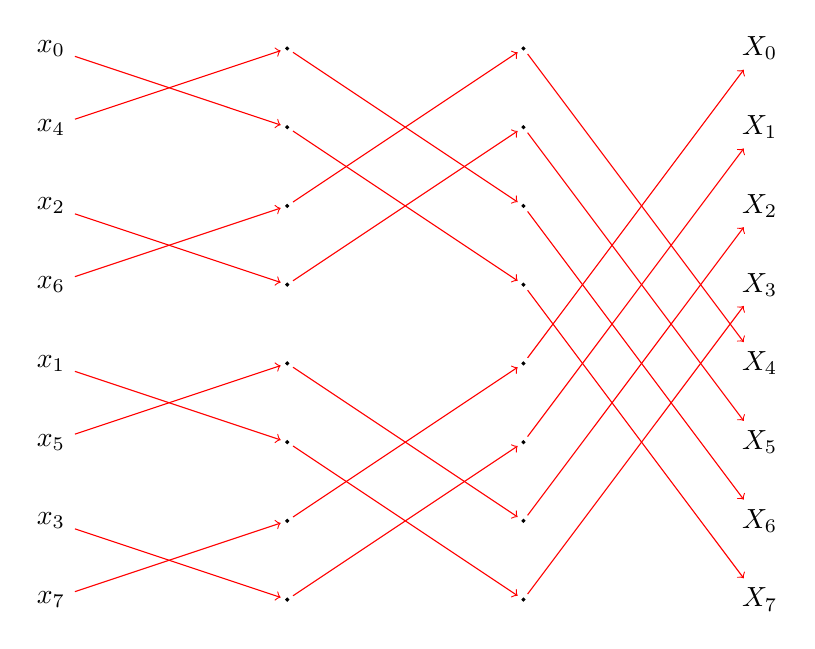
\begin{tikzpicture}[node distance=2cm]

        % nodes
        \node (f0) at (0, 7) {$x_0$};
        \node (f4) at (0, 6) {$x_4$};
        \node (f2) at (0, 5) {$x_2$};
        \node (f6) at (0, 4) {$x_6$};
        \node (f1) at (0, 3) {$x_1$};
        \node (f5) at (0, 2) {$x_5$};
        \node (f3) at (0, 1) {$x_3$};
        \node (f7) at (0, 0) {$x_7$};

        \node [draw,circle,fill=black,inner sep=0pt,outer sep=2pt] (h1) at (3, 7) {};
        \node [draw,circle,fill=black,inner sep=0pt,outer sep=2pt] (h2) at (3, 6) {};
        \node [draw,circle,fill=black,inner sep=0pt,outer sep=2pt] (h3) at (3, 5) {};
        \node [draw,circle,fill=black,inner sep=0pt,outer sep=2pt] (h4) at (3, 4) {};
        \node [draw,circle,fill=black,inner sep=0pt,outer sep=2pt] (h5) at (3, 3) {};
        \node [draw,circle,fill=black,inner sep=0pt,outer sep=2pt] (h6) at (3, 2) {};
        \node [draw,circle,fill=black,inner sep=0pt,outer sep=2pt] (h7) at (3, 1) {};
        \node [draw,circle,fill=black,inner sep=0pt,outer sep=2pt] (h8) at (3, 0) {};

        \node [draw,circle,fill=black,inner sep=0pt,outer sep=2pt] (2h1) at (6, 7) {};
        \node [draw,circle,fill=black,inner sep=0pt,outer sep=2pt] (2h2) at (6, 6) {};
        \node [draw,circle,fill=black,inner sep=0pt,outer sep=2pt] (2h3) at (6, 5) {};
        \node [draw,circle,fill=black,inner sep=0pt,outer sep=2pt] (2h4) at (6, 4) {};
        \node [draw,circle,fill=black,inner sep=0pt,outer sep=2pt] (2h5) at (6, 3) {};
        \node [draw,circle,fill=black,inner sep=0pt,outer sep=2pt] (2h6) at (6, 2) {};
        \node [draw,circle,fill=black,inner sep=0pt,outer sep=2pt] (2h7) at (6, 1) {};
        \node [draw,circle,fill=black,inner sep=0pt,outer sep=2pt] (2h8) at (6, 0) {};

        \node (3h1) at (9, 7) {$X_0$};
        \node (3h2) at (9, 6) {$X_1$};
        \node (3h3) at (9, 5) {$X_2$};
        \node (3h4) at (9, 4) {$X_3$};
        \node (3h5) at (9, 3) {$X_4$};
        \node (3h6) at (9, 2) {$X_5$};
        \node (3h7) at (9, 1) {$X_6$};
        \node (3h8) at (9, 0) {$X_7$};

        % arrows
        % First iteration
        \draw [->,draw=red] (f0) -- (h2);
        \draw [->,draw=red] (f4) -- (h1);
        \draw [->,draw=red] (f2) -- (h4);
        \draw [->,draw=red] (f6) -- (h3);
        \draw [->,draw=red] (f1) -- (h6);
        \draw [->,draw=red] (f5) -- (h5);
        \draw [->,draw=red] (f3) -- (h8);
        \draw [->,draw=red] (f7) -- (h7);

        % Second iteration
        \draw [->,draw=red] (h1) -- (2h3);
        \draw [->,draw=red] (h2) -- (2h4);
        \draw [->,draw=red] (h3) -- (2h1);
        \draw [->,draw=red] (h4) -- (2h2);
        \draw [->,draw=red] (h5) -- (2h7);
        \draw [->,draw=red] (h6) -- (2h8);
        \draw [->,draw=red] (h7) -- (2h5);
        \draw [->,draw=red] (h8) -- (2h6);

        % Third iteration
        \draw [->,draw=red] (2h1) -- (3h5);
        \draw [->,draw=red] (2h2) -- (3h6);
        \draw [->,draw=red] (2h3) -- (3h7);
        \draw [->,draw=red] (2h4) -- (3h8);
        \draw [->,draw=red] (2h5) -- (3h1);
        \draw [->,draw=red] (2h6) -- (3h2);
        \draw [->,draw=red] (2h7) -- (3h3);
        \draw [->,draw=red] (2h8) -- (3h4);
    \end{tikzpicture}
    \caption{Butterfly update for 8 values \cite{fft:derivation}}
    \label{fig:general:butterfly}
\end{figure}

\begin{table}
    \centering
    \caption{Bit reversal conversion table for input size 8}
    \label{tab:rev:table}
    \begin{tabular}{|r|r||r|r|}
        \hline
        \textbf{normal dec} & \textbf{normal bin} & \textbf{reversed bin} & \textbf{reversed dec}\\
        \hline
        \texttt{0} & \texttt{000} & \texttt{000} & \texttt{0} \\
        \texttt{1} & \texttt{001} & \texttt{100} & \texttt{4} \\
        \texttt{2} & \texttt{010} & \texttt{010} & \texttt{2} \\
        \texttt{3} & \texttt{011} & \texttt{110} & \texttt{6} \\
        \texttt{4} & \texttt{100} & \texttt{001} & \texttt{1} \\
        \texttt{5} & \texttt{101} & \texttt{101} & \texttt{5} \\
        \texttt{6} & \texttt{110} & \texttt{011} & \texttt{3} \\
        \texttt{7} & \texttt{111} & \texttt{111} & \texttt{7} \\
        \hline
    \end{tabular}
\end{table}

\begin{figure}
    \centering
    \begin{tikzpicture}[node distance=2cm]

        % nodes
        \node (A) at (0, 0) {$x_b$};
        \node (B) at (0, 1) {$x_a$};
        \node (C) at (3, 0) {$x'_b$};
        \node (D) at (3, 1) {$x'_a$};

        \node [draw,circle,above left=-3mm and 2mm of D,inner sep=0pt] (plus) {$+$};
        \node [draw,circle,below left=-3mm and 2mm of C,inner sep=0pt] (plus) {$-$};
        \node [draw,circle,below right=-2mm and 2mm of A,inner sep=0pt] (plus) {$\times$};

        % arrows
        \draw [->,draw=red] (A) -- (D);
        \draw [->,draw=red] (B) -- (C);

    \end{tikzpicture}
    \caption{Butterfly update \cite{fft:derivation}}
    \label{fig:butterfly:update}
\end{figure}

When we have achieved this, the operation order must be established. For the first iteration, the size of the gap between the operands is one. The next gap size is two and the third is four. It is now possible to construct an iterative algorithm with pseudocode as shown in Algorithm~\ref{alg:fft}. The fist part of the algorithm is the Bit reversal. This has clearly $O(N)$ time complexity assuming the time complexity of bit\_reverse is bounded by the size of an integer. For the butterfly updates, the outer while loop will run for $\log{}N$ iterations and the two inner loops will run a total of $\frac{step}{2} \frac{N}{step} = \frac{N}{2}$ times. It is now clear that the time complexity of this algorithm is $O(N\log{}N)$.


\begin{figure}[H]
    \begin{algorithm}[H]
        \KwData{Complex array $x = x_1, x_2, ..., x_N$ in time domain}
        \KwResult{Complex array $X = X_1, X_2, ..., X_N$ in frequency domain}

        \tcc{Bit reversal}
        \For{$i\gets 0$ \KwTo $N - 1$}{
            $r \gets$ bit\_reverse($i$)\\
            \If{$r > i$}{
                temp $\gets$ $x$[i]\\
                $x$[i] $\gets$ $x$[r]\\
                $x$[r] $\gets$ temp
            }
        }

        \tcc{Butterfly updates}
        $step \gets 2$\\
        \While{$step \leq N$}{
            \For{$k\gets 0$ \KwTo $step/2 - 1$}{
                \For{$p\gets 0$ \KwTo $N/step - 1$}{
                    $curr\gets p * step + k$\\
                    $x$[$curr$] $= x$[$curr$] $+$ $x$[$curr + step/2$]$*\omega^{k}_{step}$\\
                    $x$[$curr + step/2$] $= x$[$curr$] $-$ $x$[$curr + step/2$]$*\omega^{k}_{step}$
                }
            }
            $step \gets 2*step$
        }
        \textbf{return} $x$
        \caption{Iterative FFT}
        \label{alg:fft}
    \end{algorithm}
\end{figure}

\section{Related work}
A study called \emph{FFT benchmark on Android devices: Java versus JNI} \cite{Jr2013} was published in 2013 and investigated how two implementations of FFT performed on different Android devices. The main point of the study was to compare how a pure Java implementation would perform compared to a library written in C called FFTW. This library supports multi-threaded computation and this aspect is also covered in this study. Their benchmark application was run on 35 different devices with different versions to get a wide picture of how the algorithms ran on different phones.

\emph{Evaluating Performance of Android Platform Using Native C for Embedded Systems} \cite{Lee2010} explored how JNI overhead, arithmetic operations, memory access and heap allocation affected an application written in Java and native C. This study was written in 2010 when the Android NDK was relatively new. Since then, many patches has been released, improving performance of code written in native C/C++. In this study, Dalvik VM was the virtual machine that executed the Dalvik bytecode. This study found that the JNI overhead was insignificant and took 0.15 ms to run in their testing environment. Their test results indicated that C was faster than Java in every case. The performance difference was largest in the memory access test and smallest in floating point calculations.

Published in 2016, \emph{Android App Energy Efficiency: The Impact of Language, Runtime, Compiler, and Implementation} \cite{Chen2016} presented a performance comparison between ART and native on Android. The main focus of the report was to find how much more efficient one of them were in terms of energy consumption. Their tests consisted of measuring battery drainage in power as well as execution time of different algorithms. It also compares performance differences between ART and Dalvik. The conclusion states that native performs much better than code running on the Dalvik VM. However, code compiled by ART improves greatly from Dalvik and performs almost the same as code compiled by Android NDK.

\cleardoublepage

\chapter{Method}\label{ch:method}
\textit{To ensure that the experiments were carried out correctly, multiple tools for measurements were evaluated. Different implementations of the FFT were also compared to choose the ones that would typically be used in an Android project.}

\section{Experiment model}

% http://lessthanoptimal.github.io/Java-Matrix-Benchmark/manual/MethodologyRuntimeBenchmark/

In this thesis, different aspects that can affect execution time for an \gls{fft} implementation on Android were tested. To get an overview of how much of an impact they have, the following subjects were investigated:

\begin{enumerate}
    \item Cost of using the \gls{jni}
    \item Compare well known libraries
    \item Vectorization optimization with \gls{neon}, exclusive for native
    \item Using \texttt{float} and \texttt{double} as primary data types
\end{enumerate}

The reason it is relevant to know how significant the \gls{jni} overhead is, is because we want to see for what data size the transition time for going between Java and native is irrelevant compared to the total execution time of the \gls{jni} call. This would also show how much repeated calls to native code would affect the performance of a program. By minimizing the number of calls to the \gls{jni}, a program would potentially get faster.

There are many different implementations of the \gls{fft} publicly available that could be of interest for use in a project. This test demonstrates how different libraries compare. It is helpful to see how viable different implementations are on Android, both for C++ libraries and for Java libraries. It can also be useful to know how small implementations can perform in terms of speed. The sample sizes used for the \gls{fft} can vary depending on the requirements for the implementation.

If the app needs to be efficient, it is common to lower the number of collected samples. This comes at a cost of accuracy. A fast \gls{fft} implementation allows for more data being passed to the \gls{fft}, improving frequency resolution. This is one of the reasons it is important to have a fast \gls{fft}.

Optimizations that are only possible in native code is a good demonstration of how a developer can improve performance even more and to perhaps achieve better execution times than what is possible in Java. Having one single source file is valuable, especially for native libraries. This facilitates the process of adding and editing libraries.

Finally, comparing how performance can change depending on which data types that are used is also interesting when choosing a given implementation. Using the \texttt{float} data type, you use less memory at the cost of precision. A \texttt{double} occupies double the amount of space compared to a \texttt{float}, although it allows higher precision numbers. Caching is one aspect that could be utilized by reducing the space required for the results array.

\subsection{Hardware}
In this thesis, the hardware was delimited to one device to prevent the experiment from being too extensive and allow a more narrow examination of the test performed. The setup used for performing the experiments is described in Table~\ref{tab:hardware}.

\ifrelease
\begin{table}[H]
    \centering
    \label{tab:hardware}
    \caption{Hardware used in the experiments}
    \begin{tabular}{|l|l|}
        \hline
        \textbf{Phone model} & Google Nexus 6P\\
        \hline
        \textbf{CPU model} & Qualcomm MSM8994 Snapdragon 810\\
        \hline
        \textbf{Core frequency} & 4x2.0 GHz and 4x1.55 GHz\\
        \hline
        \textbf{Total RAM} & 3 GB\\
        \hline
        \textbf{Available RAM} & 1.5 GB\\
        \hline
    \end{tabular}
\end{table}
\fi

\subsection{Benchmark Environment}
During the tests, both cellular and Wi-Fi were switched off. There were no applications running in the background while performing the tests during the experiments. Additionally, there were no foreground services running. This was to prevent any external influences from affecting the results. The software versions, compiler versions and compiler flags are presented in Table~\ref{tab:software}. The \texttt{-O3} optimization was used because it resulted in a small performance improvements compared with no optimization. The app was signed and packaged with release as build type. It was then transferred and installed on the device.

\ifrelease
\begin{table}[H]
    \centering
    \caption{Software used in the experiments}
    \begin{tabular}{|l|l|}
        \hline
        \textbf{Android version} & 7.1.1\\
        \hline
        \textbf{Kernel version} & 3.10.73g7196b0d\\
        \hline
        \textbf{Clang/LLVM version} & 3.8.256229\\
        \hline
        \textbf{Java version} & 1.8.0\_76\\
        \hline
        \textbf{Java compiler flags} & \texttt{FLAGS HERE}\\
        \hline
        \textbf{C++ compiler flags} & \texttt{-Wall -std=c++14 -llog -lm -O3}\\
        \hline
    \end{tabular}
    \label{tab:software}
\end{table}
\fi

\subsection{Time measurement}
There are multiple methods of measuring time in Java. It is possible to measure the wall-clock time using the \texttt{System.currentTimeMillis()} method. There are drawbacks of using wall-clock time for measuring time. Because it is possible to manipulate the wall-clock at any time, it could result in too small or too large times depending on seemingly random factors. A more preferable method is to measure elapsed CPU time. This does not depend on a changeable wall-clock but rather it uses hardware to measure time. It is possible to use both \texttt{System.nanoTime()} and \texttt{SystemClock.elapsedRealtimeNanos()} for this purpose and the latter was used for the tests covered in this thesis.

What is being measured is the time to execute the tests assuming we have the desired input data and will get the required output data where we do not convert the data. Different algorithms accepts different data types as input parameters. When using an algorithm, the easiest solution would be to design your application around the algorithm (its input parameters and its return type). When possible to calculate external dependencies such as lookup tables, this is done outside the timer as it is only done once and not for each call to the \gls{fft}.

Some algorithms require a \texttt{Complex[]}, some require a \texttt{double[]} where the first half contains the real numbers and the second half contain the imaginary numbers and some require two double arrays, one for the real numbers and one for imaginary. Because of these different requirements, the timer encapsulates a function shown in Figure~\ref{fig:timer:pos}. The timer would not measure the conversion from the shared input to the input type required by the particular algorithm.

\ifrelease
\begin{figure}
\begin{lstlisting}[
        language={C++},
        basicstyle=\ttfamily\footnotesize,
        keywordstyle=\color{blue}\ttfamily,
        stringstyle=\color{red}\ttfamily,
        commentstyle=\color{green!70!black}\ttfamily,
    ]
    // Prepare formatted input
    double[] z = combineComplex(re, im);

    // Start timer
    long start = SystemClock.elapsedRealtimeNanos();

    // Native call
    double[] nativeResult = fft_princeton_recursive(z);

    // Stop timer
    long stop = SystemClock.elapsedRealtimeNanos() - start;
\end{lstlisting}
\caption{Timer placements for tests}
\label{fig:timer:pos}
\end{figure}
\fi

% \subsection{Memory measurement}
% \hl{TODO:}
% \emph{The profiling tool provided by Android Studio was used to measure the amount of memory that each test required. The method used to measure the memory was to attach the debugger to the app and measure using the profiler. To measure each test separately and equally, the app was launched freshly between tests and the garbage collector was forced before each test. After this, the memory allocation tracker was activated and then followed by starting a test. When the test had been done executing, the tracker was stopped and the results saved. The memory measure tests were executed at a different time than the execution time tests}

\section{Evaluation}
The unit of the resulting data was chosen to be in milliseconds. To be able to have 100 executions run in reasonable time, the maximum size of the input data was limited to $2^{18} = 262144$ for all the tests. We need this many executions of the same test to get statistically significant results. The sampling rate is what determines the highest frequency that could be found in the result. The frequency range perceivable by the human ear ($\sim$ 20-22,000 Hz) is covered by the tests. According to the Nyquist theorem, the sampling rate must be at least twice the upper limit (44,000). Because the \gls{fft} is limited to sample sizes of powers of 2, the next power of 2 for a sampling rate of 44,000 is $2^{16}$. This size was chosen as the upper limit for the library comparisons.

For the SIMD tests, even larger sizes were used. This was to demonstrate how the execution time grew when comparing Java with low level optimizations in C++. Here, sizes up to $2^{18}$ were used because the steps from $2^{16} - 2^{18}$ illustrated this point clearly. It is also with these sizes the garbage collection gets invoked many times due to large allocations.

\subsection{Data representation}
The block sizes chosen in the \gls{jni} and libraries tests are limited to every power of two from $2^4$ to $2^{16}$. For NEON tests, $2^{16} - 2^{18}$ will be used for the tests. One reason this interval was chosen was because it is relevant to have the largest data the largest number of blocks needed for sample rates of 44100 Hz. To get a resolution of at least one Hz for a frequency span of 0-22050 Hz, an \gls{fft} size of $2^{16}$ (next power of two for 44,100) is required. The lowest sample size was chosen to be $2^{4}$ to get a variety of data points to test for to find the increase in execution time for larger data sizes.

Every test result were not presented in Chapter~\ref{ch:results} - Results. In this chapter, only the results that were relevant to discuss about are included. The tests results not found in the results chapter is found in Appendix~\ref{appendix:results}. To visualize a result, tables and line graphs were used. \gls{fft} sizes were split into groups labeled \emph{small} size ($2^{4} - 2^{7}$) \emph{medium} size ($2^{8} - 2^{12}$), \emph{large} size ($2^{13} - 2^{16}$) and \emph{extra large} size ($2^{17} - 2^{18}$). This decision was made to allow the discussion to be divided into groups to see where the difference in performance between the algorithms is significant. An accelerometer samples at low frequencies, commonly at the ones grouped as \emph{small}.

For the normal \gls{fft} tests, the data type \texttt{double} was used and when presenting the results for the optimization tests, \texttt{float} was used. This was to ensure that we could discuss the differences in efficiency for choosing a specific data type.

\subsection{Sources of error}
% https://www2.southeastern.edu/Academics/Faculty/rallain/plab193/labinfo/Error_Analysis/06_Sources_of_Error.html
There are multiple factors that can skew the results when running the tests. Some are controllable and some are not. In these tests, allocation of objects were minimized as much as possible to prevent the overhead of allocating dynamic memory. Because the Java garbage collector is uncontrollable during runtime, this will depend on the sizes of the objects and other aspects dependent on a specific implementation. \gls{jni} allows native code to be run without interruption by the garbage collector by using the \texttt{GetPrimitiveArrayCritical} function call. Additionally, implementation details of the Java libraries were not altered to ensure that the exact library found was used.

% CPU throttling is another factor that can influence the execution times. This is a feature where the CPU changes its clock frequency to reduce heat generated by being in full load for too long. Different phones have different cooling capability and a profiler can provide information if this occurs during a test. 

\subsection{Statistical significance}
Because the execution times differ between runs, it is important to calculate the sample mean and a confidence interval. This way we have an expected value to use in our results as well as being able to say with a chosen certainty that one mean is larger than the other. To get an accurate sample mean, we must have a large sample size. The sample size chosen for the tests in this thesis was 100. The following formula calculates the sample mean \cite[p.263]{olofsson2012probability}:

\begin{equation*}
    \bar{X} = \frac{1}{N} \sum\limits_{k = 1}^{N} X_k
\end{equation*}

Now, the standard deviation is needed to find the dispersion of the data for each test. The standard deviation for a set of random samples $X_1, \dots, X_N$ is calculated using the following formula \cite[p.~302]{olofsson2012probability}:
\begin{equation*}
    s = \sqrt{\frac{1}{N - 1} \sum\limits_{k = 1}^{N}\left(X_k - \bar{X}\right)^2}
\end{equation*}

When comparing results, we need to find a confidence interval for a given test and choose a confidence level. For the data gathered in this study, a 95\% two-sided confidence level was chosen when comparing the data. To find the confidence interval we must first find the standard error of the mean using the following formula \cite[p.~304]{olofsson2012probability}:
\begin{equation*}
    SE_{\bar{X}} = \frac{s}{\sqrt{N}}
\end{equation*}

To find the confidence interval, we must calculate the margin of error by taking the appropriate $z^*$-value for a confidence level and multiplying it with the standard error. For a confidence level of 95\%, we get a margin of error as follows:

\begin{equation*}
    ME_{\bar{X}} = SE_{\bar{X}} \cdot 1.96
\end{equation*}

Our confidence interval will then be:
\begin{equation*}
    \bar{X} \pm ME_{\bar{X}}
\end{equation*}

\section{JNI Tests}
For testing the \gls{jni} overhead, four different tests were constructed. The first test had no parameters, returned void and did no calculations. The purpose of this test was to see how long it would take to call the smallest function possible. The function shown in Figure~\ref{fig:jni:empty} was used to test this.

\begin{figure}[H]
\begin{lstlisting}[
        language={C++},
        basicstyle=\ttfamily\footnotesize,
        keywordstyle=\color{blue}\ttfamily,
        stringstyle=\color{red}\ttfamily,
        commentstyle=\color{green!70!black}\ttfamily,
    ]
                 void jniEmpty(JNIEnv*, jobject) {
                     return;
                 }
\end{lstlisting}
\caption{JNI test function with no parameters and no return value}
\label{fig:jni:empty}
\end{figure}

For the second test, a function was written (see Figure~\ref{fig:jni:params}) that took a jdoubleArray as input and returned the same data type. The reason this test was made was to see if \gls{jni} introduced some extra overhead for passing an argument and having a return value.

\begin{figure}[H]
\begin{lstlisting}[
        language={C++},
        basicstyle=\ttfamily\footnotesize,
        keywordstyle=\color{blue}\ttfamily,
        stringstyle=\color{red}\ttfamily,
        commentstyle=\color{green!70!black}\ttfamily,
    ]
     jdoubleArray jniParams(JNIEnv*, jobject, jdoubleArray arr) {
         return arr;
     }
\end{lstlisting}
\caption{JNI test function with a double array as input parameter and return value}
\label{fig:jni:params}
\end{figure}

In the third test seen in Figure~\ref{fig:jni:conversion}, the \texttt{GetPrimitiveArrayCritical} function was called to be able to access the elements stored in \texttt{arr}. When all the calculations were done, the function would return \texttt{arr}. To overwrite the changes made on \texttt{elements}, a function called \texttt{ReleasePrimitiveArrayCritical} had to be called.

\begin{figure}
\begin{lstlisting}[
        language={C++},
        basicstyle=\ttfamily\footnotesize,
        keywordstyle=\color{blue}\ttfamily,
        stringstyle=\color{red}\ttfamily,
        commentstyle=\color{green!70!black}\ttfamily,
    ]
jdoubleArray jniVectorConversion(JNIEnv* env, jobject, jdoubleArray arr) {
    jdouble* elements = (jdouble*)(*env).GetPrimitiveArrayCritical(arr, 0);
    (*env).ReleasePrimitiveArrayCritical(arr, elements, 0);
    return arr;
}
\end{lstlisting}
\caption{Get and release elements}
\label{fig:jni:conversion}
\end{figure}

The fourth and final test evaluated the performance of passing three arrays through \gls{jni} as well as the cost of getting and releasing the arrays. This test was included because the Columbia algorithm requires the precomputed trigonometric tables. This test is presented in Figure~\ref{fig:jni:columbia}.

\begin{figure}
\begin{lstlisting}[
        language={C++},
        basicstyle=\ttfamily\footnotesize,
        keywordstyle=\color{blue}\ttfamily,
        stringstyle=\color{red}\ttfamily,
        commentstyle=\color{green!70!black}\ttfamily,
    ]
jdoubleArray jniColumbia(JNIEnv* env,
                         jobject obj,
                         jdoubleArray arr,
                         jdoubleArray cos,
                         jdoubleArray sin) {
    jdouble* elements = (jdouble*)(*env).GetPrimitiveArrayCritical(arr, 0);
    jdouble* sin_v    = (jdouble*)(*env).GetPrimitiveArrayCritical(sin, 0);
    jdouble* cos_v    = (jdouble*)(*env).GetPrimitiveArrayCritical(cos, 0);
    (*env).ReleasePrimitiveArrayCritical(arr, elements, 0);
    (*env).ReleasePrimitiveArrayCritical(sin, sin_v, 0);
    (*env).ReleasePrimitiveArrayCritical(cos, cos_v, 0);
    return arr;
}
\end{lstlisting}
\caption{JNI overhead for Columbia FFT}
\label{fig:jni:columbia}
\end{figure}

\section{Fast Fourier Transform Algorithms}
Different implementations of \gls{fft} were used in the libraries test. Three of them were implemented in Java and one in C. The implementations chosen were all contained in one file. The following algorithms were used to compare and find a good estimate on the performance of \gls{fft} implementations with varying complexity:

\begin{itemize}
    \item Princeton Recursive \cite{princeton:recursive}
    \item Princeton Iterative \cite{princeton:iterative}
    \item Columbia Iterative \cite{columbia:iterative}
    \item Kiss (\emph{Keep It Simple, Stupid}) \gls{fft} \cite{kiss:fft}
\end{itemize}

\subsection{Java Libraries}

The Princeton Recursive \gls{fft} is a straightforward implementation of the \gls{fft} with no radical optimizations. It was implemented in Java by Robert Sedgewick and Kevin Wayne \cite{princeton:recursive}. Twiddle factors are trigonometric constants used during the butterfly operations. They are not precomputed in this algorithm, leading to duplicate work when calling it multiple times.

Princeton Iterative, also written by Robert Sedgewick and Kevin Wayne \cite{princeton:iterative}, is an iterative version of the previous \gls{fft} (also written in Java). Iterative bit reversal and butterfly operations are used to produce a faster algorithm.

Columbia Iterative \cite{columbia:iterative} uses pre-computed trigonometric tables that are prepared in the class constructor. Because you commonly call \gls{fft} for the same sizes in your program, it is beneficial to have the trigonometric tables saved and use them in subsequent calls to the \gls{fft}.

\subsection{C++ Libraries}
Conversion to C++ was done manually for Princeton Iterative, Princeton Recursive and Columbia Iterative. Some changes were necessary to follow the C++ syntax. The Complex class used in Java was replaced by \texttt{std::complex} in all converted programs. Java dynamic arrays were replaced by \texttt{std::vector} for when they were created. This only occurred in the Princeton Recursive algorithm. In Princeton Iterative and Columbia Iterative, a Java array reference was sent to the function and there were no arrays created in the functions. In C++, a pointer and a variable containing the array size was used instead.

Kiss \gls{fft} is a small library that consists of one source file. It is available under the BSD license. To use it, you first call the \texttt{kiss\_fft\_alloc} function which allocates memory for the twiddle factors as well as calculates them. This function returns a struct object that is used as a config. The \gls{fft} is executed when the \texttt{kiss\_fft} function is called. The first parameter for this function is the config returned by the init function, followed by a pointer to the time domain input and a pointer to where the frequency output will be placed.

\section{NEON Optimization}
% => http://edp.org/work/Construction.pdf <== OPTIMIZATION
% https://aaltodoc.aalto.fi/bitstream/handle/123456789/23201/master_Sugawara_Koki_2016.pdf?sequence=1

Two libraries were chosen to test how vectorization of the loops can improve performance. Both libraries were written in Intel SSE intrinsics and were converted to ARM NEON intrinsics. \texttt{float} was used so that the vector registers could hold 4 elements. It is possible to have the register hold two double precision variables although this would increase the number of instructions needed to calculate the \gls{fft}. For memory locality, this is also inefficient.

The first \gls{fft} algorithm was a recursive implementation written by Anthony Blake~\cite{neon:recursive}. This algorithm has an initializer function that allocates space for the twiddle factors and calculates them. They are placed in a two dimensional array that utilizes memory locality to waste less memory bandwidth \cite{neon:recursive:details}. The converted program is listed in Appendix~\ref{lst:recursive:neon}. The second algorithm was an iterative implementation. This library is a straightforward implementation of \gls{fft} with SSE \cite{code:manyears} and was written for a sound source localization system \cite{manyears:site}. The code that was converted from SSE to NEON is presented in Appendix~\ref{lst:iterative:neon}.

\cleardoublepage

\chapter{Results}\label{ch:results}
\textit{Results from the JNI tests, FFT libraries, NEON optimizations and Garbage Collection are presented here.}

%%==================================================================
%% JNI-Tests
%%==================================================================
\section{JNI}
The results from the tests that measure the JNI overhead can be found in Table~\ref{tab:jni:common}. These tests are presented with block sizes defined in Chapter~\ref{ch:method} - Method. Execution time and confidence intervals are given in microseconds and are rounded to four decimal points. The number before the $\pm$ sign is the sample mean and the number after $\pm$ is a two sided confidence interval with a confidence level of $95\%$. Each test was executed 100 times to ensure that we get reliable sample means. As well as having tests that run in reasonable time.

The test labeled \textbf{No params} is the test where a native void function with no parameters that returns immediately was called. \textbf{Vector} takes a \texttt{jdoubleArray} and returns a \texttt{jdoubleArray} immediately. \textbf{Convert} takes a \texttt{jdoubleArray}, converts it to a native array using \texttt{GetPrimitiveArrayCritical()}, converts it back to a \texttt{jdoubleArray} using \texttt{ReleasePrimitiveArrayCritical()} and returns a \texttt{jdoubleArray}. \textbf{Columbia} takes three \texttt{jdoubleArray}s, converts them and returns them the same way as \textbf{Convert} does.

No surprising data regarding the first two tests were found. Neither the \textbf{No params} nor \textbf{Vector} tests had a clear increase in execution time for an increase in block size. \textbf{Vector} did have a higher mean for block size \textbf{65536}. On the other hand, we can see that the 95\% confidence interval is very large ($\pm 3.1960$ \textmu s). This is likely due to its high standard deviation of 16.3058 found in Appendix~\ref{appendix:results} Table~\ref{tab:appendix:raw:jni:vector}. Likewise, there is a spike in execution time mean for block size \textbf{1024} in the \textbf{Convert} test.

\ifrelease
\begin{table}[H]
    \centering
    \caption{Results from the JNI tests, Time (\textmu s)}
    \label{tab:jni:common}
    \rowcolors{1}{}{lightgray}
\begin{tabular}{lrrrr}\toprule
\textbf{Block size}  & \textbf{No params} & \textbf{Vector} & \textbf{Convert} & \textbf{Columbia}\\\midrule
\textbf{16}  & 1.7922 $\pm$ 0.1392 & 1.9333 $\pm$ 0.1223 & 2.6052 $\pm$ 0.1004 & 4.1058 $\pm$ 0.3042\\
\textbf{32}  & 1.6983 $\pm$ 0.0220 & 2.8130 $\pm$ 1.7924 & 2.6006 $\pm$ 0.0370 & 3.9109 $\pm$ 0.0535\\
\textbf{64}  & 1.6755 $\pm$ 0.0149 & 1.6344 $\pm$ 0.1809 & 2.6630 $\pm$ 0.0425 & 3.9296 $\pm$ 0.0566\\
\textbf{128}  & 1.9604 $\pm$ 0.4978 & 1.2349 $\pm$ 0.1262 & 1.9375 $\pm$ 0.0843 & 3.0823 $\pm$ 0.0892\\
\textbf{256}  & 1.7292 $\pm$ 0.0694 & 1.3276 $\pm$ 0.2589 & 1.8141 $\pm$ 0.0276 & 3.0958 $\pm$ 0.0441\\
\textbf{512}  & 1.6916 $\pm$ 0.0110 & 1.2567 $\pm$ 0.1227 & 2.2818 $\pm$ 0.7011 & 3.1656 $\pm$ 0.0457\\
\textbf{1024}  & 2.0228 $\pm$ 0.5684 & 1.3167 $\pm$ 0.1341 & 6.3756 $\pm$ 8.4676 & 3.2896 $\pm$ 0.1396\\
\textbf{2048}  & 1.7218 $\pm$ 0.0288 & 1.5416 $\pm$ 0.1405 & 1.9099 $\pm$ 0.0898 & 3.4844 $\pm$ 0.1113\\
\textbf{4096}  & 1.1411 $\pm$ 0.0404 & 1.4010 $\pm$ 0.0788 & 2.0062 $\pm$ 0.1562 & 3.8562 $\pm$ 0.3197\\
\textbf{8192}  & 1.1105 $\pm$ 0.0078 & 1.4818 $\pm$ 0.0759 & 2.3671 $\pm$ 0.1897 & 3.8474 $\pm$ 0.4784\\
\textbf{16384}  & 1.1183 $\pm$ 0.0280 & 1.7308 $\pm$ 0.1043 & 2.5833 $\pm$ 0.1737 & 4.9724 $\pm$ 0.8955\\
\textbf{32768}  & 1.1162 $\pm$ 0.0084 & 2.2099 $\pm$ 0.1880 & 3.2062 $\pm$ 0.2029 & 5.3719 $\pm$ 0.2875\\
\textbf{65536}  & 1.7463 $\pm$ 1.2217 & 4.7474 $\pm$ 3.1960 & 4.3198 $\pm$ 0.2926 & 6.8136 $\pm$ 0.2499\\
\textbf{131072}  & 1.1027 $\pm$ 0.0141 & 2.6375 $\pm$ 0.1531 & 5.7004 $\pm$ 0.2681 & 9.6912 $\pm$ 1.4337\\
\textbf{262144} & 1.1006 $\pm$ 0.0118 & 3.3172 $\pm$ 0.1164 & 7.4630 $\pm$ 0.2309 & 10.2781 $\pm$ 0.2278\\
\bottomrule
\end{tabular}

\end{table}
\fi


%%==================================================================
%% FFT-Tests
%%==================================================================
\section{FFT Libraries}
The results from the FFT Libraries are presented in line graphs, both language specific and graphs with both Java and C++. They are given to illustrate the differences between languages and also provide differences for specific languages clearly. The time unit for these tests are presented in milliseconds. This was because the FFT ran in ranges below one millisecond and above one second among different algorithms and different block sizes. The means were calculated from the results of 100 test runs.  In each C++ line graph, the fastest Java test was added to make it easier to get a reference and compare the languages.

%=========%
%= SMALL =%
%=========%
\subsection{Small block sizes}
Results from the small blocks tests shows a clear difference between the different algorithms. In Figure~\ref{fig:all:line:small}, Princeton Recursive in Java perform the worst. Princeton Recursive in C++ and Princeton Iterative in Java perform better than Princeton Recursive Java although worse than the rest of the algorithms. The rest of the algorithms perform similarly and does not seem to grow with larger block sizes.

\ifrelease
\begin{figure}
    \centering
    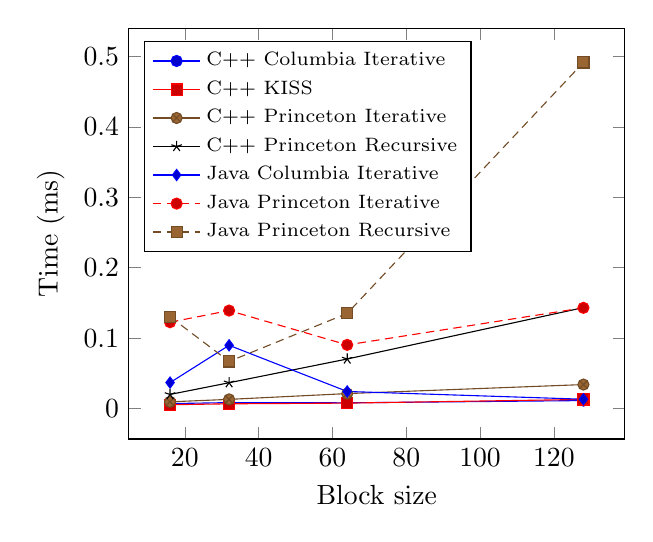
\begin{tikzpicture}
\begin{axis}[xlabel={Block size},ylabel={Time (ms)},width=0.65\linewidth,legend pos=north west,scaled y ticks = false,legend cell align=left,legend style={font=\scriptsize}]
\addplot coordinates {
(16, 0.0072)
(32, 0.0086)
(64, 0.0083)
(128, 0.0115)
};
\addplot coordinates {
(16, 0.0056)
(32, 0.0069)
(64, 0.0079)
(128, 0.0131)
};
\addplot coordinates {
(16, 0.0097)
(32, 0.0132)
(64, 0.0214)
(128, 0.0342)
};
\addplot coordinates {
(16, 0.0202)
(32, 0.0368)
(64, 0.0705)
(128, 0.1434)
};
\addplot coordinates {
(16, 0.0370)
(32, 0.0899)
(64, 0.0244)
(128, 0.0134)
};
\addplot coordinates {
(16, 0.1227)
(32, 0.1392)
(64, 0.0905)
(128, 0.1431)
};
\addplot coordinates {
(16, 0.1304)
(32, 0.0670)
(64, 0.1352)
(128, 0.4913)
};
\legend{C++ Columbia Iterative,C++ KISS,C++ Princeton Iterative,C++ Princeton Recursive,Java Columbia Iterative,Java Princeton Iterative,Java Princeton Recursive}
\end{axis}
\end{tikzpicture}

    \caption{Line graph for all algorithms, \emph{small} block sizes}
    \label{fig:all:line:small}
\end{figure}
\fi

As we can see in Figure~\ref{fig:java:line:small}, the standard deviation of Princeton Recursive and Princeton Iterative are very large. This means that the samples were sparse and as a result of this, not a reliable mean. We can see in Table~\ref{tab:java:small} that the confidence interval is generally larger for Princeton Iterative and Princeton Recursive compared to Columbia Iterative.

\ifrelease
\begin{figure}
    \centering
    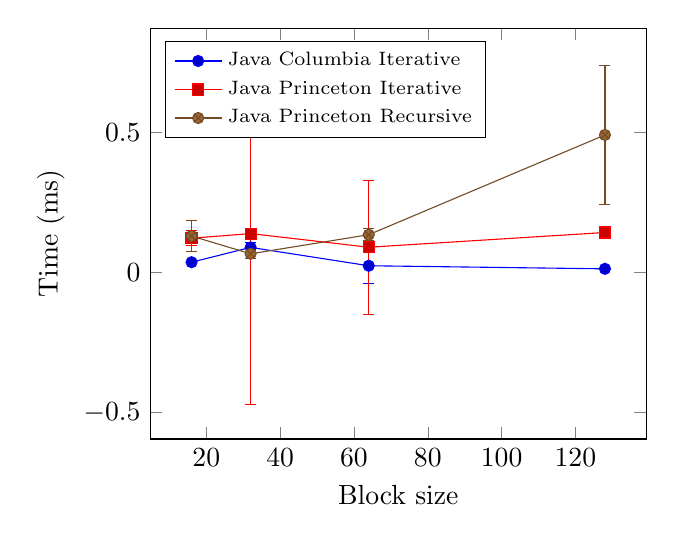
\begin{tikzpicture}
\begin{axis}[xlabel={Block size},ylabel={Time (ms)},width=0.65\linewidth,legend pos=north west,scaled y ticks = false,legend cell align=left,legend style={font=\scriptsize}]
\addplot+[error bars/.cd, y dir=both,y explicit] coordinates {
(16, 0.0370) +- (0.0055, 0.0055)
(32, 0.0899) +- (0.0169, 0.0169)
(64, 0.0244) +- (0.0637, 0.0637)
(128, 0.0134) +- (0.0005, 0.0005)
};
\addplot+[error bars/.cd, y dir=both,y explicit] coordinates {
(16, 0.1227) +- (0.0268, 0.0268)
(32, 0.1392) +- (0.6110, 0.6110)
(64, 0.0905) +- (0.2393, 0.2393)
(128, 0.1431) +- (0.0097, 0.0097)
};
\addplot+[error bars/.cd, y dir=both,y explicit] coordinates {
(16, 0.1304) +- (0.0546, 0.0546)
(32, 0.0670) +- (0.0177, 0.0177)
(64, 0.1352) +- (0.0215, 0.0215)
(128, 0.4913) +- (0.2475, 0.2475)
};
\legend{Java Columbia Iterative , Java Princeton Iterative , Java Princeton Recursive}
\end{axis}
\end{tikzpicture}

    \caption{Java line graph for \emph{small} block sizes with standard deviation error bars}
    \label{fig:java:line:small}
\end{figure}
\fi

\ifrelease
\begin{table}
    \centering
    \caption{Java results table for \emph{small} block sizes, Time (ms)}
    \label{tab:java:small}
    \rowcolors{1}{}{lightgray}
\begin{tabular}{lccc}\toprule
\textbf{Block size}  & \textbf{Columbia Iterative} & \textbf{Princeton Iterative} & \textbf{Princeton Recursive}\\\midrule
\textbf{16}  & 0.0370 $\pm$ 0.0010 & 0.1227 $\pm$ 0.0053 & 0.1304 $\pm$ 0.0108\\
\textbf{32}  & 0.0899 $\pm$ 0.0033 & 0.1392 $\pm$ 0.1198 & 0.0670 $\pm$ 0.0035\\
\textbf{64}  & 0.0244 $\pm$ 0.0125 & 0.0905 $\pm$ 0.0468 & 0.1352 $\pm$ 0.0043\\
\textbf{128} & 0.0134 $\pm$ 0.0002 & 0.1431 $\pm$ 0.0020 & 0.4913 $\pm$ 0.0486\\
\bottomrule
\end{tabular}

\end{table}
\fi

As for the C++ tests, the results were less scattered and had a more apparent increase in time with increasing block sizes. We can also see that the slowest algorithm, Princeton Recursive, has the largest standard deviation. It is clear by looking at Table~\ref{tab:cpp:small} that KISS performs the best, followed by Columbia Iterative, Princeton Iterative and then Princeton Recursive. If we look at the Java implementation, it has a general decrease in execution time for larger block sizes although it is faster than Princeton Iterative and Recursive.

\ifrelease
\begin{figure}
    \centering
    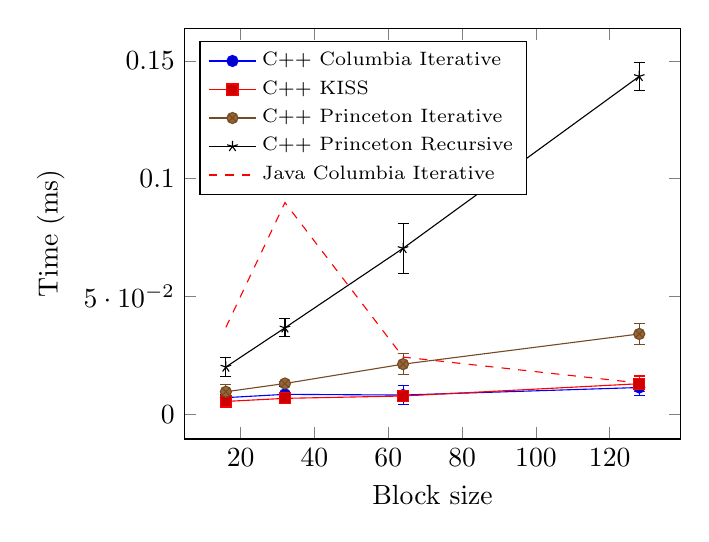
\begin{tikzpicture}
\begin{axis}[xlabel={Block size},ylabel={Time (ms)},width=0.65\linewidth,legend pos=north west,scaled y ticks = false,legend cell align=left,legend style={font=\scriptsize}]
\addplot+[error bars/.cd, y dir=both,y explicit] coordinates {
(16, 0.0072) +- (0.0012, 0.0012)
(32, 0.0086) +- (0.0034, 0.0034)
(64, 0.0083) +- (0.0041, 0.0041)
(128, 0.0115) +- (0.0033, 0.0033)
};
\addplot+[error bars/.cd, y dir=both,y explicit] coordinates {
(16, 0.0056) +- (0.0013, 0.0013)
(32, 0.0069) +- (0.0005, 0.0005)
(64, 0.0079) +- (0.0009, 0.0009)
(128, 0.0131) +- (0.0033, 0.0033)
};
\addplot+[error bars/.cd, y dir=both,y explicit] coordinates {
(16, 0.0097) +- (0.0032, 0.0032)
(32, 0.0132) +- (0.0009, 0.0009)
(64, 0.0214) +- (0.0044, 0.0044)
(128, 0.0342) +- (0.0045, 0.0045)
};
\addplot+[error bars/.cd, y dir=both,y explicit] coordinates {
(16, 0.0202) +- (0.0039, 0.0039)
(32, 0.0368) +- (0.0038, 0.0038)
(64, 0.0705) +- (0.0105, 0.0105)
(128, 0.1434) +- (0.0059, 0.0059)
};
\addplot+[style=dashed,color=red,mark=none] coordinates {
(16, 0.0370) +- (0.0055, 0.0055)
(32, 0.0899) +- (0.0169, 0.0169)
(64, 0.0244) +- (0.0637, 0.0637)
(128, 0.0134) +- (0.0005, 0.0005)
};
\legend{C++ Columbia Iterative , C++ KISS , C++ Princeton Iterative , C++ Princeton Recursive, Java Columbia Iterative}
\end{axis}
\end{tikzpicture}

    \caption{C++ line graph for \emph{small} block sizes with standard deviation error bars}
    \label{fig:cpp:line:small}
\end{figure}
\fi

\ifrelease
\begin{table}
    \centering
    \caption{C++ results table for \emph{small} block sizes, Time (ms)}
    \label{tab:cpp:small}
    \resizebox{\columnwidth}{!}{%
        \rowcolors{1}{}{lightgray}
\begin{tabular}{lrrrr}\toprule
\textbf{Block size}  & \textbf{Columbia Iterative} & \textbf{KISS} & \textbf{Princeton Iterative} & \textbf{Princeton Recursive}\\\midrule
\textbf{16}  & 0.007 $\pm$ 0.0002 & 0.005 $\pm$ 0.0002 & 0.009 $\pm$ 0.0006 & 0.020 $\pm$ 0.0008\\
\textbf{32}  & 0.008 $\pm$ 0.0006 & 0.006 $\pm$ 0.0002 & 0.013 $\pm$ 0.0002 & 0.036 $\pm$ 0.0008\\
\textbf{64}  & 0.008 $\pm$ 0.0008 & 0.007 $\pm$ 0.0002 & 0.021 $\pm$ 0.0008 & 0.070 $\pm$ 0.0022\\
\textbf{128} & 0.011 $\pm$ 0.0006 & 0.013 $\pm$ 0.0006 & 0.034 $\pm$ 0.0008 & 0.143 $\pm$ 0.0012\\
\bottomrule
\end{tabular}

    }
\end{table}
\fi


%==========%
%= MEDIUM =%
%==========%
\subsection{Medium block sizes}
The medium block sizes (Figure~\ref{fig:all:line:medium}) continues the trend where Java Princeton Recursive performs the worst followed by Java Princeton Iterative and C++ Princeton Recursive. As for the small block sizes, Java Columbia Iterative, C++ Princeton Iterative, C++ Columbia Iterative and KISS have the smallest execution time and perform similarly.

\ifrelease
\begin{figure}
    \centering
    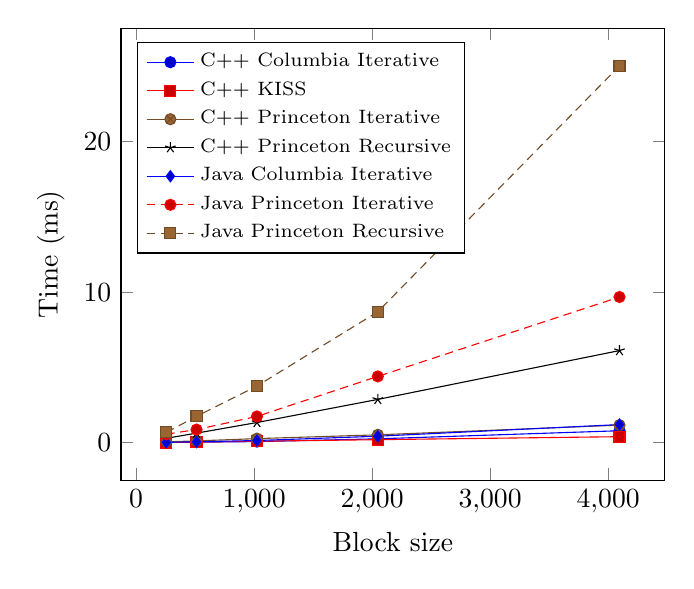
\begin{tikzpicture}
\begin{axis}[xlabel={Block size},ylabel={Time (ms)},width=0.70\linewidth,legend pos=north west,scaled y ticks = false,legend cell align=left,legend style={font=\scriptsize}]
\addplot coordinates {
(256, 0.0200)
(512, 0.0366)
(1024, 0.0773)
(2048, 0.2604)
(4096, 0.7974)
};
\addplot coordinates {
(256, 0.0182)
(512, 0.0461)
(1024, 0.0992)
(2048, 0.2047)
(4096, 0.4022)
};
\addplot coordinates {
(256, 0.0627)
(512, 0.1225)
(1024, 0.2744)
(2048, 0.5257)
(4096, 1.1701)
};
\addplot coordinates {
(256, 0.2978)
(512, 0.6379)
(1024, 1.3437)
(2048, 2.8773)
(4096, 6.1206)
};
\addplot coordinates {
(256, 0.0293)
(512, 0.0615)
(1024, 0.1484)
(2048, 0.4338)
(4096, 1.2071)
};
\addplot coordinates {
(256, 0.5698)
(512, 0.8758)
(1024, 1.7488)
(2048, 4.4055)
(4096, 9.6792)
};
\addplot coordinates {
(256, 0.6929)
(512, 1.7515)
(1024, 3.7688)
(2048, 8.6983)
(4096, 25.0276)
};
\legend{C++ Columbia Iterative,C++ KISS,C++ Princeton Iterative,C++ Princeton Recursive,Java Columbia Iterative,Java Princeton Iterative,Java Princeton Recursive}
\end{axis}
\end{tikzpicture}

    \caption{Line graph for all algorithms, \emph{medium} block sizes}
    \label{fig:all:line:medium}
\end{figure}
\fi

The results found in Figure~\ref{fig:java:line:medium} are somewhat different than for the small block sizes. We can still see that Java Princeton Recursive diverges from the other algorithms. What is interesting is that it is now clearer which of Princeton Iterative and Columbia Iterative is the fastest. Columbia Iterative is clearly faster than Princeton Iterative as shown by the confidence intervals given in Table~\ref{tab:java:medium}. The standard deviations for the samples in the Princeton Recursive and Princeton Iterative are still relatively large compared to Columbia Iterative.

\ifrelease
\begin{figure}
    \centering
    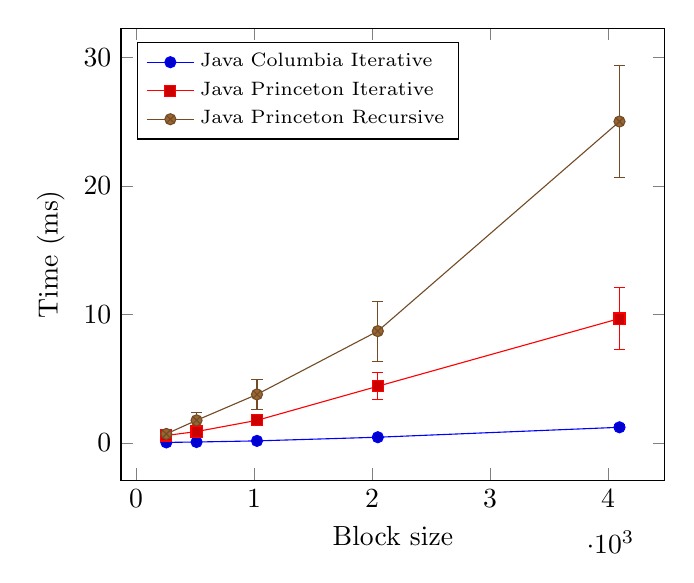
\begin{tikzpicture}
\begin{axis}[xlabel={Block size},ylabel={Time (ms)},width=0.70\linewidth,legend pos=north west,scaled x ticks={base 10:-3},legend cell align=left,legend style={font=\scriptsize}]
\addplot+[error bars/.cd, y dir=both,y explicit] coordinates {
(256, 0.0293) +- (0.0042, 0.0042)
(512, 0.0615) +- (0.0047, 0.0047)
(1024, 0.1484) +- (0.0308, 0.0308)
(2048, 0.4338) +- (0.0806, 0.0806)
(4096, 1.2071) +- (0.1807, 0.1807)
};
\addplot+[error bars/.cd, y dir=both,y explicit] coordinates {
(256, 0.5698) +- (0.4834, 0.4834)
(512, 0.8758) +- (0.3145, 0.3145)
(1024, 1.7488) +- (0.3452, 0.3452)
(2048, 4.4055) +- (1.0527, 1.0527)
(4096, 9.6792) +- (2.3947, 2.3947)
};
\addplot+[error bars/.cd, y dir=both,y explicit] coordinates {
(256, 0.6929) +- (0.1662, 0.1662)
(512, 1.7515) +- (0.6352, 0.6352)
(1024, 3.7688) +- (1.1879, 1.1879)
(2048, 8.6983) +- (2.3341, 2.3341)
(4096, 25.0276) +- (4.3322, 4.3322)
};
\legend{Java Columbia Iterative , Java Princeton Iterative , Java Princeton Recursive}
\end{axis}
\end{tikzpicture}

    \caption{Java line graph for \emph{medium} block sizes with standard deviation error bars}
    \label{fig:java:line:medium}
\end{figure}
\fi

\ifrelease
\begin{table}
    \centering
    \caption{Java results table for \emph{medium} block sizes, Time (ms)}
    \label{tab:java:medium}
    \rowcolors{1}{}{lightgray}
\begin{tabular}{lccc}\toprule
\textbf{Block size}  & \textbf{Columbia Iterative} & \textbf{Princeton Iterative} & \textbf{Princeton Recursive}\\\midrule
\textbf{256}  & 0.0293 $\pm$ 0.0008 & 0.5698 $\pm$ 0.0947 & 0.6929 $\pm$ 0.0325\\
\textbf{512}  & 0.0615 $\pm$ 0.0010 & 0.8758 $\pm$ 0.0615 & 1.7515 $\pm$ 0.1245\\
\textbf{1024}  & 0.1484 $\pm$ 0.0061 & 1.7488 $\pm$ 0.0676 & 3.7688 $\pm$ 0.2328\\
\textbf{2048}  & 0.4338 $\pm$ 0.0159 & 4.4055 $\pm$ 0.2064 & 8.6983 $\pm$ 0.4575\\
\textbf{4096} & 1.2071 $\pm$ 0.0355 & 9.6792 $\pm$ 0.4694 & 25.0276 $\pm$ 0.8491\\
\bottomrule
\end{tabular}

\end{table}
\fi

For the C++ algorithms, it is now apparent which order the algorithms rank regarding performance found in Figure~\ref{fig:cpp:line:medium}. Princeton Recursive perform the worst while the rest has similar execution times. It is now clear that KISS performs best, followed by Columbia Iterative and then Princeton Iterative. The Java Columbia Iterative implementation proves to be faster than Princeton for block sizes smaller than 4096.

In Table~\ref{tab:cpp:medium} we can see that the confidence intervals are relatively small, meaning these results have higher precision than for the same test with smaller block sizes. We can also see that there is no overlap between any confidence intervals thereby giving us a strong indication that the order in performance given in the previous paragraph is true.

\ifrelease
\begin{figure}
    \centering
    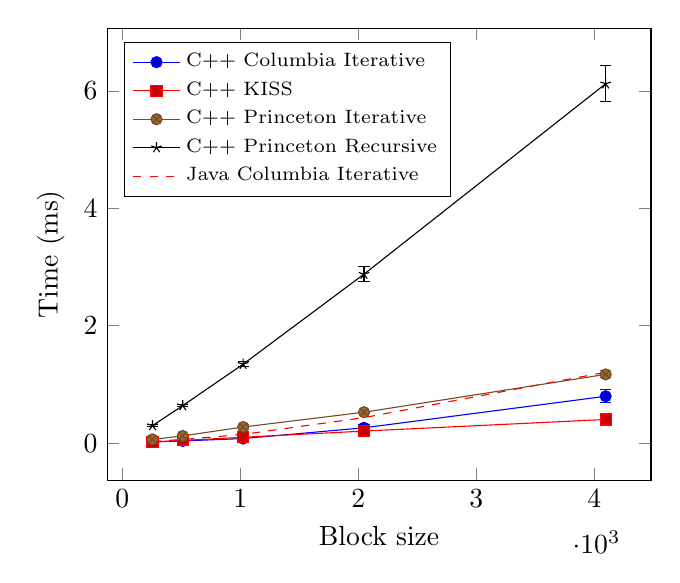
\begin{tikzpicture}
\begin{axis}[xlabel={Block size},ylabel={Time (ms)},width=0.70\linewidth,legend pos=north west,scaled x ticks={base 10:-3},legend cell align=left,legend style={font=\scriptsize}]
\addplot+[error bars/.cd, y dir=both,y explicit] coordinates {
(256, 0.0200) +- (0.0043, 0.0043)
(512, 0.0366) +- (0.0033, 0.0033)
(1024, 0.0773) +- (0.0097, 0.0097)
(2048, 0.2604) +- (0.0634, 0.0634)
(4096, 0.7974) +- (0.1097, 0.1097)
};
\addplot+[error bars/.cd, y dir=both,y explicit] coordinates {
(256, 0.0182) +- (0.0037, 0.0037)
(512, 0.0461) +- (0.0110, 0.0110)
(1024, 0.0992) +- (0.0883, 0.0883)
(2048, 0.2047) +- (0.0765, 0.0765)
(4096, 0.4022) +- (0.0625, 0.0625)
};
\addplot+[error bars/.cd, y dir=both,y explicit] coordinates {
(256, 0.0627) +- (0.0040, 0.0040)
(512, 0.1225) +- (0.0032, 0.0032)
(1024, 0.2744) +- (0.0495, 0.0495)
(2048, 0.5257) +- (0.0185, 0.0185)
(4096, 1.1701) +- (0.0602, 0.0602)
};
\addplot+[error bars/.cd, y dir=both,y explicit] coordinates {
(256, 0.2978) +- (0.0127, 0.0127)
(512, 0.6379) +- (0.0181, 0.0181)
(1024, 1.3437) +- (0.0445, 0.0445)
(2048, 2.8773) +- (0.1288, 0.1288)
(4096, 6.1206) +- (0.3046, 0.3046)
};
\addplot+[style=dashed,color=red,mark=none] coordinates {
(256, 0.0293) +- (0.0042, 0.0042)
(512, 0.0615) +- (0.0047, 0.0047)
(1024, 0.1484) +- (0.0308, 0.0308)
(2048, 0.4338) +- (0.0806, 0.0806)
(4096, 1.2071) +- (0.1807, 0.1807)
};
\legend{C++ Columbia Iterative , C++ KISS , C++ Princeton Iterative , C++ Princeton Recursive, Java Columbia Iterative}
\end{axis}
\end{tikzpicture}

    \caption{C++ line graph for \emph{medium} block sizes with standard deviation error bars}
    \label{fig:cpp:line:medium}
\end{figure}
\fi

\ifrelease
\begin{table}[H]
    \centering
    \caption{C++ results table for \emph{medium} block sizes, Time (ms)}
    \label{tab:cpp:medium}
    \resizebox{\columnwidth}{!}{%
        \rowcolors{1}{}{lightgray}
\begin{tabular}{lrrrr}\toprule
\textbf{Block size}  & \textbf{Columbia Iterative} & \textbf{KISS} & \textbf{Princeton Iterative} & \textbf{Princeton Recursive}\\\midrule
\textbf{256}  & 0.02 $\pm$ 0.0008 & 0.01 $\pm$ 0.0008 & 0.06 $\pm$ 0.0008 & 0.29 $\pm$ 0.0025\\
\textbf{512}  & 0.03 $\pm$ 0.0006 & 0.04 $\pm$ 0.0022 & 0.12 $\pm$ 0.0006 & 0.63 $\pm$ 0.0035\\
\textbf{1024}  & 0.07 $\pm$ 0.0020 & 0.09 $\pm$ 0.0172 & 0.27 $\pm$ 0.0098 & 1.34 $\pm$ 0.0086\\
\textbf{2048}  & 0.26 $\pm$ 0.0123 & 0.20 $\pm$ 0.0149 & 0.52 $\pm$ 0.0035 & 2.87 $\pm$ 0.0253\\
\textbf{4096} & 0.79 $\pm$ 0.0216 & 0.40 $\pm$ 0.0123 & 1.17 $\pm$ 0.0118 & 6.12 $\pm$ 0.0598\\
\bottomrule
\end{tabular}

    }
\end{table}
\fi

%=========%
%= LARGE =%
%=========%
\subsection{Large block sizes}
Figure~\ref{fig:all:line:large} shows the growth in execution time for increasing block sizes of type \emph{large}. It continues the trend set by the tests with a block size of \emph{medium}. It is easy to see which algorithms that perform worse than the others. As previous tests shows, Java Princeton Recursive, Java Princeton Iterative and C++ Princeton Recursive are still the slowest.

\ifrelease
\begin{figure}
    \centering
    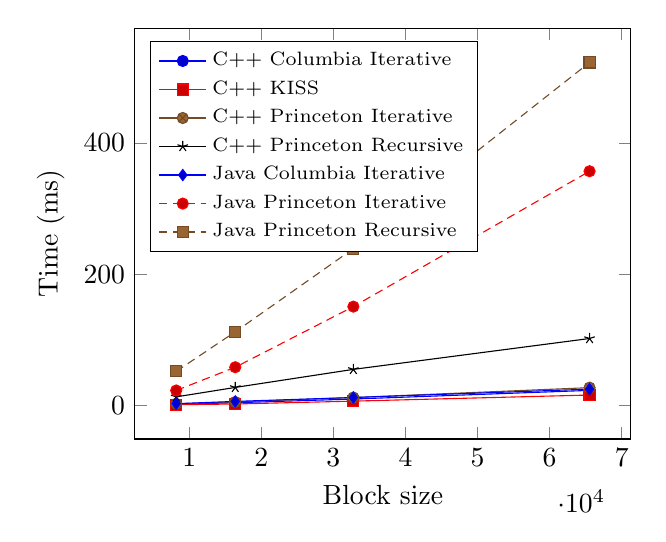
\begin{tikzpicture}
\begin{axis}[xlabel={Block size},ylabel={Time (ms)},width=0.65\linewidth,legend pos=north west,scaled y ticks = false,legend cell align=left,legend style={font=\scriptsize}]
\addplot coordinates {
(8192, 1.9326)
(16384, 4.2789)
(32768, 9.9388)
(65536, 23.1031)
};
\addplot coordinates {
(8192, 1.2470)
(16384, 2.3713)
(32768, 6.7420)
(65536, 16.0281)
};
\addplot coordinates {
(8192, 2.5845)
(16384, 5.4518)
(32768, 12.2266)
(65536, 27.2805)
};
\addplot coordinates {
(8192, 13.2345)
(16384, 27.6080)
(32768, 55.1227)
(65536, 102.1585)
};
\addplot coordinates {
(8192, 2.8726)
(16384, 6.3214)
(32768, 12.2634)
(65536, 24.9874)
};
\addplot coordinates {
(8192, 22.9609)
(16384, 58.3825)
(32768, 150.7299)
(65536, 356.9871)
};
\addplot coordinates {
(8192, 52.0853)
(16384, 112.3024)
(32768, 239.0777)
(65536, 522.7409)
};
\legend{C++ Columbia Iterative,C++ KISS,C++ Princeton Iterative,C++ Princeton Recursive,Java Columbia Iterative,Java Princeton Iterative,Java Princeton Recursive}
\end{axis}
\end{tikzpicture}

    \caption{Line graph for all algorithms, \emph{large} block sizes}
    \label{fig:all:line:large}
\end{figure}
\fi

The results for the Java tests with \emph{large} block sizes are presented in Figure~\ref{fig:java:line:large}. The results from \emph{large} verifies the order in which the algorithms performs. The order in performance for Java is still Columbia Iterative, Princeton Iterative and Princeton Recursive (where Columbia Iterative is the fastest).

\ifrelease
\begin{figure}
    \centering
    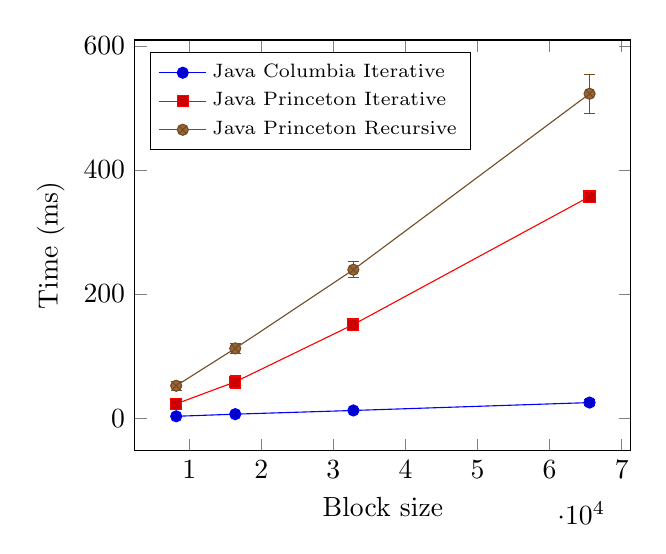
\begin{tikzpicture}
\begin{axis}[xlabel={Block size},ylabel={Time (ms)},width=0.65\linewidth,legend pos=north west,legend cell align=left,legend style={font=\scriptsize}]
\addplot+[error bars/.cd, y dir=both,y explicit] coordinates {
(8192, 2.8726) +- (0.3247, 0.3247)
(16384, 6.3214) +- (1.0542, 1.0542)
(32768, 12.2634) +- (2.9076, 2.9076)
(65536, 24.9874) +- (4.6266, 4.6266)
};
\addplot+[error bars/.cd, y dir=both,y explicit] coordinates {
(8192, 22.9609) +- (5.6248, 5.6248)
(16384, 58.3825) +- (9.9410, 9.9410)
(32768, 150.7299) +- (5.5432, 5.5432)
(65536, 356.9871) +- (8.0942, 8.0942)
};
\addplot+[error bars/.cd, y dir=both,y explicit] coordinates {
(8192, 52.0853) +- (7.1292, 7.1292)
(16384, 112.3024) +- (8.1890, 8.1890)
(32768, 239.0777) +- (12.8962, 12.8962)
(65536, 522.7409) +- (31.4586, 31.4586)
};
\legend{Java Columbia Iterative , Java Princeton Iterative , Java Princeton Recursive}
\end{axis}
\end{tikzpicture}

    \caption{Java line graph for \emph{large} block sizes with standard deviation error bars}
    \label{fig:java:line:large}
\end{figure}
\fi
\ifrelease
\begin{table}
    \centering
    \caption{Java results table for \emph{large} block sizes, Time (ms)}
    \label{tab:java:large}
    \rowcolors{1}{}{lightgray}
\begin{tabular}{lccc}\toprule
\textbf{Block size}  & \textbf{Columbia Iterative} & \textbf{Princeton Iterative} & \textbf{Princeton Recursive}\\\midrule
\textbf{8192}  & 2.8726 $\pm$ 0.0637 & 22.9609 $\pm$ 1.1025 & 52.0853 $\pm$ 1.3973\\
\textbf{16384}  & 6.3214 $\pm$ 0.2066 & 58.3825 $\pm$ 1.9484 & 112.3024 $\pm$ 1.6050\\
\textbf{32768}  & 12.2634 $\pm$ 0.5700 & 150.7299 $\pm$ 1.0864 & 239.0777 $\pm$ 2.5276\\
\textbf{65536} & 24.9874 $\pm$ 0.9069 & 356.9871 $\pm$ 1.5864 & 522.7409 $\pm$ 6.1660\\
\bottomrule
\end{tabular}

\end{table}
\fi

Results for tests with \emph{large} block sizes in C++ produced some interesting results. In Figure~\ref{fig:cpp:line:large} Princeton Recursive has a much larger standard deviation than the other algorithms. It is also the slowest (see Table~\ref{tab:cpp:large}). We can also see in the same table that all algorithms are faster in C++ than their equivalent in Java and that there are no overlapping confidence intervals for a given algorithm or block size. Another thing to note is that the Columbia Iterative algorithm performs almost the same between Java and C++. This is not the case for Princeton Iterative or Recursive.

\ifrelease
\begin{figure}
    \centering
    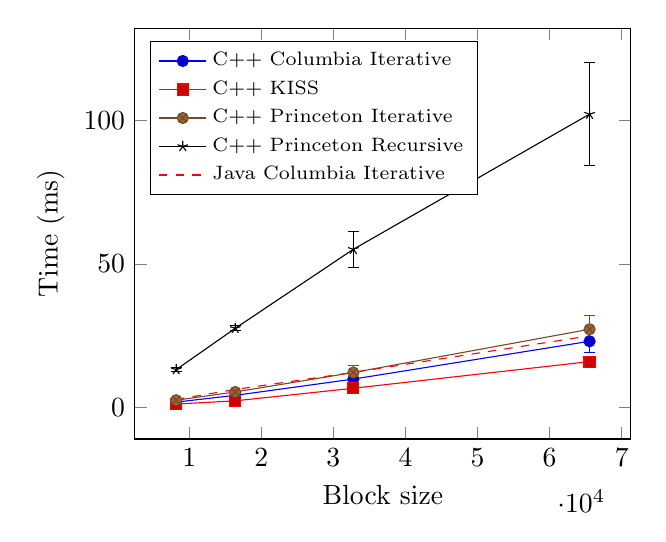
\begin{tikzpicture}
\begin{axis}[xlabel={Block size},ylabel={Time (ms)},width=0.65\linewidth,legend pos=north west,scaled y ticks = false,legend cell align=left,legend style={font=\scriptsize}]
\addplot+[error bars/.cd, y dir=both,y explicit] coordinates {
(8192, 1.9326) +- (0.2654, 0.2654)
(16384, 4.2789) +- (0.6399, 0.6399)
(32768, 9.9388) +- (1.6341, 1.6341)
(65536, 23.1031) +- (3.9019, 3.9019)
};
\addplot+[error bars/.cd, y dir=both,y explicit] coordinates {
(8192, 1.2470) +- (0.2301, 0.2301)
(16384, 2.3713) +- (0.4915, 0.4915)
(32768, 6.7420) +- (1.2931, 1.2931)
(65536, 16.0281) +- (1.8073, 1.8073)
};
\addplot+[error bars/.cd, y dir=both,y explicit] coordinates {
(8192, 2.5845) +- (0.2085, 0.2085)
(16384, 5.4518) +- (0.5858, 0.5858)
(32768, 12.2266) +- (2.4651, 2.4651)
(65536, 27.2805) +- (4.8616, 4.8616)
};
\addplot+[error bars/.cd, y dir=both,y explicit] coordinates {
(8192, 13.2345) +- (0.7311, 0.7311)
(16384, 27.6080) +- (0.9098, 0.9098)
(32768, 55.1227) +- (6.2636, 6.2636)
(65536, 102.1585) +- (17.9911, 17.9911)
};
\addplot+[style=dashed,color=red,mark=none] coordinates {
(8192, 2.8726) +- (0.3247, 0.3247)
(16384, 6.3214) +- (1.0542, 1.0542)
(32768, 12.2634) +- (2.9076, 2.9076)
(65536, 24.9874) +- (4.6266, 4.6266)
};
\legend{C++ Columbia Iterative , C++ KISS , C++ Princeton Iterative , C++ Princeton Recursive, Java Columbia Iterative}
\end{axis}
\end{tikzpicture}

    \caption{C++ line graph for \emph{large} block sizes with standard deviation error bars}
    \label{fig:cpp:line:large}
\end{figure}
\fi
\ifrelease
\begin{table}
    \centering
    \caption{C++ results table for \emph{large} block sizes, Time (ms)}
    \label{tab:cpp:large}
    \resizebox{\columnwidth}{!}{%
        \rowcolors{1}{}{lightgray}
\begin{tabular}{lrrrr}\toprule
\textbf{Block size}  & \textbf{Columbia Iterative} & \textbf{KISS} & \textbf{Princeton Iterative} & \textbf{Princeton Recursive}\\\midrule
\textbf{8192}  & 1.9326 $\pm$ 0.0519 & 1.2470 $\pm$ 0.0451 & 2.5845 $\pm$ 0.0410 & 13.2345 $\pm$ 0.1433\\
\textbf{16384}  & 4.2789 $\pm$ 0.1254 & 2.3713 $\pm$ 0.0962 & 5.4518 $\pm$ 0.1149 & 27.6080 $\pm$ 0.1784\\
\textbf{32768}  & 9.9388 $\pm$ 0.3203 & 6.7420 $\pm$ 0.2534 & 12.2266 $\pm$ 0.4831 & 55.1227 $\pm$ 1.2277\\
\textbf{65536} & 23.1031 $\pm$ 0.7648 & 16.0281 $\pm$ 0.3542 & 27.2805 $\pm$ 0.9530 & 102.1585 $\pm$ 3.5262\\
\bottomrule
\end{tabular}

    }
\end{table}
\fi

%%==================================================================
%% NEON-Tests
%%==================================================================
\section{Optimizations}
The NEON optimizations proved to be very efficient for \emph{extra large} block sizes. These results can be found in Table~\ref{tab:neon:extra}. Comparing these figures with the results, for the same block sizes in Java (Table~\ref{tab:java:float:extra}), we can see that the results from the NEON tests are more than double the speed of the fastest Java implementation. Note that the data type for all of the optimization tests (as well as the C++ and Java tests) were \texttt{float}. Because we get faster execution time by lining up more elements, the \texttt{float} data type was used in the NEON optimizations. When comparing this with non-NEON tests, \texttt{float}s were used in Java and C++ to make the results more comparable.

\ifrelease
\begin{table}[H]
    \centering
    \caption{NEON \texttt{float} results table for \emph{extra large} block sizes, Time (ms)}
    \label{tab:neon:extra}
    \rowcolors{1}{}{lightgray}
\begin{tabular}{lrr}\toprule
\textbf{Block size}  & \textbf{Iterative} & \textbf{Recursive}\\\midrule
\textbf{8192}  & 1.00 $\pm$ 0.01 & 1.61 $\pm$ 0.02\\
\textbf{16384}  & 2.15 $\pm$ 0.05 & 3.56 $\pm$ 0.08\\
\textbf{32768}  & 4.78 $\pm$ 0.15 & 7.60 $\pm$ 0.18\\
\textbf{65536}  & 9.88 $\pm$ 0.24 & 16.11 $\pm$ 0.37\\
\textbf{131072}  & 27.81 $\pm$ 0.71 & 34.16 $\pm$ 0.47\\
\textbf{262144} & 63.18 $\pm$ 1.26 & 74.07 $\pm$ 1.06\\
\bottomrule
\end{tabular}

\end{table}
\fi


Table~\ref{tab:java:float:extra} also show that for very large block sizes, Princeton Iterative and Princeton Recursive are very inefficient compared to Columbia Iterative. This also holds true for the C++ implementation. For these block sizes, however, the differences in execution time is smaller than for Java (as seen in Table~\ref{tab:cpp:float:extra}).

When comparing the NEON results from Table~\ref{tab:neon:extra} with the results from the C++ tests found in Table~\ref{tab:cpp:float:extra}, it is clear that vectorization as an optimization is beneficial. NEON intrinsics resulted in almost twice as fast execution time in comparison with the normal C++ tests. It was also much faster than Java, especially compared to Java Princeton Iterative/Recursive.

In Figure~\ref{fig:neon:line:extra} both the Iterative NEON and the Recursive NEON seems to have the same growth in execution time with increasing block size. Of these two algorithms, Iterative is the fastest. If we compare the results found for Java in Table~\ref{tab:java:float:extra} with the C++ results in Table~\ref{tab:cpp:float:extra} there is a big difference between the Princeton algorithms. The execution times are much larger in Java than in C++. The Java Columbia Iterative is faster than C++ Princeton Iterative for block sizes of 65536.

As we can see in Table~\ref{tab:java:double:extra}, the results show that when using \texttt{double}s, the performance will be worse for Columbia Iterative and Princeton Recursive. We can see that the \texttt{float} tests were always running faster than the corresponding \texttt{double} test.  

\ifrelease
\begin{table}
    \centering
    \caption{Java \texttt{float} results table for \emph{extra large} block sizes, Time (ms)}
    \label{tab:java:float:extra}
    \rowcolors{1}{}{lightgray}
\begin{tabular}{lrrr}\toprule
\textbf{Block size}  & \textbf{Columbia Iterative} & \textbf{Princeton Iterative} & \textbf{Princeton Recursive}\\\midrule
\textbf{8192}  & 2.17 $\pm$ 0.06 & 21.17 $\pm$ 0.66 & 50.07 $\pm$ 1.48\\
\textbf{16384}  & 3.99 $\pm$ 0.09 & 46.81 $\pm$ 1.03 & 103.96 $\pm$ 3.09\\
\textbf{32768}  & 8.98 $\pm$ 0.25 & 113.19 $\pm$ 3.95 & 219.02 $\pm$ 5.56\\
\textbf{65536}  & 20.28 $\pm$ 0.47 & 261.99 $\pm$ 9.19 & 485.10 $\pm$ 13.37\\
\textbf{131072}  & 47.29 $\pm$ 1.30 & 622.43 $\pm$ 24.90 & 1039.49 $\pm$ 26.97\\
\textbf{262144} & 156.71 $\pm$ 1.19 & 1728.46 $\pm$ 53.80 & 2297.80 $\pm$ 58.29\\
\bottomrule
\end{tabular}

\end{table}
\fi

\ifrelease
\begin{table}
    \centering
    \caption{Java \texttt{double} results table for \emph{extra large} block sizes, Time (ms)}
    \label{tab:java:double:extra}
    \resizebox{\columnwidth}{!}{%
        \rowcolors{1}{}{lightgray}
\begin{tabular}{lrrr}\toprule
\textbf{Block size}  & \textbf{Columbia Iterative} & \textbf{Princeton Iterative} & \textbf{Princeton Recursive}\\\midrule
\textbf{8192}  & 2.87 $\pm$ 0.06 & 22.96 $\pm$ 1.10 & 52.08 $\pm$ 1.39\\
\textbf{16384}  & 6.32 $\pm$ 0.20 & 58.38 $\pm$ 1.94 & 112.30 $\pm$ 1.60\\
\textbf{32768}  & 12.26 $\pm$ 0.57 & 150.72 $\pm$ 1.08 & 239.07 $\pm$ 2.52\\
\textbf{65536}  & 24.98 $\pm$ 0.90 & 356.98 $\pm$ 1.58 & 522.74 $\pm$ 6.16\\
\textbf{131072}  & 85.94 $\pm$ 1.60 & 815.86 $\pm$ 3.43 & 1144.88 $\pm$ 17.87\\
\textbf{262144} & 274.51 $\pm$ 5.11 & 2108.07 $\pm$ 27.53 & 2638.05 $\pm$ 40.54\\
\bottomrule
\end{tabular}

    }
\end{table}
\fi

\ifrelease
\begin{table}
    \centering
    \caption{C++ \texttt{float} results table for \emph{extra large} block sizes, Time (ms)}
    \label{tab:cpp:float:extra}
    \resizebox{\columnwidth}{!}{%
        \rowcolors{1}{}{lightgray}
\begin{tabular}{lccc}\toprule
\textbf{Block size}  & \textbf{Columbia Iterative} & \textbf{Princeton Iterative} & \textbf{Princeton Recursive}\\\midrule
\textbf{8192}  & 1.8030 $\pm$ 0.1929 & 2.0605 $\pm$ 0.0110 & 10.7496 $\pm$ 0.0512\\
\textbf{16384}  & 2.9629 $\pm$ 0.1311 & 4.5027 $\pm$ 0.0341 & 22.8640 $\pm$ 0.1748\\
\textbf{32768}  & 8.2847 $\pm$ 0.2364 & 9.6797 $\pm$ 0.1288 & 48.0022 $\pm$ 0.2458\\
\textbf{65536}  & 18.8158 $\pm$ 0.5494 & 20.3049 $\pm$ 0.3467 & 96.9572 $\pm$ 0.2658\\
\textbf{131072}  & 43.7807 $\pm$ 1.2632 & 44.5770 $\pm$ 0.9577 & 192.4607 $\pm$ 5.9702\\
\textbf{262144} & 134.8093 $\pm$ 2.0115 & 129.5150 $\pm$ 1.8201 & 398.9698 $\pm$ 12.9207\\
\bottomrule
\end{tabular}

    }
\end{table}
\fi

\ifrelease
\begin{table}
    \centering
    \caption{C++ \texttt{double} results table for \emph{extra large} block sizes, Time (ms)}
    \label{tab:cpp:double:extra}
    \resizebox{\columnwidth}{!}{%
        \rowcolors{1}{}{lightgray}
\begin{tabular}{lrrrr}\toprule
\textbf{Block size}  & \textbf{Columbia Iterative} & \textbf{KISS} & \textbf{Princeton Iterative} & \textbf{Princeton Recursive}\\\midrule
\textbf{8192}  & 1.93 $\pm$ 0.05 & 1.24 $\pm$ 0.04 & 2.58 $\pm$ 0.04 & 13.23 $\pm$ 0.14\\
\textbf{16384}  & 4.27 $\pm$ 0.12 & 2.37 $\pm$ 0.09 & 5.45 $\pm$ 0.11 & 27.60 $\pm$ 0.17\\
\textbf{32768}  & 9.93 $\pm$ 0.32 & 6.74 $\pm$ 0.25 & 12.22 $\pm$ 0.48 & 55.12 $\pm$ 1.22\\
\textbf{65536}  & 23.10 $\pm$ 0.76 & 16.02 $\pm$ 0.35 & 27.28 $\pm$ 0.95 & 102.15 $\pm$ 3.52\\
\textbf{131072}  & 75.49 $\pm$ 1.64 & 41.76 $\pm$ 0.59 & 78.95 $\pm$ 1.93 & 231.26 $\pm$ 6.73\\
\textbf{262144} & 243.84 $\pm$ 1.00 & 102.11 $\pm$ 1.08 & 250.48 $\pm$ 5.27 & 494.70 $\pm$ 13.66\\
\bottomrule
\end{tabular}

    }
\end{table}
\fi

\ifrelease
\begin{figure}
    \centering
    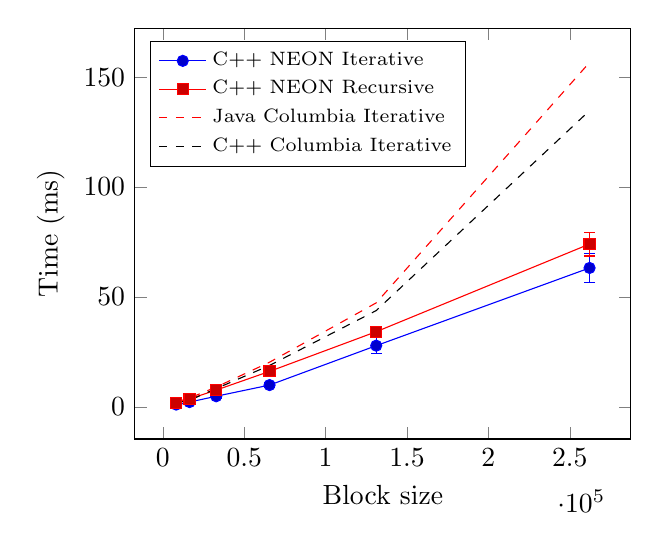
\begin{tikzpicture}
\begin{axis}[xlabel={Block size},ylabel={Time (ms)},width=0.65\linewidth,legend pos=north west,scaled y ticks = false,legend cell align=left,legend style={font=\scriptsize}]
\addplot+[error bars/.cd, y dir=both,y explicit] coordinates {
(8192, 1.0051) +- (0.0657, 0.0657)
(16384, 2.1559) +- (0.2562, 0.2562)
(32768, 4.7898) +- (0.7872, 0.7872)
(65536, 9.8807) +- (1.2509, 1.2509)
(131072, 27.8158) +- (3.6457, 3.6457)
(262144, 63.1858) +- (6.4595, 6.4595)
};
\addplot+[error bars/.cd, y dir=both,y explicit] coordinates {
(8192, 1.6133) +- (0.1416, 0.1416)
(16384, 3.5690) +- (0.4367, 0.4367)
(32768, 7.6009) +- (0.9583, 0.9583)
(65536, 16.1129) +- (1.8936, 1.8936)
(131072, 34.1650) +- (2.4085, 2.4085)
(262144, 74.0746) +- (5.4424, 5.4424)
};
\addplot+[style=dashed,color=red,mark=none] coordinates {
(8192, 2.1766) +- (0.3256, 0.3256)
(16384, 3.9995) +- (0.4596, 0.4596)
(32768, 8.9846) +- (1.3089, 1.3089)
(65536, 20.2833) +- (2.4423, 2.4423)
(131072, 47.2950) +- (6.6700, 6.6700)
(262144, 156.7135) +- (6.0892, 6.0892)
};
\addplot+[style=dashed,color=black,mark=none] coordinates {
(8192, 1.8030) +- (0.9841, 0.9841)
(16384, 2.9629) +- (0.6687, 0.6687)
(32768, 8.2847) +- (1.2061, 1.2061)
(65536, 18.8158) +- (2.8032, 2.8032)
(131072, 43.7807) +- (6.4454, 6.4454)
(262144, 134.8093) +- (10.2633, 10.2633)
};
\legend{C++ NEON Iterative , C++ NEON Recursive, Java Columbia Iterative, C++ Columbia Iterative}
\end{axis}
\end{tikzpicture}

    \caption{NEON results table for \emph{extra large} block sizes, Time (ms)}
    \label{fig:neon:line:extra}
\end{figure}
\fi

%%==================================================================
%% Memory-Tests
%%==================================================================
% \section{Memory tests}
%
% \begin{table}
%     \centering
%     \caption{Total runtime allocation, one call, for block size 262144, Memory (bytes)}
%     \label{tab:result:memory}
%     \rowcolors{1}{}{lightgray}
%     \begin{tabular}{lr}\toprule
%         \textbf{Block size} & \textbf{Memory} \\\midrule
%         \textbf{Java Columbia Iterative} & \\
%         \textbf{Java Princeton Iterative} & \\
%         \textbf{Java Princeton Recursive} & \\
%         \textbf{Java Float Columbia Iterative} & \\
%         \textbf{Java Float Princeton Iterative} & \\
%         \textbf{Java Float Princeton Recursive} & 1,571,016\\
%         \textbf{C++ Columbia Iterative} & \\
%         \textbf{C++ Princeton Iterative} & \\
%         \textbf{C++ Princeton Recursive} & \\
%         \textbf{C++ Float Columbia Iterative} & 0\\
%         \textbf{C++ Float Princeton Iterative} & 0\\
%         \textbf{C++ Float Princeton Recursive} & 0\\
%         \textbf{KISS} & 0\\
%         \textbf{NEON Iterative} & 0 \\
%         \textbf{NEON Recursive} & 0 \\
%     \bottomrule
%     \end{tabular}
% \end{table}

%%==================================================================
%% GC trigger
%%==================================================================
\section{Garbage Collection}
\label{ch:gc}
Table~\ref{tab:result:gc:trigger} shows how many garbage collections that were triggered during the tests. Each row includes all block sizes and 100 iterations for one algorithm. This figure lists the number of partial Concurrent Mark Sweeps, the sum of its garbage collection pauses, the number of sticky Concurrent Mark Sweeps and the sum of its garbage collection pauses.

\ifrelease
\begin{table}[H]
    \centering
    \caption{Pauses due to garbage collection}
    \label{tab:result:gc:trigger}
    \resizebox{\columnwidth}{!}{%
        \rowcolors{1}{}{lightgray}
        \begin{tabular}{|l|rr|rr|}\toprule
            \textbf{Algorithm} & \textbf{\# partial} & \textbf{tot. time (ms)} & \textbf{\# sticky} & \textbf{tot. time (ms)}\\\midrule
            \textbf{Java Columbia Iterative}        & 0 & 0 & 0 & 0\\
            % \textbf{Java Princeton Iterative}       & 336 & 2,016.48 & 349 & 2,046.88\\
            \textbf{Java Princeton Iterative}       & 477 & 2,825.52 & 406 & 2,959.24\\
            % \textbf{Java Princeton Recursive}       & 360 & 645.88 & 85 & 486.97\\
            \textbf{Java Princeton Recursive}       & 240 & 602.10 & 397 & 887.39\\
            \textbf{Java Float Columbia Iterative}  & 0 & 0 & 0 & 0\\
            % \textbf{Java Float Princeton Iterative} & 400 & 2,791.10 & 325 & 2,627.63\\
            \textbf{Java Float Princeton Iterative} & 269 & 1,541.97 & 334 & 2,316.53\\
            % \textbf{Java Float Princeton Recursive} & 356 & 635.12 & 466 & 1,035.78\\
            \textbf{Java Float Princeton Recursive} & 167 & 313.05 & 27 & 71.39\\
            \textbf{C++ Columbia Iterative}         & 0 & 0 & 0 & 0\\
            \textbf{C++ Princeton Iterative}        & 0 & 0 & 0 & 0\\
            \textbf{C++ Princeton Recursive}        & 0 & 0 & 0 & 0\\
            \textbf{C++ Float Columbia Iterative}   & 0 & 0 & 0 & 0\\
            \textbf{C++ Float Princeton Iterative}  & 0 & 0 & 0 & 0\\
            \textbf{C++ Float Princeton Recursive}  & 0 & 0 & 0 & 0\\
            \textbf{KISS}                           & 0 & 0 & 0 & 0\\
            \textbf{NEON Iterative}                 & 0 & 0 & 0 & 0\\
            \textbf{NEON Recursive}                 & 0 & 0 & 0 & 0\\
        \bottomrule
        \end{tabular}
    }
\end{table}
\fi

Table~\ref{tab:result:gc:trigger:2} shows the block size at which each algorithm first triggered the garbage collector. This data is relevant because we can see if there is a possibility to reduce the risk of triggering the garbage collector for different block sizes. This can also be significant in the discussion about how \texttt{float}s and \texttt{double}s perform. When the garbage collector is running, we can see that the pauses can be between 0.468-23.760 ms as seen in the raw data\footnote{https://github.com/anddani/thesis/tree/master/gc\_results}.

\ifrelease
\begin{table}[H]
    \centering
    \caption{Block size where each algorithm started to trigger garbage collection}
    \label{tab:result:gc:trigger:2}
    \rowcolors{1}{}{lightgray}
    \begin{tabular}{lr}\toprule
        \textbf{Algorithm} & \textbf{Block Size}\\\midrule
        \textbf{Princeton Iterative} & 8192\\
        \textbf{Princeton Recursive} & 4096\\
        \textbf{Float Princeton Iterative} & 16384\\
        \textbf{Float Princeton Recursive} & 8192\\
        \bottomrule
    \end{tabular}
\end{table}
\fi

\cleardoublepage

\chapter{Discussion}\label{ch:discussion}
\textit{The discussion chapter covers how the JNI affects performance, how efficient smaller FFT libraries are, why the optimization gave the results found in Chapter~\ref{ch:results} - Results and the efficiency difference between floats and doubles.}

\section{JNI Overhead}
The test results from the JNI tests showed that the overhead is small relative to the computation of the FFT algorithm. As long as it is being run once per calculation, it will not affect the performance significantly. If the JNI is called in a loop when it might not be necessary, the overhead add up and becomes a larger part of the total execution time. Another thing to note is that the execution time stay within about 10 \textmu s. They are also not growing with larger input.

The confidence intervals overlap for many of the values, meaning we cannot say whether or not one input yields a faster execution time than the other. Some larger block sizes has lower execution time than smaller block sizes and some grow for larger input. Because of this, it is reasonable to assume that nothing is done to the arrays when they are passed to the JNI, only pointers are copied. The \texttt{GetPrimitiveArrayCritical()} and \texttt{ReleasePrimitiveArrayCritical()} seem to introduce overhead when used on larger arrays. % <= CITE THIS ... as described in

Regarding the spike in mean in the JNI tests, this can be a cause of one large execution time, skewing the results. This is actually the case for the \textbf{Convert} tests with block size 1024 as seen in Figure~\ref{fig:raw:jni:convert:1024} found in Appendix B. A reason for this could be that the garbage collector began executing during the timing of the test.

% The second tests compared the execution times for measuring the benefits of using a critical zone in native code. In Figure~\ref{}

\section{Simplicity and Efficiency} % FFT-libraries

% Which is slowest and why (discussion)??
The slowest algorithm was the Java Princeton Recursive. The reason for this is because it does many method calls. Additionally, each call creates new \texttt{Complex} arrays when splitting up the array in odd and even indices. Lastly, when combining the arrays, new \texttt{Complex} objects are created each time an operation is done between two complex numbers. The \texttt{Complex} class creates immutable objects.

The C++ version of the Princeton Recursive algorithm is faster than the Java version. One big difference is that the \texttt{std::complex} type used in C++ does not create new instances each time is is being operated with. Instead, they are placed on the stack. This lowers the number of calls requesting more memory from the heap. Depending on the situation for the program, there is a risk that the program must ask the system for more memory, slowing down the allocation process.

Additionally, this will increase the work for the garbage collector, increasing the risk of it being triggered during the timing. To prevent the number of allocations you are doing inside a repeated process is to reuse allocated memory. This is done by pre-allocating the necessary arrays or other data structures and overwrite the results for each call. Avoiding calls to new in a method that is called multiple times can increase time and memory efficiency.

% Which is fastest and why (discussion)??
Of the algorithms tested in the FFT library tests, KISS FFT was the fastest. It is more optimized than the \enquote{basic} implementations found in the Columbia and Princeton algorithms. In C++, Princeton Iterative and Columbia Iterative were the fastest and in Java, Columbia Iterative was the fastest. The reason for it being faster in C++ is, as for Java Princeton Recursive, because it uses the \texttt{Complex} class to represent complex numbers. Because Java Columbia Iterative used double arrays to represent real and imaginary numbers, no new objects needed to be created.

% Which tests triggered the GC??
The results from Chapter~\ref{ch:gc} show that the Java Princeton algorithms caused the GC to run. This behaviour was as expected because they called new during their execution. Java Columbia did not cause any garbage collection as well as any of the C++ algorithms.

% Precision (smaller intervals) for larger block sizes C++. Because larger execution times result in more consistent execution times??
% \hilight{Precision (smaller intervals) for larger block sizes C++.}\\
% \hilight{Because larger execution times result in more consistent execution times??}

One thing that is clear is that the Columbia Iterative algorithm is the best one to choose from of the Java versions. It performs better than both Princeton Iterative and Princeton Recursive. It also allows simple modifications such as changing between using \texttt{float}s or  \texttt{double}s to represent the data.

The reason Princeton Iterative and Princeton Recursive is slower in Java than in C++ is because they operate with \texttt{Complex} elements. Each time two \texttt{Complex} numbers are added, multiplied or subtracted, a new \texttt{Complex} object is created. This slows down the process and increases memory consumption, increasing work for the garbage collector.

% Although you can have two equally long implementations, one could be faster than the other.  It is important to do small tests with different sized data.
As we have seen in the tests, choosing an iterative implementation is preferable and choosing the correctly implemented iterative implementation is also important. It is possible to compare implementations by setting up small tests. This is a small time investment that can impact the performance of a program significantly. It is also possible to scan through the implementation, looking for places where it allocates memory and edit it so that it uses an already allocated array. This reduces the number of calls for more memory which lessens the chance of a garbage collect.

% We can see in the tests that the best option is to choose KISS fft as it is the fastest of the options. BUT WHY??
% \hilight{We can see in the tests that the best option is to choose KISS fft as it is the fastest of the options.}


% For smaller Block sizes, the Java version is as fast as the C++ one. It is easier to implement and more flexible to edit. No need for complicated JNI integration.
Comparing the Java and C++ implementations of the Columbia Iterative FFT, for \emph{small}-\emph{large} block sizes, the Java version is almost exactly as fast as the C++ version. For the block sizes added in the \emph{extra large} group, the C++ version perform better. If you were to choose between the C++ and the Java variant of Columbia, it is arguably better to choose the Java version. Avoiding having to implement a JNI bridge between Java and native is more preferable than the almost non-existent boost in performance.

Another argument why it is sensible to choose the Java version is that is has enough performance for processing to allow graphical rendering in 60 \gls{fps}. Let's say we have an application that visualizes sound with a sampling frequency of 44100 Hz and updates the screen at 60 frames per second. It has 16.66 ms to do all the processing needed between the screen updates. If we want to have double precision numbers and use Java it is possible to do an FFT with a size of \textbf{32768}.

This size is more than needed and would require a delay of $32768/44100\approx 743 $ ms and the fastest Java algorithm for double point precision ran in $12$ ms for this block size. As we can see, in relation, the time it takes to execute an FFT is only a small fraction of the time it takes to gather the same number of samples. This is important because it allows larger FFT sizes from the sampled audio, increasing the frequency resolution in the results, while still being sufficiently fast.

% \hilight{some size + FFT overhead < 16.66 ms}
% \hilight{Motivate the frequency resolution received here as well}

For smaller block sizes (\emph{medium} and \emph{large}), common when sampling low frequencies such as speech and acceleration data, it is relevant to have a fast transform for these sizes. Comparing C++ and Java we see that Java is not that much slower, at best, than C++. This gives an incentive to use Java, allowing more consistent code and does not add the complexity of JNI.

% It is with very large block sizes the difference is clear. 
When the block sizes are large, a bigger difference is found between the algorithms. One reason for this is the impact the garbage collection has when triggered during the timing of an algorithm. The pauses can be, depending on the work done in the garbage collect, around \hilight{MIN-MAX} ms.
% \hilight{It is with very large block sizes the difference is clear.}\\
% \hilight{Point to the differences for the largest block sizes for java v c++}

% Discuss differences in performance large java times, small java times WHY?
% \hilight{Discuss differences in performance large java times, small java times WHY?}

KISS FFT was the fastest of all the native implementations. This was because of the optimizations done to improve its performance. Using multiple radix implementations of the FFT, it is possible to get more performance at the cost of higher code complexity. It shows the potential in doing small optimizations that does not rely on multi-core or other architecture dependent optimization techniques.

\section{Vectorization as Optimization}

As the results show, vectorization was an improvement in regards to efficiency. This was as expected because it is possible to process more elements for each instruction. The optimizations implicitly implemented loop unrolling because more operations were covered in the body of the loop, resulting in less jump instructions overall, leading to less instructions in total.

The Recursive NEON implementation did not perform much worse than the Iterative version. The difference between the implementations were of a smaller factor than between Princeton Iterative and Recursive. One reason for this could be that because the twiddle factors are moved so that they are closer in cache in a two dimensional array for the recursive version. This could be the reason for the performance increase.

% IMPRTNT => MORE PROS <= IMPRNT 

One disadvantage of using NEON intrinsics is the fact that you cannot run it on all CPU architectures. Not all Android devices runs on ARM, making it less compatible if the program depends on its optimizations. One example of an optimization that is architecture independent and works on all multi-core CPUs is parallelization. Another disadvantage of NEON is that it makes a program harder to maintain. It introduces complexity to the program in addition to JNI. 

A possible implementation could be optimized by fitting all the components in cache. This reduces the overhead of fetching data from memory which would slow down the overall performance. If it is not possible for the data to fit the cache, you can rewrite the algorithm such that the elements are stored close by in order of access. This will result in less cache invalidation and less direct memory reads.

When needing to do a lot of processing with the data in frequency domain, a fast FFT will help in lowering the total execution time. If the data is also transformed back into time domain, for example when you want to filter out noise in an audio signal and play it back. Another reason you would want a fast FFT is when the computation time for some validation need to be as fast as possible. An example of this is voice recognition where we want answers in reasonable time. Another example could be to do image recognition on fingerprints for fast biometric authentication.

% Compare percentage speedup for iterative compared with recursive.
% \hilight{Compare percentage speedup for iterative compared with recursive.}


\section{Floats and Doubles}

One reason for using the \texttt{float} data type is that they are stored as 32-bit values instead of 64-bit values as \texttt{double}s are stored. This means that the program requires less memory and reduces the risk of triggering the \texttt{GC\_FOR\_ALLOC} due to the lack of free memory distributed to the process. Another reason for choosing to use \texttt{float} is that they can compute faster depending on the architecture of the device. In the case of the experiments performed in this thesis, this was the case for the chosen device.

In addition to this, because \texttt{float}s are half the size of \texttt{double}s, they have a large chance of fitting in cache. Depending on the cache size, it could be beneficial to use the \texttt{float} data type. This is important to have in mind. A reason why you would not use \texttt{float}s is when you need the precision of \texttt{double}s, when the performance difference is not an issue or not existent.

The test results showed that there is a big difference when computing floats and doubles for in both Java and C++. It is also the case that some \texttt{float} tests in Java is almost double the speed of the corresponding algorithm for \texttt{double} in C++. This shows the importance, on some architectures, to choose the appropriate data structures as they can impact the performance greatly.

\cleardoublepage

\chapter{Conclusion}\label{ch:conclusion}
\textit{The conclusions drawn from the discussion will be presented in this chapter as well as an answer to the scientific question of this thesis. Propositions of future work will also be included.}

%%%
% JNI Conclusion
JNI overhead is very small, at around 1-10 \textmu s for a Qualcomm MSM8994 Snapdragon 810 chip. If a program were to call native code in a loop, it could add up to some overhead. It is only for very small block sizes around $2^4 - 2^6$ where this overhead becomes a substantial part of the total execution time. For larger and more common block sizes, the overhead from JNI is not significant.

%%%
% FFT Conclusion
One of the conclusions to draw from the results is that when choosing Java, the best algorithm was the Columbia Iterative. This algorithm neither allocated any memory nor did it re-calculate the trigonometric values needed in the algorithm. It was also the easiest to convert to C++ because it did not include any Java specific constructs (not including method definition). It was also the fastest between it, Princeton Iterative and Princeton Recursive for both Java and C++.

%% Optimization Conclusion
Native optimization is architecture dependent. This means that an application work only work on a subset of Android devices running some architecture(s) the program is compiled for. Further, some optimizations are only possible on a few architectures. This makes some optimizations better than other. An example of a more portable optimization is parallelization.

%%%
% Float and Doubles Conclusion
Operations between elements of the \texttt{float} data structure resulted in faster execution time than between \texttt{double}s on the Nexus 6P. It is therefore important to know if \texttt{float} gives sufficient precision for the given application. If high precision is important, \texttt{double} is the primary data type to choose. \texttt{float} is useful for architectures where it is faster to compute between floats or when memory efficiency is important.

%%%
% Garbage Collection Conclusion
To prevent garbage collection pauses throughout the program, it is necessary to pre-allocate data structures that should be used in a function that is called multiple times instead of creating one for each call. This reduces the work needed to be done by the garbage collector each time allocated memory goes out of scope, resulting in less garbage collection pauses.

%%%
% Answer research question
Based on the results from the experiments, we can see that there is not a significant performance difference between the fastest FFT library for Java in this report compared with its corresponding implementation in native code. Optimization in native code does make native code significantly faster than the fastest Java implementation. This does increase the complexity of the code and decrease the compatibility between devices.

%%%
% Future work
One interesting aspect that could be examined for future work is parallelization. This optimization has more compatibility than the optimization in NEON because it can be used in Java. There are different libraries to compare a possible implementation with such as JTransforms \cite{jtransforms:benchmark}.

\cleardoublepage

%%==================================================================
%% BIBLIOGRAPHY
%%==================================================================
\bibliographystyle{ieeetr}

\bibliography{references}

%%==================================================================
%% APPENDIX
%%==================================================================

% Show appendix if release is true
\ifrelease
\appendix

\chapter{Source code}\label{appendix:code}

Converted code, raw data and the benchmark program used for the tests can be found in the following link:

\begin{center}
    \url{https://github.com/anddani/thesis}
\end{center}



% \lstinputlisting[
%     language=Java,
%     basicstyle=\scriptsize,
%     label={lst:complex},
%     caption={Complex.java \cite{princeton:complex}},
% ]{BenchmarkApp/app/src/main/java/com/example/algo/benchmarkapp/algorithms/Complex.java}
%
% \lstinputlisting[
%     language=C++,
%     basicstyle=\scriptsize,
%     label={lst:recursive:neon},
%     caption={Conversion of a recursive SSE FFT \cite{neon:recursive:details}},
% ]{BenchmarkApp/app/src/main/cpp/FFTRecursiveNeon.cpp}
%
% \lstinputlisting[
%     language=C++,
%     basicstyle=\scriptsize,
%     label={lst:iterative:neon},
%     caption={Conversion of an iterative SSE FFT \cite{manyears:code}},
% ]{BenchmarkApp/app/src/main/cpp/FFTIterativeNeon.cpp}
%
% \lstinputlisting[
%     language=C++,
%     basicstyle=\scriptsize,
%     label={lst:iterative:columbia},
%     caption={Conversion of Columbia Iterative \cite{columbia:iterative}},
% ]{BenchmarkApp/app/src/main/cpp/FFTColumbiaConverted.cpp}
%
% \lstinputlisting[
%     language=C++,
%     basicstyle=\scriptsize,
%     label={lst:iterative:princeton},
%     caption={Conversion of Princeton Iterative and Recursive \cite{princeton:recursive,princeton:iterative}},
% ]{BenchmarkApp/app/src/main/cpp/FFTPrincetonConverted.cpp}

\cleardoublepage

\chapter{Results}\label{appendix:results}
\section{Data}
\subsection{JNI}
\begin{table}[H]
    \centering
    \label{tab:common:table:jni}
    \caption{Common table for JNI tests, Time(\textmu s)}
    \resizebox{\columnwidth}{!}{
        \rowcolors{1}{}{lightgray}
\begin{tabular}{lrrrr}\toprule
\textbf{Block size}  & \textbf{No params} & \textbf{Vector} & \textbf{Convert} & \textbf{Columbia}\\\midrule
\textbf{16}  & 1.7922 $\pm$ 0.1392 & 1.9333 $\pm$ 0.1223 & 2.6052 $\pm$ 0.1004 & 4.1058 $\pm$ 0.3042\\
\textbf{32}  & 1.6983 $\pm$ 0.0220 & 2.8130 $\pm$ 1.7924 & 2.6006 $\pm$ 0.0370 & 3.9109 $\pm$ 0.0535\\
\textbf{64}  & 1.6755 $\pm$ 0.0149 & 1.6344 $\pm$ 0.1809 & 2.6630 $\pm$ 0.0425 & 3.9296 $\pm$ 0.0566\\
\textbf{128}  & 1.9604 $\pm$ 0.4978 & 1.2349 $\pm$ 0.1262 & 1.9375 $\pm$ 0.0843 & 3.0823 $\pm$ 0.0892\\
\textbf{256}  & 1.7292 $\pm$ 0.0694 & 1.3276 $\pm$ 0.2589 & 1.8141 $\pm$ 0.0276 & 3.0958 $\pm$ 0.0441\\
\textbf{512}  & 1.6916 $\pm$ 0.0110 & 1.2567 $\pm$ 0.1227 & 2.2818 $\pm$ 0.7011 & 3.1656 $\pm$ 0.0457\\
\textbf{1024}  & 2.0228 $\pm$ 0.5684 & 1.3167 $\pm$ 0.1341 & 6.3756 $\pm$ 8.4676 & 3.2896 $\pm$ 0.1396\\
\textbf{2048}  & 1.7218 $\pm$ 0.0288 & 1.5416 $\pm$ 0.1405 & 1.9099 $\pm$ 0.0898 & 3.4844 $\pm$ 0.1113\\
\textbf{4096}  & 1.1411 $\pm$ 0.0404 & 1.4010 $\pm$ 0.0788 & 2.0062 $\pm$ 0.1562 & 3.8562 $\pm$ 0.3197\\
\textbf{8192}  & 1.1105 $\pm$ 0.0078 & 1.4818 $\pm$ 0.0759 & 2.3671 $\pm$ 0.1897 & 3.8474 $\pm$ 0.4784\\
\textbf{16384}  & 1.1183 $\pm$ 0.0280 & 1.7308 $\pm$ 0.1043 & 2.5833 $\pm$ 0.1737 & 4.9724 $\pm$ 0.8955\\
\textbf{32768}  & 1.1162 $\pm$ 0.0084 & 2.2099 $\pm$ 0.1880 & 3.2062 $\pm$ 0.2029 & 5.3719 $\pm$ 0.2875\\
\textbf{65536}  & 1.7463 $\pm$ 1.2217 & 4.7474 $\pm$ 3.1960 & 4.3198 $\pm$ 0.2926 & 6.8136 $\pm$ 0.2499\\
\textbf{131072}  & 1.1027 $\pm$ 0.0141 & 2.6375 $\pm$ 0.1531 & 5.7004 $\pm$ 0.2681 & 9.6912 $\pm$ 1.4337\\
\textbf{262144} & 1.1006 $\pm$ 0.0118 & 3.3172 $\pm$ 0.1164 & 7.4630 $\pm$ 0.2309 & 10.2781 $\pm$ 0.2278\\
\bottomrule
\end{tabular}

    }
\end{table}

\subsection{Double Tables}

%%==================================================================
%% Double tables
%%==================================================================
\begin{table}[H]
    \centering
    \caption{Common table for \texttt{double} C++ FFT tests, Time(ms)}
    \label{tab:appendix:common:cpp}
    \resizebox{\columnwidth}{!}{
        \rowcolors{1}{}{lightgray}
\begin{tabular}{lrrrr}\toprule
\textbf{Block size}  & \textbf{Columbia Iterative} & \textbf{KISS} & \textbf{Princeton Iterative} & \textbf{Princeton Recursive}\\\midrule
\textbf{16}  & 0.007 $\pm$ 0.0002 & 0.005 $\pm$ 0.0002 & 0.009 $\pm$ 0.0006 & 0.020 $\pm$ 0.0008\\
\textbf{32}  & 0.008 $\pm$ 0.0006 & 0.006 $\pm$ 0.0002 & 0.013 $\pm$ 0.0002 & 0.036 $\pm$ 0.0008\\
\textbf{64}  & 0.008 $\pm$ 0.0008 & 0.007 $\pm$ 0.0002 & 0.021 $\pm$ 0.0008 & 0.070 $\pm$ 0.0022\\
\textbf{128}  & 0.011 $\pm$ 0.0006 & 0.013 $\pm$ 0.0006 & 0.034 $\pm$ 0.0008 & 0.143 $\pm$ 0.0012\\
\textbf{256}  & 0.020 $\pm$ 0.0008 & 0.018 $\pm$ 0.0008 & 0.062 $\pm$ 0.0008 & 0.297 $\pm$ 0.0025\\
\textbf{512}  & 0.036 $\pm$ 0.0006 & 0.046 $\pm$ 0.0022 & 0.122 $\pm$ 0.0006 & 0.637 $\pm$ 0.0035\\
\textbf{1024}  & 0.077 $\pm$ 0.0020 & 0.099 $\pm$ 0.0172 & 0.274 $\pm$ 0.0098 & 1.343 $\pm$ 0.0086\\
\textbf{2048}  & 0.260 $\pm$ 0.0123 & 0.204 $\pm$ 0.0149 & 0.525 $\pm$ 0.0035 & 2.877 $\pm$ 0.0253\\
\textbf{4096}  & 0.797 $\pm$ 0.0216 & 0.402 $\pm$ 0.0123 & 1.170 $\pm$ 0.0118 & 6.120 $\pm$ 0.0598\\
\textbf{8192}  & 1.932 $\pm$ 0.0519 & 1.247 $\pm$ 0.0451 & 2.584 $\pm$ 0.0410 & 13.234 $\pm$ 0.1433\\
\textbf{16384}  & 4.278 $\pm$ 0.1254 & 2.371 $\pm$ 0.0962 & 5.451 $\pm$ 0.1149 & 27.608 $\pm$ 0.1784\\
\textbf{32768}  & 9.938 $\pm$ 0.3203 & 6.742 $\pm$ 0.2534 & 12.226 $\pm$ 0.4831 & 55.122 $\pm$ 1.2277\\
\textbf{65536}  & 23.103 $\pm$ 0.7648 & 16.028 $\pm$ 0.3542 & 27.280 $\pm$ 0.9530 & 102.158 $\pm$ 3.5262\\
\textbf{131072}  & 75.494 $\pm$ 1.6429 & 41.762 $\pm$ 0.5968 & 78.950 $\pm$ 1.9300 & 231.266 $\pm$ 6.7357\\
\textbf{262144} & 243.849 $\pm$ 1.0072 & 102.119 $\pm$ 1.0817 & 250.487 $\pm$ 5.2771 & 494.703 $\pm$ 13.6690\\
\bottomrule
\end{tabular}

    }
\end{table}

\begin{table}[H]
    \centering
    \caption{Common table for \texttt{double} Java tests, Time(ms)}
    \label{tab:appendix:common:java}
    \rowcolors{1}{}{lightgray}
\begin{tabular}{lrrr}\toprule
\textbf{Block size}  & \textbf{Columbia Iterative} & \textbf{Princeton Iterative} & \textbf{Princeton Recursive}\\\midrule
\textbf{16}  & 0.0370 $\pm$ 0.0010 & 0.1227 $\pm$ 0.0053 & 0.1304 $\pm$ 0.0108\\
\textbf{32}  & 0.0899 $\pm$ 0.0033 & 0.1392 $\pm$ 0.1198 & 0.0670 $\pm$ 0.0035\\
\textbf{64}  & 0.0244 $\pm$ 0.0125 & 0.0905 $\pm$ 0.0468 & 0.1352 $\pm$ 0.0043\\
\textbf{128}  & 0.0134 $\pm$ 0.0002 & 0.1431 $\pm$ 0.0020 & 0.4913 $\pm$ 0.0486\\
\textbf{256}  & 0.0293 $\pm$ 0.0008 & 0.5698 $\pm$ 0.0947 & 0.6929 $\pm$ 0.0325\\
\textbf{512}  & 0.0615 $\pm$ 0.0010 & 0.8758 $\pm$ 0.0615 & 1.7515 $\pm$ 0.1245\\
\textbf{1024}  & 0.1484 $\pm$ 0.0061 & 1.7488 $\pm$ 0.0676 & 3.7688 $\pm$ 0.2328\\
\textbf{2048}  & 0.4338 $\pm$ 0.0159 & 4.4055 $\pm$ 0.2064 & 8.6983 $\pm$ 0.4575\\
\textbf{4096}  & 1.2071 $\pm$ 0.0355 & 9.6792 $\pm$ 0.4694 & 25.0276 $\pm$ 0.8491\\
\textbf{8192}  & 2.8726 $\pm$ 0.0637 & 22.9609 $\pm$ 1.1025 & 52.0853 $\pm$ 1.3973\\
\textbf{16384}  & 6.3214 $\pm$ 0.2066 & 58.3825 $\pm$ 1.9484 & 112.3024 $\pm$ 1.6050\\
\textbf{32768}  & 12.2634 $\pm$ 0.5700 & 150.7299 $\pm$ 1.0864 & 239.0777 $\pm$ 2.5276\\
\textbf{65536}  & 24.9874 $\pm$ 0.9069 & 356.9871 $\pm$ 1.5864 & 522.7409 $\pm$ 6.1660\\
\textbf{131072}  & 85.9483 $\pm$ 1.6097 & 815.8607 $\pm$ 3.4304 & 1144.8802 $\pm$ 17.8736\\
\textbf{262144} & 274.5134 $\pm$ 5.1129 & 2108.0771 $\pm$ 27.5366 & 2638.0547 $\pm$ 40.5424\\
\bottomrule
\end{tabular}

\end{table}

\begin{table}[H]
    \centering
    \caption{Common table for \texttt{double} NEON tests, Time(ms)}
    \label{tab:appendix:common:neon}
    \rowcolors{1}{}{lightgray}
\begin{tabular}{lrr}\toprule
\textbf{Block size}  & \textbf{Iterative} & \textbf{Recursive}\\\midrule
\textbf{16}  & 0.005 $\pm$ 0.0004 & 0.010 $\pm$ 0.0006\\
\textbf{32}  & 0.005 $\pm$ 0.0002 & 0.015 $\pm$ 0.0010\\
\textbf{64}  & 0.005 $\pm$ 0.0002 & 0.018 $\pm$ 0.0014\\
\textbf{128}  & 0.008 $\pm$ 0.0002 & 0.028 $\pm$ 0.0016\\
\textbf{256}  & 0.013 $\pm$ 0.0008 & 0.054 $\pm$ 0.0076\\
\textbf{512}  & 0.034 $\pm$ 0.0006 & 0.096 $\pm$ 0.0014\\
\textbf{1024}  & 0.060 $\pm$ 0.0020 & 0.186 $\pm$ 0.0029\\
\textbf{2048}  & 0.192 $\pm$ 0.0176 & 0.365 $\pm$ 0.0082\\
\textbf{4096}  & 0.365 $\pm$ 0.0161 & 0.808 $\pm$ 0.0200\\
\textbf{8192}  & 1.005 $\pm$ 0.0129 & 1.613 $\pm$ 0.0278\\
\textbf{16384}  & 2.155 $\pm$ 0.0502 & 3.569 $\pm$ 0.0857\\
\textbf{32768}  & 4.789 $\pm$ 0.1543 & 7.600 $\pm$ 0.1878\\
\textbf{65536}  & 9.880 $\pm$ 0.2452 & 16.112 $\pm$ 0.3712\\
\textbf{131072}  & 27.815 $\pm$ 0.7146 & 34.165 $\pm$ 0.4722\\
\textbf{262144} & 63.185 $\pm$ 1.2662 & 74.074 $\pm$ 1.0666\\
\bottomrule
\end{tabular}

\end{table}

\subsection{Float Tables}
        
%%==================================================================
%% Float tables
%%==================================================================
\begin{table}[H]
    \centering
    \label{fig:appendix:java:common:float}
    \caption{Common table for \texttt{float} Java tests, Time(ms)}
    \rowcolors{1}{}{lightgray}
\begin{tabular}{lrrr}\toprule
\textbf{Block size}  & \textbf{Columbia Iterative} & \textbf{Princeton Iterative} & \textbf{Princeton Recursive}\\\midrule
\textbf{16}  & 0.02 $\pm$ 0.0002 & 0.13 $\pm$ 0.0906 & 0.03 $\pm$ 0.0041\\
\textbf{32}  & 0.06 $\pm$ 0.0029 & 0.04 $\pm$ 0.0025 & 0.08 $\pm$ 0.0078\\
\textbf{64}  & 0.01 $\pm$ 0.0096 & 0.10 $\pm$ 0.0067 & 0.17 $\pm$ 0.0027\\
\textbf{128}  & 0.01 $\pm$ 0.0022 & 0.19 $\pm$ 0.0378 & 0.41 $\pm$ 0.0237\\
\textbf{256}  & 0.02 $\pm$ 0.0016 & 0.35 $\pm$ 0.0104 & 0.89 $\pm$ 0.0292\\
\textbf{512}  & 0.06 $\pm$ 0.0014 & 0.77 $\pm$ 0.1313 & 1.91 $\pm$ 0.0437\\
\textbf{1024}  & 0.12 $\pm$ 0.0027 & 1.72 $\pm$ 0.1009 & 4.13 $\pm$ 0.0866\\
\textbf{2048}  & 0.33 $\pm$ 0.0182 & 3.85 $\pm$ 0.2185 & 9.27 $\pm$ 0.1674\\
\textbf{4096}  & 0.82 $\pm$ 0.0272 & 8.80 $\pm$ 0.4232 & 26.09 $\pm$ 0.7752\\
\textbf{8192}  & 2.17 $\pm$ 0.0639 & 21.17 $\pm$ 0.6689 & 50.07 $\pm$ 1.4876\\
\textbf{16384}  & 3.99 $\pm$ 0.0902 & 46.81 $\pm$ 1.0327 & 103.96 $\pm$ 3.0954\\
\textbf{32768}  & 8.98 $\pm$ 0.2566 & 113.19 $\pm$ 3.9572 & 219.02 $\pm$ 5.5642\\
\textbf{65536}  & 20.28 $\pm$ 0.4786 & 261.99 $\pm$ 9.1987 & 485.10 $\pm$ 13.3737\\
\textbf{131072}  & 47.29 $\pm$ 1.3073 & 622.43 $\pm$ 24.9022 & 1039.49 $\pm$ 26.9767\\
\textbf{262144} & 156.71 $\pm$ 1.1934 & 1728.46 $\pm$ 53.8042 & 2297.80 $\pm$ 58.2951\\
\bottomrule
\end{tabular}

\end{table}

\begin{table}[H]
    \centering
    \label{fig:appendix:cpp:common:float}
    \caption{Common table for \texttt{float} C++ tests, Time(ms)}
    \rowcolors{1}{}{lightgray}
\begin{tabular}{lrrr}\toprule
\textbf{Block size}  & \textbf{Columbia Iterative} & \textbf{Princeton Iterative} & \textbf{Princeton Recursive}\\\midrule
\textbf{16}  & 0.004 $\pm$ 0.0004 & 0.009 $\pm$ 0.0004 & 0.021 $\pm$ 0.0043\\
\textbf{32}  & 0.005 $\pm$ 0.0001 & 0.012 $\pm$ 0.0010 & 0.032 $\pm$ 0.0006\\
\textbf{64}  & 0.005 $\pm$ 0.0002 & 0.018 $\pm$ 0.0006 & 0.061 $\pm$ 0.0010\\
\textbf{128}  & 0.007 $\pm$ 0.0001 & 0.029 $\pm$ 0.0006 & 0.125 $\pm$ 0.0018\\
\textbf{256}  & 0.016 $\pm$ 0.0080 & 0.054 $\pm$ 0.0010 & 0.264 $\pm$ 0.0078\\
\textbf{512}  & 0.022 $\pm$ 0.0006 & 0.103 $\pm$ 0.0012 & 0.557 $\pm$ 0.0155\\
\textbf{1024}  & 0.051 $\pm$ 0.0108 & 0.208 $\pm$ 0.0025 & 1.138 $\pm$ 0.0047\\
\textbf{2048}  & 0.120 $\pm$ 0.0155 & 0.453 $\pm$ 0.0106 & 2.426 $\pm$ 0.0094\\
\textbf{4096}  & 0.879 $\pm$ 0.0857 & 0.969 $\pm$ 0.0061 & 5.169 $\pm$ 0.0580\\
\textbf{8192}  & 1.803 $\pm$ 0.1929 & 2.060 $\pm$ 0.0110 & 10.749 $\pm$ 0.0512\\
\textbf{16384}  & 2.962 $\pm$ 0.1311 & 4.502 $\pm$ 0.0341 & 22.864 $\pm$ 0.1748\\
\textbf{32768}  & 8.284 $\pm$ 0.2364 & 9.679 $\pm$ 0.1288 & 48.002 $\pm$ 0.2458\\
\textbf{65536}  & 18.815 $\pm$ 0.5494 & 20.304 $\pm$ 0.3467 & 96.957 $\pm$ 0.2658\\
\textbf{131072}  & 43.780 $\pm$ 1.2632 & 44.577 $\pm$ 0.9577 & 192.460 $\pm$ 5.9702\\
\textbf{262144} & 134.809 $\pm$ 2.0115 & 129.515 $\pm$ 1.8201 & 398.969 $\pm$ 12.9207\\
\bottomrule
\end{tabular}

\end{table}

\begin{table}[H]
    \centering
    \caption{Common table for \texttt{float} NEON tests, Time(ms)}
    \label{tab:appendix:cpp:common:neon}
    \rowcolors{1}{}{lightgray}
\begin{tabular}{lrr}\toprule
\textbf{Block size}  & \textbf{Iterative} & \textbf{Recursive}\\\midrule
\textbf{16}  & 0.005 $\pm$ 0.0004 & 0.010 $\pm$ 0.0006\\
\textbf{32}  & 0.005 $\pm$ 0.0002 & 0.015 $\pm$ 0.0010\\
\textbf{64}  & 0.005 $\pm$ 0.0002 & 0.018 $\pm$ 0.0014\\
\textbf{128}  & 0.008 $\pm$ 0.0002 & 0.028 $\pm$ 0.0016\\
\textbf{256}  & 0.013 $\pm$ 0.0008 & 0.054 $\pm$ 0.0076\\
\textbf{512}  & 0.034 $\pm$ 0.0006 & 0.096 $\pm$ 0.0014\\
\textbf{1024}  & 0.060 $\pm$ 0.0020 & 0.186 $\pm$ 0.0029\\
\textbf{2048}  & 0.192 $\pm$ 0.0176 & 0.365 $\pm$ 0.0082\\
\textbf{4096}  & 0.365 $\pm$ 0.0161 & 0.808 $\pm$ 0.0200\\
\textbf{8192}  & 1.005 $\pm$ 0.0129 & 1.613 $\pm$ 0.0278\\
\textbf{16384}  & 2.155 $\pm$ 0.0502 & 3.569 $\pm$ 0.0857\\
\textbf{32768}  & 4.789 $\pm$ 0.1543 & 7.600 $\pm$ 0.1878\\
\textbf{65536}  & 9.880 $\pm$ 0.2452 & 16.112 $\pm$ 0.3712\\
\textbf{131072}  & 27.815 $\pm$ 0.7146 & 34.165 $\pm$ 0.4722\\
\textbf{262144} & 63.185 $\pm$ 1.2662 & 74.074 $\pm$ 1.0666\\
\bottomrule
\end{tabular}

\end{table}

\subsection{C++ Float graphs}

%%==================================================================
%% C++ Float graphs
%%==================================================================

% \begin{table}[H]
%     \centering
%     \begin{tabular}{cc}
%         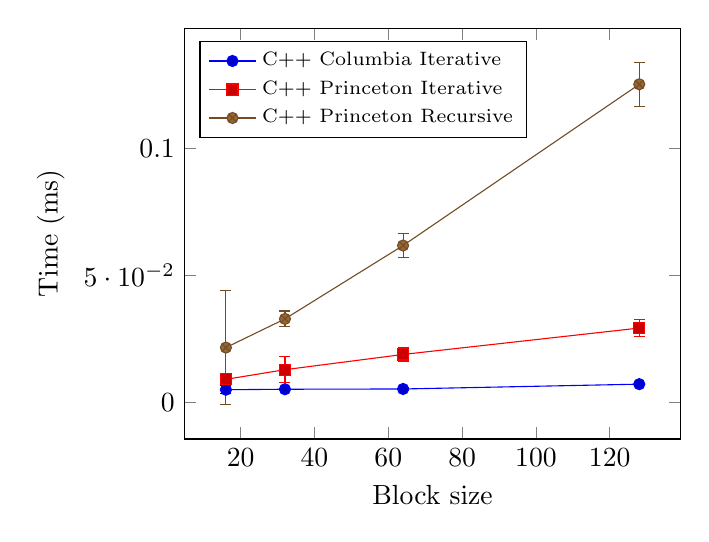
\begin{tikzpicture}
\begin{axis}[xlabel={Block size},ylabel={Time (ms)},width=0.65\linewidth,legend pos=north west,scaled y ticks = false,legend cell align=left,legend style={font=\scriptsize}]
\addplot+[error bars/.cd, y dir=both,y explicit] coordinates {
(16, 0.0049) +- (0.0015, 0.0015)
(32, 0.0051) +- (0.0002, 0.0002)
(64, 0.0052) +- (0.0005, 0.0005)
(128, 0.0071) +- (0.0003, 0.0003)
};
\addplot+[error bars/.cd, y dir=both,y explicit] coordinates {
(16, 0.0090) +- (0.0022, 0.0022)
(32, 0.0128) +- (0.0052, 0.0052)
(64, 0.0188) +- (0.0029, 0.0029)
(128, 0.0292) +- (0.0032, 0.0032)
};
\addplot+[error bars/.cd, y dir=both,y explicit] coordinates {
(16, 0.0215) +- (0.0225, 0.0225)
(32, 0.0328) +- (0.0031, 0.0031)
(64, 0.0617) +- (0.0047, 0.0047)
(128, 0.1252) +- (0.0086, 0.0086)
};
\legend{C++ Columbia Iterative , C++ Princeton Iterative , C++ Princeton Recursive}
\end{axis}
\end{tikzpicture}

%         &
%         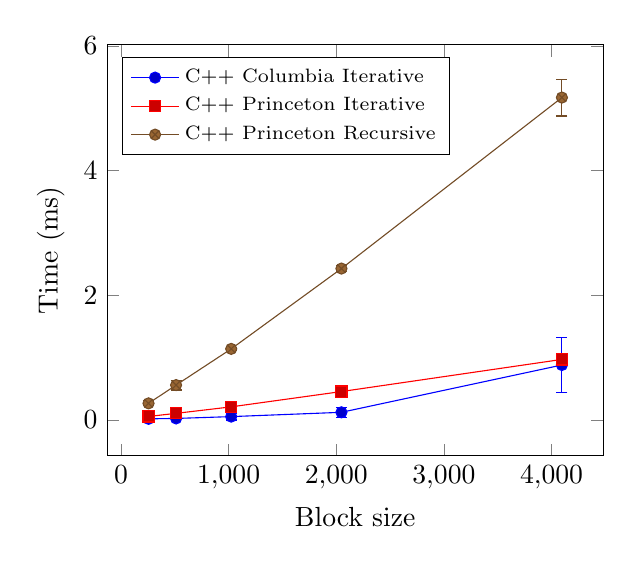
\begin{tikzpicture}
\begin{axis}[xlabel={Block size},ylabel={Time (ms)},width=0.65\linewidth,legend pos=north west,scaled y ticks = false,legend cell align=left,legend style={font=\scriptsize}]
\addplot+[error bars/.cd, y dir=both,y explicit] coordinates {
(256, 0.0160) +- (0.0408, 0.0408)
(512, 0.0223) +- (0.0032, 0.0032)
(1024, 0.0516) +- (0.0547, 0.0547)
(2048, 0.1206) +- (0.0787, 0.0787)
(4096, 0.8794) +- (0.4366, 0.4366)
};
\addplot+[error bars/.cd, y dir=both,y explicit] coordinates {
(256, 0.0541) +- (0.0048, 0.0048)
(512, 0.1038) +- (0.0056, 0.0056)
(1024, 0.2082) +- (0.0127, 0.0127)
(2048, 0.4536) +- (0.0536, 0.0536)
(4096, 0.9690) +- (0.0314, 0.0314)
};
\addplot+[error bars/.cd, y dir=both,y explicit] coordinates {
(256, 0.2642) +- (0.0405, 0.0405)
(512, 0.5573) +- (0.0791, 0.0791)
(1024, 1.1380) +- (0.0245, 0.0245)
(2048, 2.4265) +- (0.0476, 0.0476)
(4096, 5.1699) +- (0.2963, 0.2963)
};
\legend{C++ Columbia Iterative , C++ Princeton Iterative , C++ Princeton Recursive}
\end{axis}
\end{tikzpicture}

%         \\
%         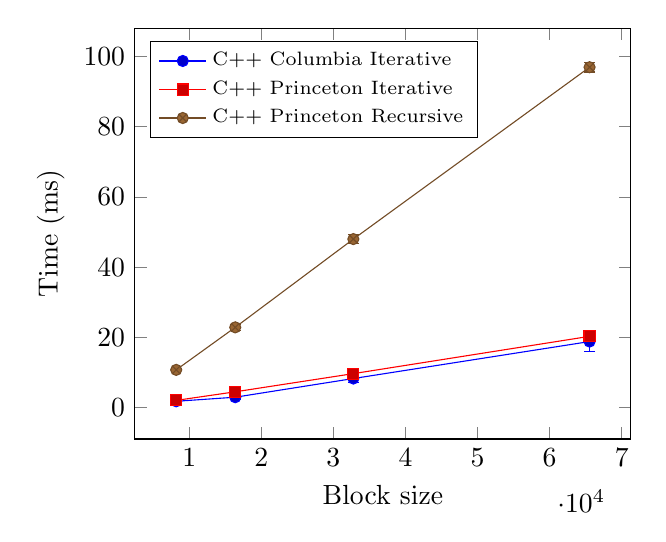
\begin{tikzpicture}
\begin{axis}[xlabel={Block size},ylabel={Time (ms)},width=0.65\linewidth,legend pos=north west,scaled y ticks = false,legend cell align=left,legend style={font=\scriptsize}]
\addplot+[error bars/.cd, y dir=both,y explicit] coordinates {
(8192, 1.8030) +- (0.9841, 0.9841)
(16384, 2.9629) +- (0.6687, 0.6687)
(32768, 8.2847) +- (1.2061, 1.2061)
(65536, 18.8158) +- (2.8032, 2.8032)
};
\addplot+[error bars/.cd, y dir=both,y explicit] coordinates {
(8192, 2.0605) +- (0.0561, 0.0561)
(16384, 4.5027) +- (0.1737, 0.1737)
(32768, 9.6797) +- (0.6568, 0.6568)
(65536, 20.3049) +- (1.7691, 1.7691)
};
\addplot+[error bars/.cd, y dir=both,y explicit] coordinates {
(8192, 10.7496) +- (0.2605, 0.2605)
(16384, 22.8640) +- (0.8917, 0.8917)
(32768, 48.0022) +- (1.2536, 1.2536)
(65536, 96.9572) +- (1.3564, 1.3564)
};
\legend{C++ Columbia Iterative , C++ Princeton Iterative , C++ Princeton Recursive}
\end{axis}
\end{tikzpicture}

%         &
%         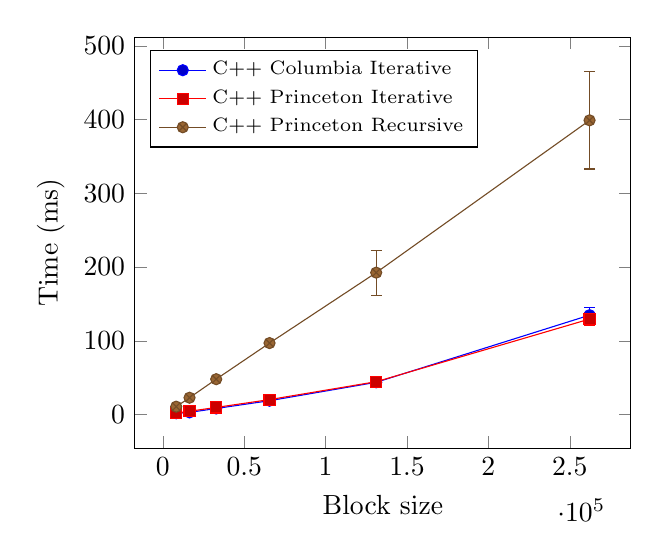
\begin{tikzpicture}
\begin{axis}[xlabel={Block size},ylabel={Time (ms)},width=0.65\linewidth,legend pos=north west,scaled y ticks = false,legend cell align=left,legend style={font=\scriptsize}]
\addplot+[error bars/.cd, y dir=both,y explicit] coordinates {
(8192, 1.8030) +- (0.9841, 0.9841)
(16384, 2.9629) +- (0.6687, 0.6687)
(32768, 8.2847) +- (1.2061, 1.2061)
(65536, 18.8158) +- (2.8032, 2.8032)
(131072, 43.7807) +- (6.4454, 6.4454)
(262144, 134.8093) +- (10.2633, 10.2633)
};
\addplot+[error bars/.cd, y dir=both,y explicit] coordinates {
(8192, 2.0605) +- (0.0561, 0.0561)
(16384, 4.5027) +- (0.1737, 0.1737)
(32768, 9.6797) +- (0.6568, 0.6568)
(65536, 20.3049) +- (1.7691, 1.7691)
(131072, 44.5770) +- (4.8859, 4.8859)
(262144, 129.5150) +- (9.2859, 9.2859)
};
\addplot+[error bars/.cd, y dir=both,y explicit] coordinates {
(8192, 10.7496) +- (0.2605, 0.2605)
(16384, 22.8640) +- (0.8917, 0.8917)
(32768, 48.0022) +- (1.2536, 1.2536)
(65536, 96.9572) +- (1.3564, 1.3564)
(131072, 192.4607) +- (30.4597, 30.4597)
(262144, 398.9698) +- (65.9217, 65.9217)
};
\legend{C++ Columbia Iterative , C++ Princeton Iterative , C++ Princeton Recursive}
\end{axis}
\end{tikzpicture}

%     \end{tabular}
%     \caption{\texttt{float} C++}
%     \label{fig:appendix:float:cpp:line}
% \end{table}

% \begin{figure}[H]
%     \centering
%     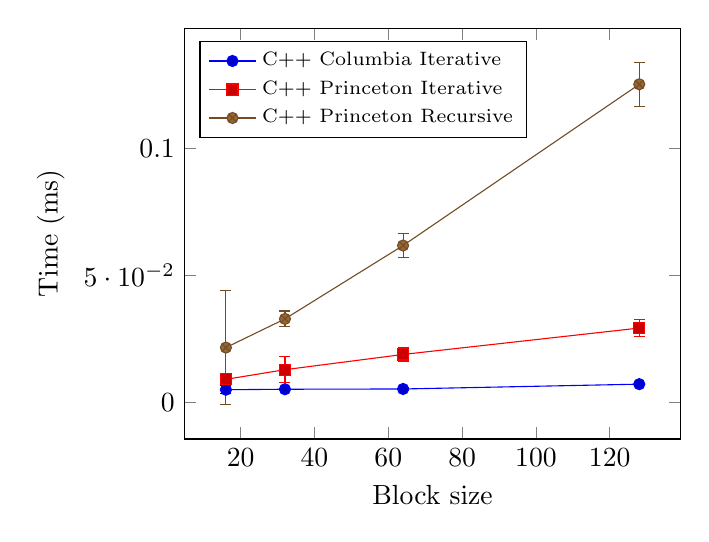
\begin{tikzpicture}
\begin{axis}[xlabel={Block size},ylabel={Time (ms)},width=0.65\linewidth,legend pos=north west,scaled y ticks = false,legend cell align=left,legend style={font=\scriptsize}]
\addplot+[error bars/.cd, y dir=both,y explicit] coordinates {
(16, 0.0049) +- (0.0015, 0.0015)
(32, 0.0051) +- (0.0002, 0.0002)
(64, 0.0052) +- (0.0005, 0.0005)
(128, 0.0071) +- (0.0003, 0.0003)
};
\addplot+[error bars/.cd, y dir=both,y explicit] coordinates {
(16, 0.0090) +- (0.0022, 0.0022)
(32, 0.0128) +- (0.0052, 0.0052)
(64, 0.0188) +- (0.0029, 0.0029)
(128, 0.0292) +- (0.0032, 0.0032)
};
\addplot+[error bars/.cd, y dir=both,y explicit] coordinates {
(16, 0.0215) +- (0.0225, 0.0225)
(32, 0.0328) +- (0.0031, 0.0031)
(64, 0.0617) +- (0.0047, 0.0047)
(128, 0.1252) +- (0.0086, 0.0086)
};
\legend{C++ Columbia Iterative , C++ Princeton Iterative , C++ Princeton Recursive}
\end{axis}
\end{tikzpicture}

%     \caption{\texttt{float} C++ small}
%     \label{fig:float:cpp:line:small}
% \end{figure}
% \begin{figure}[H]
%     \centering
%     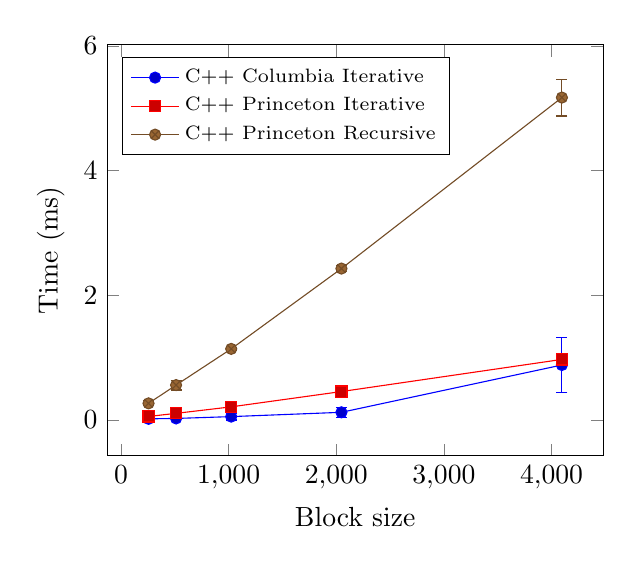
\begin{tikzpicture}
\begin{axis}[xlabel={Block size},ylabel={Time (ms)},width=0.65\linewidth,legend pos=north west,scaled y ticks = false,legend cell align=left,legend style={font=\scriptsize}]
\addplot+[error bars/.cd, y dir=both,y explicit] coordinates {
(256, 0.0160) +- (0.0408, 0.0408)
(512, 0.0223) +- (0.0032, 0.0032)
(1024, 0.0516) +- (0.0547, 0.0547)
(2048, 0.1206) +- (0.0787, 0.0787)
(4096, 0.8794) +- (0.4366, 0.4366)
};
\addplot+[error bars/.cd, y dir=both,y explicit] coordinates {
(256, 0.0541) +- (0.0048, 0.0048)
(512, 0.1038) +- (0.0056, 0.0056)
(1024, 0.2082) +- (0.0127, 0.0127)
(2048, 0.4536) +- (0.0536, 0.0536)
(4096, 0.9690) +- (0.0314, 0.0314)
};
\addplot+[error bars/.cd, y dir=both,y explicit] coordinates {
(256, 0.2642) +- (0.0405, 0.0405)
(512, 0.5573) +- (0.0791, 0.0791)
(1024, 1.1380) +- (0.0245, 0.0245)
(2048, 2.4265) +- (0.0476, 0.0476)
(4096, 5.1699) +- (0.2963, 0.2963)
};
\legend{C++ Columbia Iterative , C++ Princeton Iterative , C++ Princeton Recursive}
\end{axis}
\end{tikzpicture}

%     \caption{\texttt{float} C++ medium}
%     \label{fig:float:cpp:line:medium}
% \end{figure}
% \begin{figure}[H]
%     \centering
%     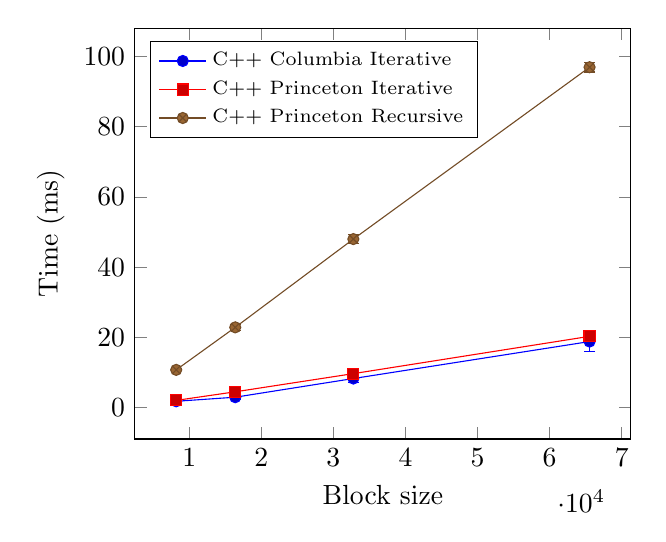
\begin{tikzpicture}
\begin{axis}[xlabel={Block size},ylabel={Time (ms)},width=0.65\linewidth,legend pos=north west,scaled y ticks = false,legend cell align=left,legend style={font=\scriptsize}]
\addplot+[error bars/.cd, y dir=both,y explicit] coordinates {
(8192, 1.8030) +- (0.9841, 0.9841)
(16384, 2.9629) +- (0.6687, 0.6687)
(32768, 8.2847) +- (1.2061, 1.2061)
(65536, 18.8158) +- (2.8032, 2.8032)
};
\addplot+[error bars/.cd, y dir=both,y explicit] coordinates {
(8192, 2.0605) +- (0.0561, 0.0561)
(16384, 4.5027) +- (0.1737, 0.1737)
(32768, 9.6797) +- (0.6568, 0.6568)
(65536, 20.3049) +- (1.7691, 1.7691)
};
\addplot+[error bars/.cd, y dir=both,y explicit] coordinates {
(8192, 10.7496) +- (0.2605, 0.2605)
(16384, 22.8640) +- (0.8917, 0.8917)
(32768, 48.0022) +- (1.2536, 1.2536)
(65536, 96.9572) +- (1.3564, 1.3564)
};
\legend{C++ Columbia Iterative , C++ Princeton Iterative , C++ Princeton Recursive}
\end{axis}
\end{tikzpicture}

%     \caption{\texttt{float} C++ large}
%     \label{fig:float:cpp:line:large}
% \end{figure}
% \begin{figure}[H]
%     \centering
%     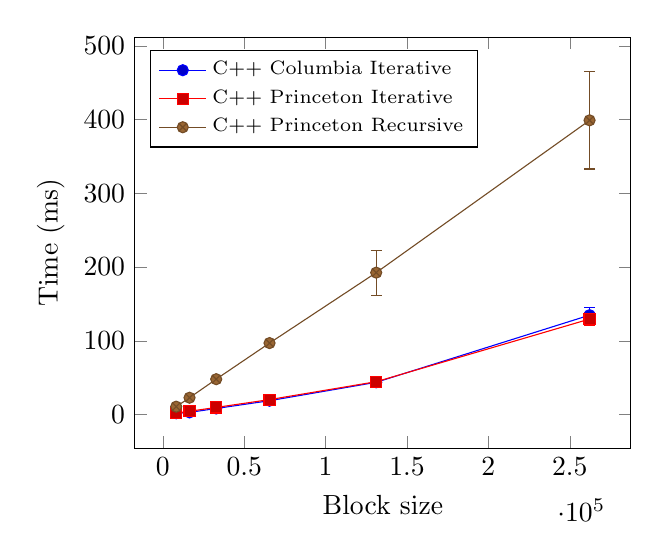
\begin{tikzpicture}
\begin{axis}[xlabel={Block size},ylabel={Time (ms)},width=0.65\linewidth,legend pos=north west,scaled y ticks = false,legend cell align=left,legend style={font=\scriptsize}]
\addplot+[error bars/.cd, y dir=both,y explicit] coordinates {
(8192, 1.8030) +- (0.9841, 0.9841)
(16384, 2.9629) +- (0.6687, 0.6687)
(32768, 8.2847) +- (1.2061, 1.2061)
(65536, 18.8158) +- (2.8032, 2.8032)
(131072, 43.7807) +- (6.4454, 6.4454)
(262144, 134.8093) +- (10.2633, 10.2633)
};
\addplot+[error bars/.cd, y dir=both,y explicit] coordinates {
(8192, 2.0605) +- (0.0561, 0.0561)
(16384, 4.5027) +- (0.1737, 0.1737)
(32768, 9.6797) +- (0.6568, 0.6568)
(65536, 20.3049) +- (1.7691, 1.7691)
(131072, 44.5770) +- (4.8859, 4.8859)
(262144, 129.5150) +- (9.2859, 9.2859)
};
\addplot+[error bars/.cd, y dir=both,y explicit] coordinates {
(8192, 10.7496) +- (0.2605, 0.2605)
(16384, 22.8640) +- (0.8917, 0.8917)
(32768, 48.0022) +- (1.2536, 1.2536)
(65536, 96.9572) +- (1.3564, 1.3564)
(131072, 192.4607) +- (30.4597, 30.4597)
(262144, 398.9698) +- (65.9217, 65.9217)
};
\legend{C++ Columbia Iterative , C++ Princeton Iterative , C++ Princeton Recursive}
\end{axis}
\end{tikzpicture}

%     \caption{\texttt{float} C++ extra}
%     \label{fig:float:cpp:line:extra}
% \end{figure}

\subsection{Java Float graphs}
%%==================================================================
%% Java Float graphs
%%==================================================================
% \begin{table}[H]
%     \centering
%     \begin{tabular}{cc}
%         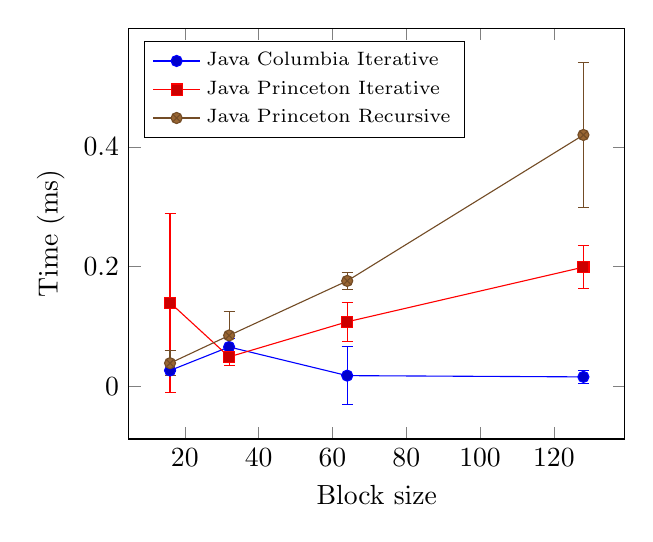
\begin{tikzpicture}
\begin{axis}[xlabel={Block size},ylabel={Time (ms)},width=0.65\linewidth,legend pos=north west,scaled y ticks = false,legend cell align=left,legend style={font=\scriptsize}]
\addplot+[error bars/.cd, y dir=both,y explicit] coordinates {
(16, 0.0265) +- (0.0011, 0.0011)
(32, 0.0658) +- (0.0148, 0.0148)
(64, 0.0179) +- (0.0486, 0.0486)
(128, 0.0158) +- (0.0105, 0.0105)
};
\addplot+[error bars/.cd, y dir=both,y explicit] coordinates {
(16, 0.1398) +- (0.1496, 0.1496)
(32, 0.0492) +- (0.0139, 0.0139)
(64, 0.1078) +- (0.0326, 0.0326)
(128, 0.1991) +- (0.0359, 0.0359)
};
\addplot+[error bars/.cd, y dir=both,y explicit] coordinates {
(16, 0.0387) +- (0.0210, 0.0210)
(32, 0.0850) +- (0.0396, 0.0396)
(64, 0.1761) +- (0.0136, 0.0136)
(128, 0.4199) +- (0.1211, 0.1211)
};
\legend{Java Columbia Iterative , Java Princeton Iterative , Java Princeton Recursive}
\end{axis}
\end{tikzpicture}

%         &
%         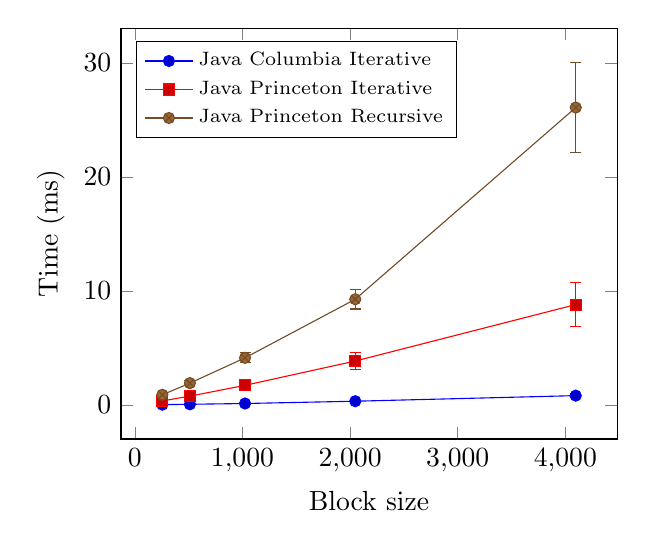
\begin{tikzpicture}
\begin{axis}[xlabel={Block size},ylabel={Time (ms)},width=0.65\linewidth,legend pos=north west,scaled y ticks = false,legend cell align=left,legend style={font=\scriptsize}]
\addplot+[error bars/.cd, y dir=both,y explicit] coordinates {
(256, 0.0290) +- (0.0075, 0.0075)
(512, 0.0603) +- (0.0073, 0.0073)
(1024, 0.1289) +- (0.0141, 0.0141)
(2048, 0.3302) +- (0.0926, 0.0926)
(4096, 0.8200) +- (0.1385, 0.1385)
};
\addplot+[error bars/.cd, y dir=both,y explicit] coordinates {
(256, 0.3547) +- (0.1008, 0.1008)
(512, 0.7740) +- (0.1657, 0.1657)
(1024, 1.7228) +- (0.2675, 0.2675)
(2048, 3.8546) +- (0.7268, 0.7268)
(4096, 8.8053) +- (1.9485, 1.9485)
};
\addplot+[error bars/.cd, y dir=both,y explicit] coordinates {
(256, 0.8938) +- (0.1489, 0.1489)
(512, 1.9155) +- (0.2226, 0.2226)
(1024, 4.1350) +- (0.4424, 0.4424)
(2048, 9.2740) +- (0.8540, 0.8540)
(4096, 26.0912) +- (3.9554, 3.9554)
};
\legend{Java Columbia Iterative , Java Princeton Iterative , Java Princeton Recursive}
\end{axis}
\end{tikzpicture}

%         \\
%         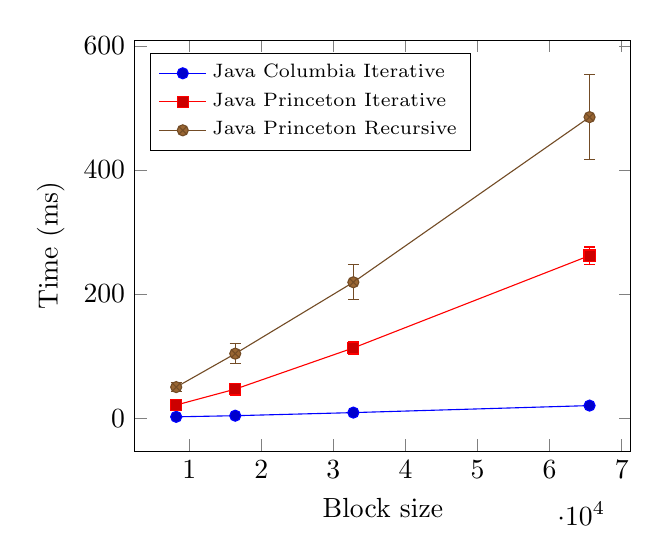
\begin{tikzpicture}
\begin{axis}[xlabel={Block size},ylabel={Time (ms)},width=0.65\linewidth,legend pos=north west,scaled y ticks = false,legend cell align=left,legend style={font=\scriptsize}]
\addplot+[error bars/.cd, y dir=both,y explicit] coordinates {
(8192, 2.1766) +- (0.3256, 0.3256)
(16384, 3.9995) +- (0.4596, 0.4596)
(32768, 8.9846) +- (1.3089, 1.3089)
(65536, 20.2833) +- (2.4423, 2.4423)
};
\addplot+[error bars/.cd, y dir=both,y explicit] coordinates {
(8192, 21.1757) +- (4.9079, 4.9079)
(16384, 46.8150) +- (9.6619, 9.6619)
(32768, 113.1953) +- (11.0218, 11.0218)
(65536, 261.9954) +- (13.8293, 13.8293)
};
\addplot+[error bars/.cd, y dir=both,y explicit] coordinates {
(8192, 50.0776) +- (7.5896, 7.5896)
(16384, 103.9682) +- (15.7929, 15.7929)
(32768, 219.0208) +- (28.3890, 28.3890)
(65536, 485.1020) +- (68.2330, 68.2330)
};
\legend{Java Columbia Iterative , Java Princeton Iterative , Java Princeton Recursive}
\end{axis}
\end{tikzpicture}

%         &
%         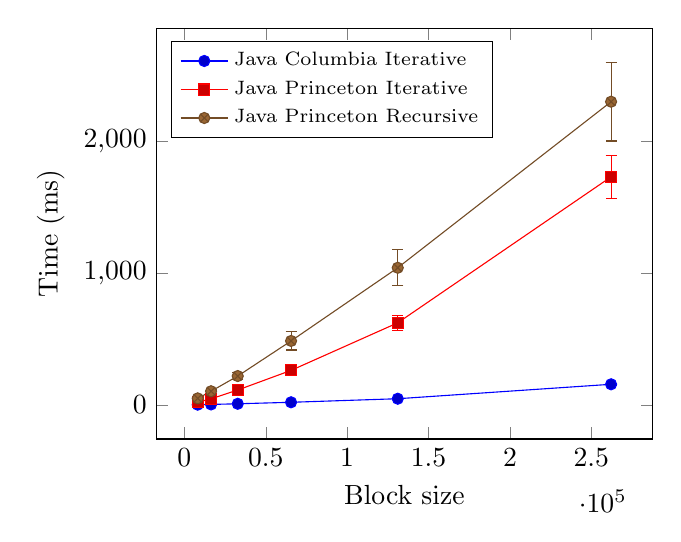
\begin{tikzpicture}
\begin{axis}[xlabel={Block size},ylabel={Time (ms)},width=0.65\linewidth,legend pos=north west,scaled y ticks = false,legend cell align=left,legend style={font=\scriptsize}]
\addplot+[error bars/.cd, y dir=both,y explicit] coordinates {
(8192, 2.1766) +- (0.3256, 0.3256)
(16384, 3.9995) +- (0.4596, 0.4596)
(32768, 8.9846) +- (1.3089, 1.3089)
(65536, 20.2833) +- (2.4423, 2.4423)
(131072, 47.2950) +- (6.6700, 6.6700)
(262144, 156.7135) +- (6.0892, 6.0892)
};
\addplot+[error bars/.cd, y dir=both,y explicit] coordinates {
(8192, 21.1757) +- (4.9079, 4.9079)
(16384, 46.8150) +- (9.6619, 9.6619)
(32768, 113.1953) +- (11.0218, 11.0218)
(65536, 261.9954) +- (13.8293, 13.8293)
(131072, 622.4328) +- (57.9001, 57.9001)
(262144, 1728.4640) +- (161.0712, 161.0712)
};
\addplot+[error bars/.cd, y dir=both,y explicit] coordinates {
(8192, 50.0776) +- (7.5896, 7.5896)
(16384, 103.9682) +- (15.7929, 15.7929)
(32768, 219.0208) +- (28.3890, 28.3890)
(65536, 485.1020) +- (68.2330, 68.2330)
(131072, 1039.4937) +- (137.6356, 137.6356)
(262144, 2297.8011) +- (297.4241, 297.4241)
};
\legend{Java Columbia Iterative , Java Princeton Iterative , Java Princeton Recursive}
\end{axis}
\end{tikzpicture}

%     \end{tabular}
%     \caption{\texttt{float} Java}
%     \label{fig:appendix:float:java:line}
% \end{table}

% \begin{figure}[H]
%     \centering
%     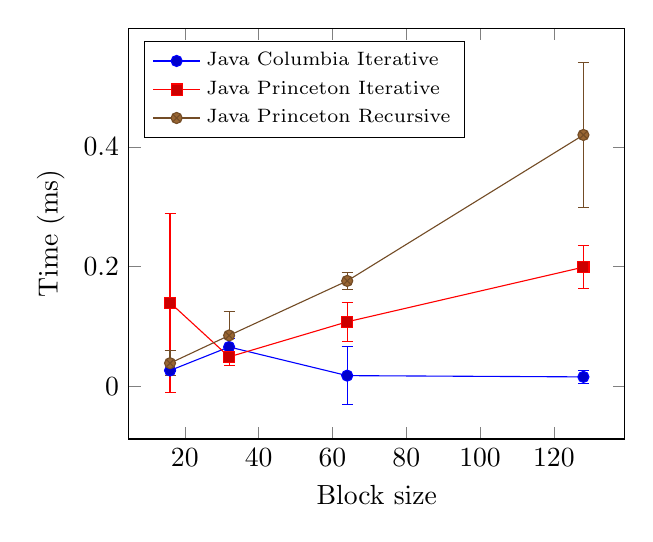
\begin{tikzpicture}
\begin{axis}[xlabel={Block size},ylabel={Time (ms)},width=0.65\linewidth,legend pos=north west,scaled y ticks = false,legend cell align=left,legend style={font=\scriptsize}]
\addplot+[error bars/.cd, y dir=both,y explicit] coordinates {
(16, 0.0265) +- (0.0011, 0.0011)
(32, 0.0658) +- (0.0148, 0.0148)
(64, 0.0179) +- (0.0486, 0.0486)
(128, 0.0158) +- (0.0105, 0.0105)
};
\addplot+[error bars/.cd, y dir=both,y explicit] coordinates {
(16, 0.1398) +- (0.1496, 0.1496)
(32, 0.0492) +- (0.0139, 0.0139)
(64, 0.1078) +- (0.0326, 0.0326)
(128, 0.1991) +- (0.0359, 0.0359)
};
\addplot+[error bars/.cd, y dir=both,y explicit] coordinates {
(16, 0.0387) +- (0.0210, 0.0210)
(32, 0.0850) +- (0.0396, 0.0396)
(64, 0.1761) +- (0.0136, 0.0136)
(128, 0.4199) +- (0.1211, 0.1211)
};
\legend{Java Columbia Iterative , Java Princeton Iterative , Java Princeton Recursive}
\end{axis}
\end{tikzpicture}

%     \caption{\texttt{float} Java small}
%     \label{fig:float:java:line:small}
% \end{figure}
% \begin{figure}[H]
%     \centering
%     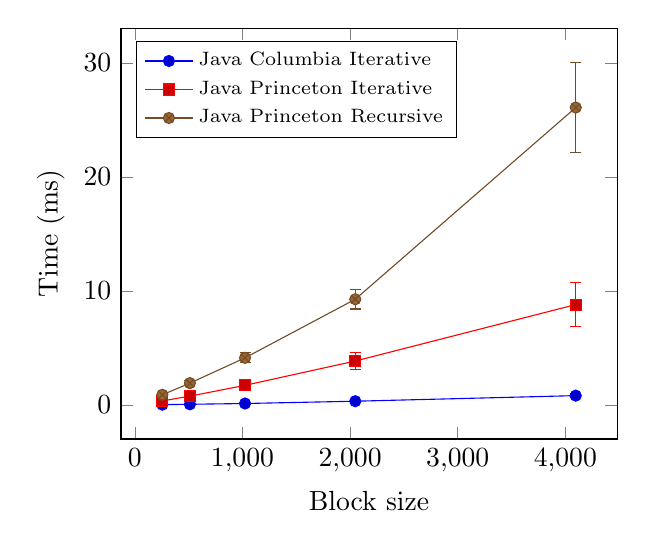
\begin{tikzpicture}
\begin{axis}[xlabel={Block size},ylabel={Time (ms)},width=0.65\linewidth,legend pos=north west,scaled y ticks = false,legend cell align=left,legend style={font=\scriptsize}]
\addplot+[error bars/.cd, y dir=both,y explicit] coordinates {
(256, 0.0290) +- (0.0075, 0.0075)
(512, 0.0603) +- (0.0073, 0.0073)
(1024, 0.1289) +- (0.0141, 0.0141)
(2048, 0.3302) +- (0.0926, 0.0926)
(4096, 0.8200) +- (0.1385, 0.1385)
};
\addplot+[error bars/.cd, y dir=both,y explicit] coordinates {
(256, 0.3547) +- (0.1008, 0.1008)
(512, 0.7740) +- (0.1657, 0.1657)
(1024, 1.7228) +- (0.2675, 0.2675)
(2048, 3.8546) +- (0.7268, 0.7268)
(4096, 8.8053) +- (1.9485, 1.9485)
};
\addplot+[error bars/.cd, y dir=both,y explicit] coordinates {
(256, 0.8938) +- (0.1489, 0.1489)
(512, 1.9155) +- (0.2226, 0.2226)
(1024, 4.1350) +- (0.4424, 0.4424)
(2048, 9.2740) +- (0.8540, 0.8540)
(4096, 26.0912) +- (3.9554, 3.9554)
};
\legend{Java Columbia Iterative , Java Princeton Iterative , Java Princeton Recursive}
\end{axis}
\end{tikzpicture}

%     \caption{\texttt{float} Java medium}
%     \label{fig:float:java:line:medium}
% \end{figure}
% \begin{figure}[H]
%     \centering
%     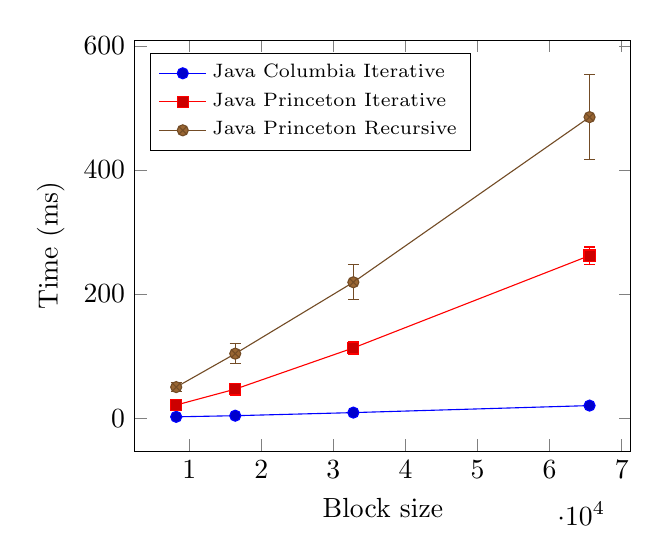
\begin{tikzpicture}
\begin{axis}[xlabel={Block size},ylabel={Time (ms)},width=0.65\linewidth,legend pos=north west,scaled y ticks = false,legend cell align=left,legend style={font=\scriptsize}]
\addplot+[error bars/.cd, y dir=both,y explicit] coordinates {
(8192, 2.1766) +- (0.3256, 0.3256)
(16384, 3.9995) +- (0.4596, 0.4596)
(32768, 8.9846) +- (1.3089, 1.3089)
(65536, 20.2833) +- (2.4423, 2.4423)
};
\addplot+[error bars/.cd, y dir=both,y explicit] coordinates {
(8192, 21.1757) +- (4.9079, 4.9079)
(16384, 46.8150) +- (9.6619, 9.6619)
(32768, 113.1953) +- (11.0218, 11.0218)
(65536, 261.9954) +- (13.8293, 13.8293)
};
\addplot+[error bars/.cd, y dir=both,y explicit] coordinates {
(8192, 50.0776) +- (7.5896, 7.5896)
(16384, 103.9682) +- (15.7929, 15.7929)
(32768, 219.0208) +- (28.3890, 28.3890)
(65536, 485.1020) +- (68.2330, 68.2330)
};
\legend{Java Columbia Iterative , Java Princeton Iterative , Java Princeton Recursive}
\end{axis}
\end{tikzpicture}

%     \caption{\texttt{float} Java large}
%     \label{fig:float:java:line:large}
% \end{figure}
% \begin{figure}[H]
%     \centering
%     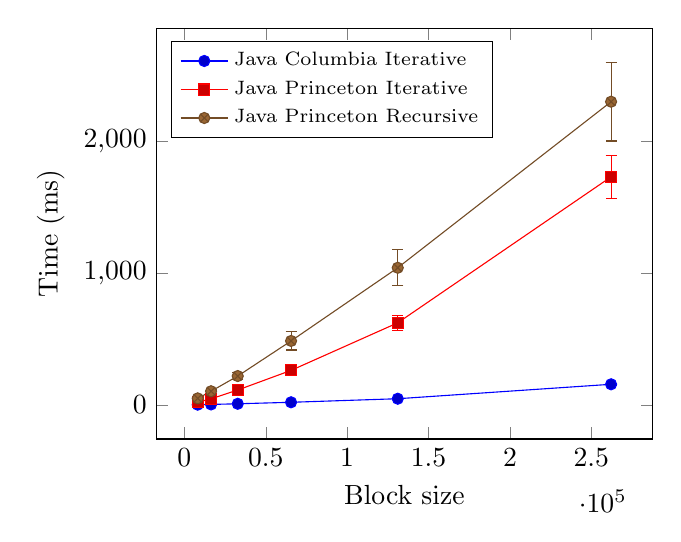
\begin{tikzpicture}
\begin{axis}[xlabel={Block size},ylabel={Time (ms)},width=0.65\linewidth,legend pos=north west,scaled y ticks = false,legend cell align=left,legend style={font=\scriptsize}]
\addplot+[error bars/.cd, y dir=both,y explicit] coordinates {
(8192, 2.1766) +- (0.3256, 0.3256)
(16384, 3.9995) +- (0.4596, 0.4596)
(32768, 8.9846) +- (1.3089, 1.3089)
(65536, 20.2833) +- (2.4423, 2.4423)
(131072, 47.2950) +- (6.6700, 6.6700)
(262144, 156.7135) +- (6.0892, 6.0892)
};
\addplot+[error bars/.cd, y dir=both,y explicit] coordinates {
(8192, 21.1757) +- (4.9079, 4.9079)
(16384, 46.8150) +- (9.6619, 9.6619)
(32768, 113.1953) +- (11.0218, 11.0218)
(65536, 261.9954) +- (13.8293, 13.8293)
(131072, 622.4328) +- (57.9001, 57.9001)
(262144, 1728.4640) +- (161.0712, 161.0712)
};
\addplot+[error bars/.cd, y dir=both,y explicit] coordinates {
(8192, 50.0776) +- (7.5896, 7.5896)
(16384, 103.9682) +- (15.7929, 15.7929)
(32768, 219.0208) +- (28.3890, 28.3890)
(65536, 485.1020) +- (68.2330, 68.2330)
(131072, 1039.4937) +- (137.6356, 137.6356)
(262144, 2297.8011) +- (297.4241, 297.4241)
};
\legend{Java Columbia Iterative , Java Princeton Iterative , Java Princeton Recursive}
\end{axis}
\end{tikzpicture}

%     \caption{\texttt{float} Java extra}
%     \label{fig:float:java:line:extra}
% \end{figure}




%
% \begin{table}[H]
%     \centering
%     \label{tab:common:table:cpp}
%     \caption{Common table for C++ tests, Time (ms)}
%     \resizebox{\columnwidth}{!}{
%         \begin{tabular}{|l|c|c|c|c|c|}\hline
\textbf{Block size}  & \textbf{Columbia converted Iterative} & \textbf{Columbia optimized Iterative} & \textbf{KISS} & \textbf{Princeton converted Iterative} & \textbf{Princeton converted Recursive}\\\hline
\textbf{16}  & 0.0225 $\pm$ 0.0033 & 0.0198 $\pm$ 0.0025 & 0.0195 $\pm$ 0.0067 & 0.0342 $\pm$ 0.0053 & 0.0612 $\pm$ 0.0065\\\hline
\textbf{32}  & 0.0322 $\pm$ 0.0025 & 0.0322 $\pm$ 0.0031 & 0.0239 $\pm$ 0.0031 & 0.0545 $\pm$ 0.0043 & 0.1085 $\pm$ 0.0020\\\hline
\textbf{64}  & 0.0525 $\pm$ 0.0014 & 0.0524 $\pm$ 0.0012 & 0.0338 $\pm$ 0.0020 & 0.0847 $\pm$ 0.0059 & 0.2148 $\pm$ 0.0024\\\hline
\textbf{128}  & 0.1025 $\pm$ 0.0033 & 0.0814 $\pm$ 0.0127 & 0.0629 $\pm$ 0.0084 & 0.1328 $\pm$ 0.0029 & 0.4517 $\pm$ 0.0057\\\hline
\textbf{256}  & 0.0925 $\pm$ 0.0178 & 0.0822 $\pm$ 0.0039 & 0.1158 $\pm$ 0.0035 & 0.2807 $\pm$ 0.0073 & 0.9139 $\pm$ 0.0067\\\hline
\textbf{512}  & 0.1709 $\pm$ 0.0267 & 0.1744 $\pm$ 0.0308 & 0.2109 $\pm$ 0.0049 & 0.5486 $\pm$ 0.0253 & 1.9142 $\pm$ 0.0102\\\hline
\textbf{1024}  & 0.3656 $\pm$ 0.0284 & 0.3397 $\pm$ 0.0108 & 0.4072 $\pm$ 0.0086 & 1.1691 $\pm$ 0.0172 & 4.0665 $\pm$ 0.0127\\\hline
\textbf{2048}  & 0.9177 $\pm$ 0.0541 & 0.7402 $\pm$ 0.0190 & 0.8635 $\pm$ 0.0243 & 2.4714 $\pm$ 0.0188 & 8.7235 $\pm$ 0.0725\\\hline
\textbf{4096}  & 1.6737 $\pm$ 0.0461 & 1.9889 $\pm$ 0.0982 & 1.9558 $\pm$ 0.1347 & 5.3867 $\pm$ 0.1000 & 18.3487 $\pm$ 0.1235\\\hline
\textbf{8192}  & 3.7768 $\pm$ 0.1838 & 3.8584 $\pm$ 0.2236 & 3.8499 $\pm$ 0.1603 & 11.7050 $\pm$ 0.5076 & 38.4780 $\pm$ 0.6441\\\hline
\textbf{16384}  & 8.2947 $\pm$ 0.3759 & 8.5556 $\pm$ 0.5672 & 7.8854 $\pm$ 0.2775 & 24.3807 $\pm$ 0.5902 & 80.4920 $\pm$ 0.8228\\\hline
\textbf{32768}  & 19.1886 $\pm$ 1.1809 & 18.5907 $\pm$ 0.9959 & 17.6197 $\pm$ 0.5490 & 52.3713 $\pm$ 1.1313 & 167.3867 $\pm$ 1.5300\\\hline
\textbf{65536} & 42.8520 $\pm$ 1.4120 & 44.2337 $\pm$ 2.4361 & 38.3601 $\pm$ 0.7332 & 112.4273 $\pm$ 1.1197 & 346.7600 $\pm$ 1.9190\\\hline
\end{tabular}

%     }
% \end{table}
%
% \begin{table}[H]
%     \centering
%     \label{tab:common:table:java}
%     \caption{Common table for Java tests, Time (ms)}
%     \resizebox{\columnwidth}{!}{
%         \begin{tabular}{|l|c|c|c|}\hline
\textbf{Block size}  & \textbf{Columbia Iterative} & \textbf{Princeton Iterative} & \textbf{Princeton Recursive}\\\hline
\textbf{16}  & 0.0210 $\pm$ 0.0008 & 0.1738 $\pm$ 0.0368 & 0.2730 $\pm$ 0.0708\\\hline
\textbf{32}  & 0.0429 $\pm$ 0.0018 & 0.0571 $\pm$ 0.0071 & 0.3983 $\pm$ 0.0568\\\hline
\textbf{64}  & 0.0906 $\pm$ 0.0010 & 0.0916 $\pm$ 0.0073 & 0.2104 $\pm$ 0.0402\\\hline
\textbf{128}  & 0.2233 $\pm$ 0.0382 & 0.2353 $\pm$ 0.0339 & 0.3204 $\pm$ 0.0425\\\hline
\textbf{256}  & 0.0372 $\pm$ 0.0022 & 0.4380 $\pm$ 0.0316 & 0.7415 $\pm$ 0.0431\\\hline
\textbf{512}  & 0.0754 $\pm$ 0.0029 & 0.9865 $\pm$ 0.0672 & 1.7743 $\pm$ 0.1944\\\hline
\textbf{1024}  & 0.1507 $\pm$ 0.0059 & 2.0255 $\pm$ 0.0933 & 3.5339 $\pm$ 0.2466\\\hline
\textbf{2048}  & 0.4299 $\pm$ 0.0312 & 4.5366 $\pm$ 0.3038 & 8.2740 $\pm$ 0.6905\\\hline
\textbf{4096}  & 0.9984 $\pm$ 0.0915 & 10.6191 $\pm$ 0.8679 & 17.9445 $\pm$ 0.9022\\\hline
\textbf{8192}  & 2.3125 $\pm$ 0.2709 & 27.5617 $\pm$ 1.9755 & 37.6118 $\pm$ 1.5008\\\hline
\textbf{16384}  & 4.8597 $\pm$ 0.4114 & 62.6869 $\pm$ 1.7191 & 80.1848 $\pm$ 1.9414\\\hline
\textbf{32768}  & 11.2535 $\pm$ 0.9718 & 155.5247 $\pm$ 2.7411 & 172.5062 $\pm$ 2.2489\\\hline
\textbf{65536} & 26.3906 $\pm$ 2.1662 & 366.0557 $\pm$ 2.8910 & 366.6833 $\pm$ 3.3610\\\hline
\end{tabular}

%     }
% \end{table}
%
% \begin{table}[H]
%     \centering
%     \label{tab:jni:convert}
%     \caption{JNI convert, Time (textmu s)}
%     \input{Data/results/JNI/Benchmark_convert.tex}
% \end{table}
%
% \begin{table}[H]
%     \centering
%     \label{tab:jni:no:params}
%     \caption{JNI no parameters, Time (textmu s)}
%     \input{Data/results/JNI/Benchmark_no_params.tex}
% \end{table}
%
% \begin{table}[H]
%     \centering
%     \label{tab:jni:vector}
%     \caption{JNI convert, Time (textmu s)}
%     \input{Data/results/JNI/Benchmark_vector.tex}
% \end{table}
%
% \begin{table}[H]
%     \centering
%     \label{tab:java:princeton:iterative}
%     \caption{Java Princeton Iterative, Time (ms)}
%     /home/algo/Skola/Exjobb/Data/results/FFT/Java_Princeton_Iterative_N_30.tex
% \end{table}
%
% \begin{table}[H]
%     \centering
%     \label{tab:java:princeton:recursive}
%     \caption{Java Princeton Recursive, Time (ms)}
%     /home/algo/Skola/Exjobb/Data/results/FFT/Java_Princeton_Recursive_N_30.tex
% \end{table}
%
% \begin{table}[H]
%     \centering
%     \label{tab:java:columbia:iterative}
%     \caption{Java Columbia Iterative, Time (ms)}
%     /home/algo/Skola/Exjobb/Data/results/FFT/Java_Columbia_Iterative_N_30.tex
% \end{table}
%
% \begin{table}[H]
%     \centering
%     \label{tab:cpp:princeton:iterative}
%     \caption{C++ Princeton Iterative, Time (ms)}
%     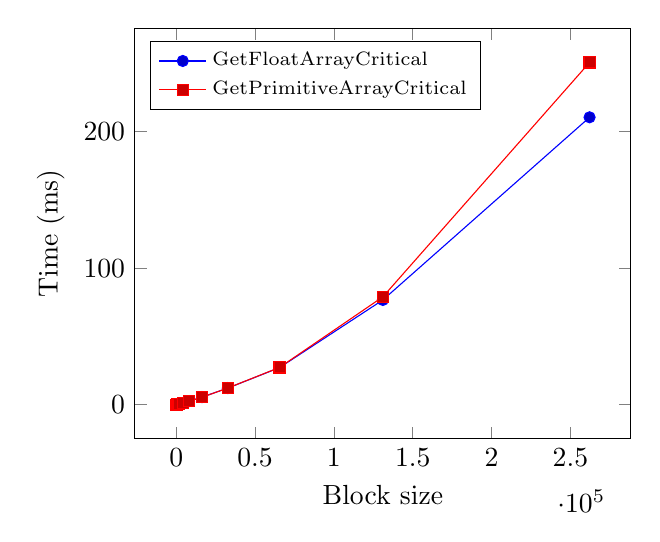
\begin{tikzpicture}
\begin{axis}[xlabel={Block size},ylabel={Time (ms)},width=0.65\linewidth,legend pos=north west,scaled y ticks = false,legend cell align=left,legend style={font=\scriptsize}]
\addplot coordinates {
(16, 0.0083)
(32, 0.0124)
(64, 0.0201)
(128, 0.0348)
(256, 0.0651)
(512, 0.1275)
(1024, 0.2659)
(2048, 0.5235)
(4096, 1.1475)
(8192, 2.6441)
(16384, 5.5785)
(32768, 12.1775)
(65536, 27.1549)
(131072, 76.6735)
(262144, 210.3414)
};
\addplot coordinates {
(16, 0.0097)
(32, 0.0132)
(64, 0.0214)
(128, 0.0342)
(256, 0.0627)
(512, 0.1225)
(1024, 0.2744)
(2048, 0.5257)
(4096, 1.1701)
(8192, 2.5845)
(16384, 5.4518)
(32768, 12.2266)
(65536, 27.2805)
(131072, 78.9501)
(262144, 250.4870)
};
\legend{GetFloatArrayCritical, GetPrimitiveArrayCritical}
\end{axis}
\end{tikzpicture}

% \end{table}
%
% \begin{table}[H]
%     \centering
%     \label{tab:cpp:princeton:recursive}
%     \caption{C++ Princeton Recursive, Time (ms)}
%     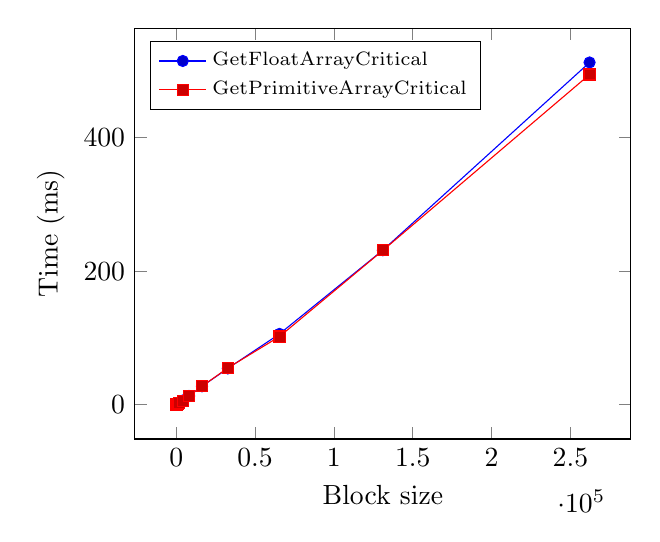
\begin{tikzpicture}
\begin{axis}[xlabel={Block size},ylabel={Time (ms)},width=0.65\linewidth,legend pos=north west,scaled y ticks = false,legend cell align=left,legend style={font=\scriptsize}]
\addplot coordinates {
(16, 0.0187)
(32, 0.0347)
(64, 0.0709)
(128, 0.1447)
(256, 0.3014)
(512, 0.6505)
(1024, 1.3689)
(2048, 2.9279)
(4096, 6.2499)
(8192, 13.1419)
(16384, 27.7314)
(32768, 54.4151)
(65536, 106.1420)
(131072, 231.5323)
(262144, 512.7674)
};
\addplot coordinates {
(16, 0.0202)
(32, 0.0368)
(64, 0.0705)
(128, 0.1434)
(256, 0.2978)
(512, 0.6379)
(1024, 1.3437)
(2048, 2.8773)
(4096, 6.1206)
(8192, 13.2345)
(16384, 27.6080)
(32768, 55.1227)
(65536, 102.1585)
(131072, 231.2663)
(262144, 494.7038)
};
\legend{GetFloatArrayCritical, GetPrimitiveArrayCritical}
\end{axis}
\end{tikzpicture}

% \end{table}
%
% \begin{table}[H]
%     \centering
%     \label{tab:cpp:columbia:iterative}
%     \caption{C++ Columbia Iterative, Time (ms)}
%     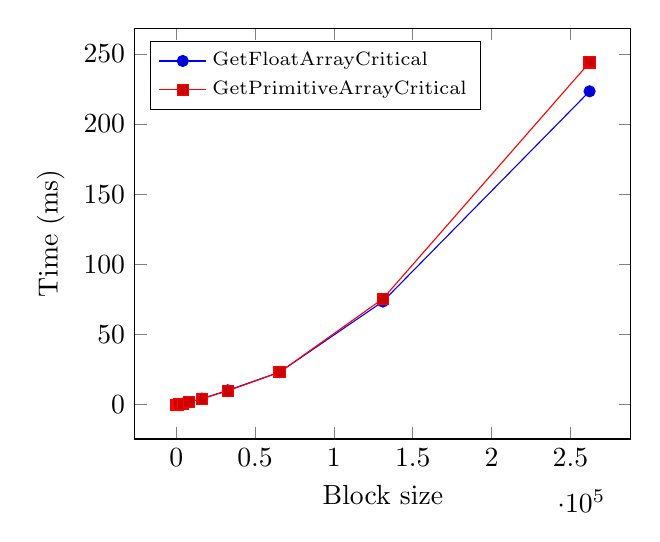
\begin{tikzpicture}
\begin{axis}[xlabel={Block size},ylabel={Time (ms)},width=0.65\linewidth,legend pos=north west,scaled y ticks = false,legend cell align=left,legend style={font=\scriptsize}]
\addplot coordinates {
(16, 0.0057)
(32, 0.0070)
(64, 0.0092)
(128, 0.0136)
(256, 0.0222)
(512, 0.0418)
(1024, 0.0970)
(2048, 0.2761)
(4096, 0.7818)
(8192, 1.8794)
(16384, 4.3304)
(32768, 10.2608)
(65536, 23.1917)
(131072, 73.5225)
(262144, 223.3088)
};
\addplot coordinates {
(16, 0.0072)
(32, 0.0086)
(64, 0.0083)
(128, 0.0115)
(256, 0.0200)
(512, 0.0366)
(1024, 0.0773)
(2048, 0.2604)
(4096, 0.7974)
(8192, 1.9326)
(16384, 4.2789)
(32768, 9.9388)
(65536, 23.1031)
(131072, 75.4942)
(262144, 243.8496)
};
\legend{GetFloatArrayCritical, GetPrimitiveArrayCritical}
\end{axis}
\end{tikzpicture}

% \end{table}
%
% \begin{table}[H]
%     \centering
%     \label{tab:cpp:kiss}
%     \caption{C++ KISS, Time (ms)}
%     /home/algo/Skola/Exjobb/Data/results/FFT/CPP_KISS_N_30.tex
% \end{table}
% \begin{table}
%     \centering
%     \label{tab:cpp:columbia:iterative:optimized}
%     \caption{C++ Columbia Iterative Optimized, Time (ms)}
%     \input{Data/results/FFT/CPP_Columbia_optimized.tex}
% \end{table}

% \begin{table}
%     \centering
%     \label{fig:java:columbia:iterative:optimized}
%     \caption{Label here}
%     \input{Data/results/FFT/Java_Columbia_optimized_Iterative.tex}
% \end{table}

% \section{Bar charts}

% \begin{figure}
%     \centering
%     \input{Data/results/FFT/Java_Princeton_Recursive_barchart.tex}
%     \label{fig:java:princeton:recursive:barchart}
%     \caption{Java Princeton Recursive bar chart}
% \end{figure}

\section{ARR}

\begin{table}[H]
    \centering
    \caption{Common table for ARR C++ tests, Time(ms)}
    \label{tab:appendix:common:arr}
    \rotatebox{90}{
        \resizebox{\columnwidth}{!}{
            \rowcolors{1}{}{lightgray}
\begin{tabular}{lrrrrrrrrr}\toprule
\textbf{Block size}  & \textbf{Columbia Iterative} & \textbf{Float Columbia Iterative} & \textbf{Float Princeton Iterative} & \textbf{Float Princeton Recursive} & \textbf{KISS} & \textbf{NEON Iterative} & \textbf{NEON Recursive} & \textbf{Princeton Iterative} & \textbf{Princeton Recursive}\\\midrule
\textbf{16}  & 0.005 $\pm$ 0.0004 & 0.003 $\pm$ 0.0002 & 0.007 $\pm$ 0.0004 & 0.022 $\pm$ 0.0090 & 0.005 $\pm$ 0.0010 & 0.004 $\pm$ 0.0010 & 0.007 $\pm$ 0.0006 & 0.008 $\pm$ 0.0008 & 0.018 $\pm$ 0.0006\\
\textbf{32}  & 0.007 $\pm$ 0.0002 & 0.004 $\pm$ 0.0008 & 0.011 $\pm$ 0.0008 & 0.031 $\pm$ 0.0006 & 0.006 $\pm$ 0.0002 & 0.004 $\pm$ 0.0008 & 0.010 $\pm$ 0.0004 & 0.012 $\pm$ 0.0010 & 0.034 $\pm$ 0.0002\\
\textbf{64}  & 0.009 $\pm$ 0.0002 & 0.005 $\pm$ 0.0001 & 0.016 $\pm$ 0.0002 & 0.061 $\pm$ 0.0002 & 0.007 $\pm$ 0.0002 & 0.005 $\pm$ 0.0002 & 0.016 $\pm$ 0.0004 & 0.020 $\pm$ 0.0006 & 0.070 $\pm$ 0.0022\\
\textbf{128}  & 0.013 $\pm$ 0.0010 & 0.007 $\pm$ 0.0002 & 0.031 $\pm$ 0.0010 & 0.126 $\pm$ 0.0008 & 0.013 $\pm$ 0.0004 & 0.008 $\pm$ 0.0010 & 0.028 $\pm$ 0.0012 & 0.034 $\pm$ 0.0004 & 0.144 $\pm$ 0.0016\\
\textbf{256}  & 0.022 $\pm$ 0.0022 & 0.012 $\pm$ 0.0002 & 0.057 $\pm$ 0.0010 & 0.263 $\pm$ 0.0024 & 0.021 $\pm$ 0.0020 & 0.013 $\pm$ 0.0004 & 0.050 $\pm$ 0.0020 & 0.065 $\pm$ 0.0010 & 0.301 $\pm$ 0.0024\\
\textbf{512}  & 0.041 $\pm$ 0.0010 & 0.024 $\pm$ 0.0016 & 0.113 $\pm$ 0.0114 & 0.554 $\pm$ 0.0108 & 0.047 $\pm$ 0.0024 & 0.031 $\pm$ 0.0004 & 0.103 $\pm$ 0.0088 & 0.127 $\pm$ 0.0022 & 0.650 $\pm$ 0.0037\\
\textbf{1024}  & 0.097 $\pm$ 0.0100 & 0.051 $\pm$ 0.0012 & 0.218 $\pm$ 0.0024 & 1.166 $\pm$ 0.0057 & 0.088 $\pm$ 0.0120 & 0.066 $\pm$ 0.0106 & 0.191 $\pm$ 0.0025 & 0.265 $\pm$ 0.0027 & 1.368 $\pm$ 0.0122\\
\textbf{2048}  & 0.276 $\pm$ 0.0102 & 0.133 $\pm$ 0.0427 & 0.418 $\pm$ 0.0031 & 2.429 $\pm$ 0.0065 & 0.196 $\pm$ 0.0045 & 0.132 $\pm$ 0.0061 & 0.382 $\pm$ 0.0229 & 0.523 $\pm$ 0.0045 & 2.927 $\pm$ 0.0419\\
\textbf{4096}  & 0.781 $\pm$ 0.0161 & 0.354 $\pm$ 0.0180 & 0.885 $\pm$ 0.0061 & 5.169 $\pm$ 0.0310 & 0.386 $\pm$ 0.0080 & 0.343 $\pm$ 0.0120 & 0.753 $\pm$ 0.0076 & 1.147 $\pm$ 0.0118 & 6.249 $\pm$ 0.0496\\
\textbf{8192}  & 1.879 $\pm$ 0.0417 & 2.042 $\pm$ 0.1697 & 2.066 $\pm$ 0.0122 & 10.891 $\pm$ 0.0457 & 1.170 $\pm$ 0.0504 & 1.027 $\pm$ 0.0241 & 1.608 $\pm$ 0.0212 & 2.644 $\pm$ 0.0904 & 13.141 $\pm$ 0.1317\\
\textbf{16384}  & 4.330 $\pm$ 0.1374 & 5.173 $\pm$ 0.6893 & 4.484 $\pm$ 0.0292 & 22.847 $\pm$ 0.1262 & 2.268 $\pm$ 0.0764 & 2.068 $\pm$ 0.0239 & 3.368 $\pm$ 0.0674 & 5.578 $\pm$ 0.2309 & 27.731 $\pm$ 0.1439\\
\textbf{32768}  & 10.260 $\pm$ 0.3557 & 7.433 $\pm$ 0.2993 & 9.681 $\pm$ 0.1135 & 33.482 $\pm$ 0.6149 & 7.294 $\pm$ 0.2756 & 4.337 $\pm$ 0.0702 & 7.301 $\pm$ 0.1803 & 12.177 $\pm$ 0.4559 & 54.415 $\pm$ 1.4030\\
\textbf{65536}  & 23.191 $\pm$ 0.6235 & 22.003 $\pm$ 3.0306 & 20.573 $\pm$ 0.4116 & 93.505 $\pm$ 2.8971 & 14.129 $\pm$ 0.2103 & 11.512 $\pm$ 0.2544 & 15.623 $\pm$ 0.3387 & 27.154 $\pm$ 0.8795 & 106.142 $\pm$ 3.5200\\
\textbf{131072}  & 73.522 $\pm$ 1.2326 & 46.322 $\pm$ 6.9762 & 45.367 $\pm$ 0.9706 & 192.113 $\pm$ 8.2559 & 39.188 $\pm$ 0.4663 & 28.901 $\pm$ 0.6358 & 33.811 $\pm$ 0.4263 & 76.673 $\pm$ 1.4996 & 231.532 $\pm$ 6.8488\\
\textbf{262144} & 223.308 $\pm$ 0.6968 & 136.439 $\pm$ 2.0163 & 128.359 $\pm$ 1.9263 & 372.189 $\pm$ 16.2894 & 88.635 $\pm$ 0.7389 & 67.502 $\pm$ 1.6435 & 70.947 $\pm$ 0.6299 & 210.341 $\pm$ 1.4461 & 512.767 $\pm$ 11.1828\\
\bottomrule
\end{tabular}

        }
    }
\end{table}

% \begin{table}[H]
%     \centering
%     \begin{tabular}{cc}
%         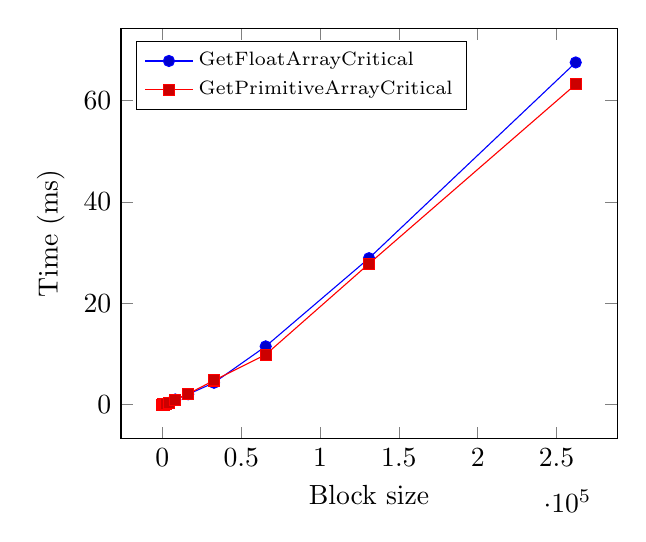
\begin{tikzpicture}
\begin{axis}[xlabel={Block size},ylabel={Time (ms)},width=0.65\linewidth,legend pos=north west,scaled y ticks = false,legend cell align=left,legend style={font=\scriptsize}]
\addplot coordinates {
(16, 0.0045)
(32, 0.0048)
(64, 0.0055)
(128, 0.0087)
(256, 0.0137)
(512, 0.0312)
(1024, 0.0667)
(2048, 0.1327)
(4096, 0.3437)
(8192, 1.0274)
(16384, 2.0687)
(32768, 4.3371)
(65536, 11.5128)
(131072, 28.9012)
(262144, 67.5020)
};
\addplot coordinates {
(16, 0.0057)
(32, 0.0050)
(64, 0.0056)
(128, 0.0089)
(256, 0.0134)
(512, 0.0348)
(1024, 0.0608)
(2048, 0.1925)
(4096, 0.3656)
(8192, 1.0051)
(16384, 2.1559)
(32768, 4.7898)
(65536, 9.8807)
(131072, 27.8158)
(262144, 63.1858)
};
\legend{GetFloatArrayCritical, GetPrimitiveArrayCritical}
\end{axis}
\end{tikzpicture}

%         &
%         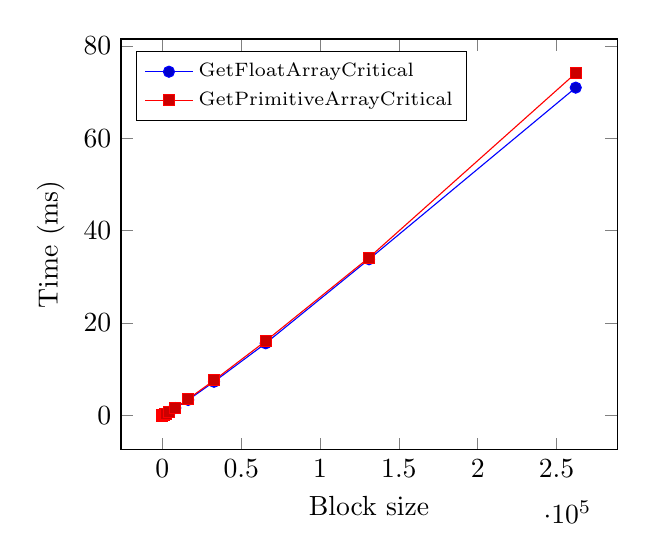
\begin{tikzpicture}
\begin{axis}[xlabel={Block size},ylabel={Time (ms)},width=0.65\linewidth,legend pos=north west,scaled y ticks = false,legend cell align=left,legend style={font=\scriptsize}]
\addplot coordinates {
(16, 0.0079)
(32, 0.0106)
(64, 0.0162)
(128, 0.0280)
(256, 0.0506)
(512, 0.1036)
(1024, 0.1917)
(2048, 0.3825)
(4096, 0.7539)
(8192, 1.6084)
(16384, 3.3681)
(32768, 7.3011)
(65536, 15.6232)
(131072, 33.8117)
(262144, 70.9477)
};
\addplot coordinates {
(16, 0.0108)
(32, 0.0150)
(64, 0.0187)
(128, 0.0286)
(256, 0.0544)
(512, 0.0961)
(1024, 0.1868)
(2048, 0.3659)
(4096, 0.8086)
(8192, 1.6133)
(16384, 3.5690)
(32768, 7.6009)
(65536, 16.1129)
(131072, 34.1650)
(262144, 74.0746)
};
\legend{GetFloatArrayCritical, GetPrimitiveArrayCritical}
\end{axis}
\end{tikzpicture}

%         \\
%         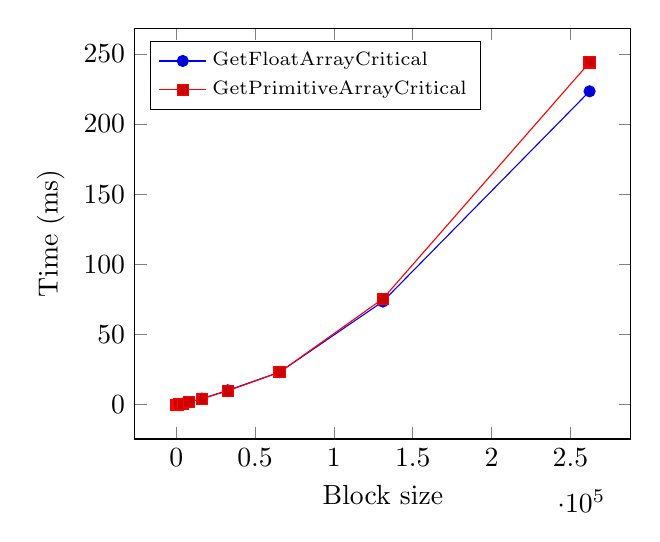
\begin{tikzpicture}
\begin{axis}[xlabel={Block size},ylabel={Time (ms)},width=0.65\linewidth,legend pos=north west,scaled y ticks = false,legend cell align=left,legend style={font=\scriptsize}]
\addplot coordinates {
(16, 0.0057)
(32, 0.0070)
(64, 0.0092)
(128, 0.0136)
(256, 0.0222)
(512, 0.0418)
(1024, 0.0970)
(2048, 0.2761)
(4096, 0.7818)
(8192, 1.8794)
(16384, 4.3304)
(32768, 10.2608)
(65536, 23.1917)
(131072, 73.5225)
(262144, 223.3088)
};
\addplot coordinates {
(16, 0.0072)
(32, 0.0086)
(64, 0.0083)
(128, 0.0115)
(256, 0.0200)
(512, 0.0366)
(1024, 0.0773)
(2048, 0.2604)
(4096, 0.7974)
(8192, 1.9326)
(16384, 4.2789)
(32768, 9.9388)
(65536, 23.1031)
(131072, 75.4942)
(262144, 243.8496)
};
\legend{GetFloatArrayCritical, GetPrimitiveArrayCritical}
\end{axis}
\end{tikzpicture}

%         &
%         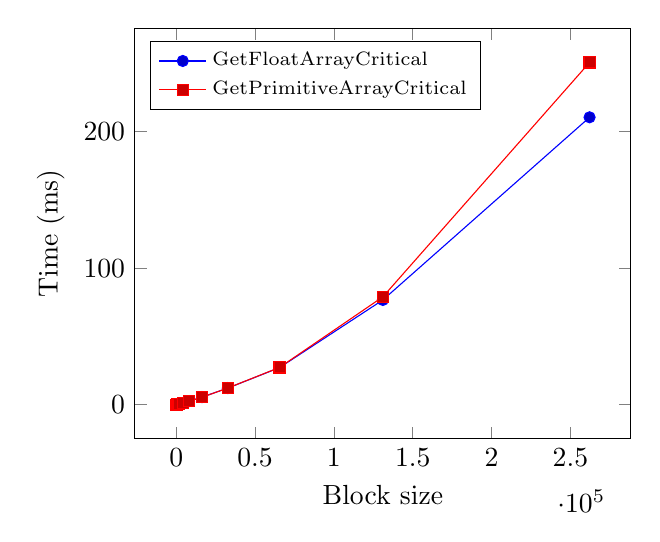
\begin{tikzpicture}
\begin{axis}[xlabel={Block size},ylabel={Time (ms)},width=0.65\linewidth,legend pos=north west,scaled y ticks = false,legend cell align=left,legend style={font=\scriptsize}]
\addplot coordinates {
(16, 0.0083)
(32, 0.0124)
(64, 0.0201)
(128, 0.0348)
(256, 0.0651)
(512, 0.1275)
(1024, 0.2659)
(2048, 0.5235)
(4096, 1.1475)
(8192, 2.6441)
(16384, 5.5785)
(32768, 12.1775)
(65536, 27.1549)
(131072, 76.6735)
(262144, 210.3414)
};
\addplot coordinates {
(16, 0.0097)
(32, 0.0132)
(64, 0.0214)
(128, 0.0342)
(256, 0.0627)
(512, 0.1225)
(1024, 0.2744)
(2048, 0.5257)
(4096, 1.1701)
(8192, 2.5845)
(16384, 5.4518)
(32768, 12.2266)
(65536, 27.2805)
(131072, 78.9501)
(262144, 250.4870)
};
\legend{GetFloatArrayCritical, GetPrimitiveArrayCritical}
\end{axis}
\end{tikzpicture}

%         \\
%         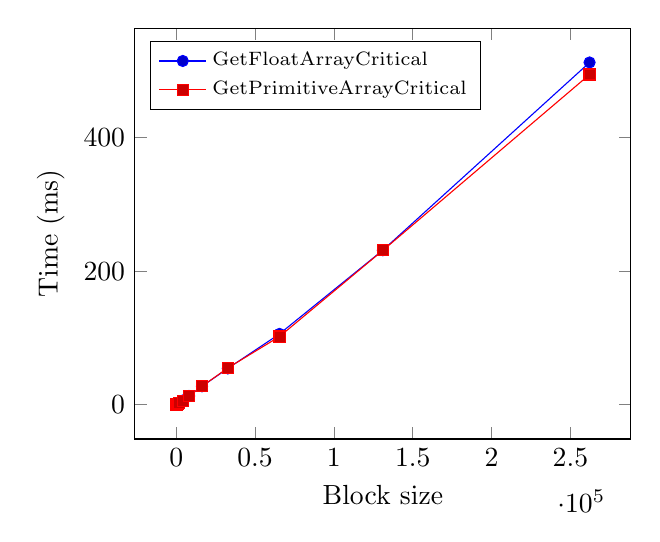
\begin{tikzpicture}
\begin{axis}[xlabel={Block size},ylabel={Time (ms)},width=0.65\linewidth,legend pos=north west,scaled y ticks = false,legend cell align=left,legend style={font=\scriptsize}]
\addplot coordinates {
(16, 0.0187)
(32, 0.0347)
(64, 0.0709)
(128, 0.1447)
(256, 0.3014)
(512, 0.6505)
(1024, 1.3689)
(2048, 2.9279)
(4096, 6.2499)
(8192, 13.1419)
(16384, 27.7314)
(32768, 54.4151)
(65536, 106.1420)
(131072, 231.5323)
(262144, 512.7674)
};
\addplot coordinates {
(16, 0.0202)
(32, 0.0368)
(64, 0.0705)
(128, 0.1434)
(256, 0.2978)
(512, 0.6379)
(1024, 1.3437)
(2048, 2.8773)
(4096, 6.1206)
(8192, 13.2345)
(16384, 27.6080)
(32768, 55.1227)
(65536, 102.1585)
(131072, 231.2663)
(262144, 494.7038)
};
\legend{GetFloatArrayCritical, GetPrimitiveArrayCritical}
\end{axis}
\end{tikzpicture}

%         &
%         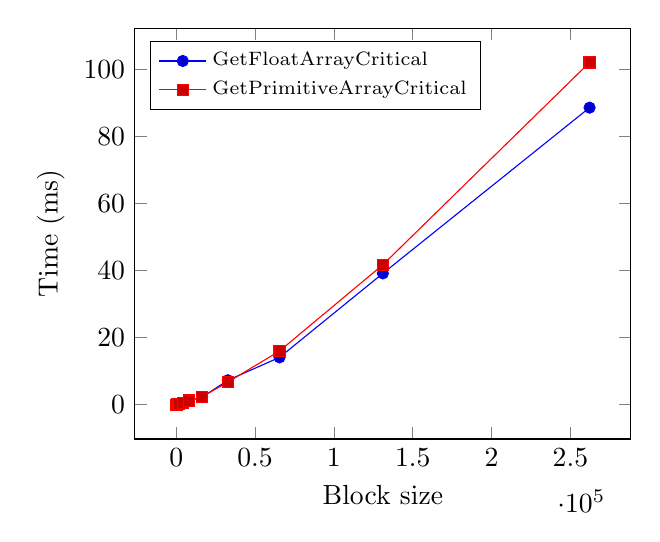
\begin{tikzpicture}
\begin{axis}[xlabel={Block size},ylabel={Time (ms)},width=0.65\linewidth,legend pos=north west,scaled y ticks = false,legend cell align=left,legend style={font=\scriptsize}]
\addplot coordinates {
(16, 0.0050)
(32, 0.0060)
(64, 0.0072)
(128, 0.0139)
(256, 0.0212)
(512, 0.0478)
(1024, 0.0885)
(2048, 0.1965)
(4096, 0.3867)
(8192, 1.1701)
(16384, 2.2685)
(32768, 7.2940)
(65536, 14.1297)
(131072, 39.1887)
(262144, 88.6356)
};
\addplot coordinates {
(16, 0.0056)
(32, 0.0069)
(64, 0.0079)
(128, 0.0131)
(256, 0.0182)
(512, 0.0461)
(1024, 0.0992)
(2048, 0.2047)
(4096, 0.4022)
(8192, 1.2470)
(16384, 2.3713)
(32768, 6.7420)
(65536, 16.0281)
(131072, 41.7620)
(262144, 102.1196)
};
\legend{GetFloatArrayCritical, GetPrimitiveArrayCritical}
\end{axis}
\end{tikzpicture}

%     \end{tabular}
%     \caption{ARR C++}
%     \label{fig:appendix:arr:line}
% \end{table}

\cleardoublepage
\fi

\end{document}
